%% NEW SMALL GUNS: https://github.com/ceebo/glider_guns
%%%%%%%%%%%%%%%%%%%%%%%%%%%%%%%%%%%%%%%%%%%%%%%%%%%%%%%%%%%%%%%%%%%%%%%%%
%%   CHAPTER: GUNS AND GLIDER STREAMS
%%%%%%%%%%%%%%%%%%%%%%%%%%%%%%%%%%%%%%%%%%%%%%%%%%%%%%%%%%%%%%%%%%%%%%%%%

\renewcommand{\chapterfolder}{glider_guns/}
\chapterimage{cover/glider_guns}
\chapter{Guns and Glider Streams}\label{chp:guns}


\vspace*{-0.4in}
\epigraph{Assembling large arrays of guns and puffers---other than getting the timing and positioning right---is about [as] difficult as assembling large objects out of Lego bricks.}{Mark D. Niemiec}
\vspace*{0.4in}


\noindent We have seen that being able to efficiently create and manipulate streams of gliders is extremely important when constructing complex objects in Life, since we can use collisions between those gliders to synthesize other objects. However, so far we have only seen how to create glider streams with a few different spacings: the period~30 stream produced by the Gosper glider gun (Section~\ref{sec:queen_bee}), the period~46 stream produced by the twin bees gun (Section~\ref{sec:twin_bees}), and the streams of period~61 and higher than we can construct via the Herschel tracks of Sections~\ref{sec:herschel_track} and~\ref{sec:conduits}. In this chapter, we look at how to construct glider guns that create gliders of any spacing and almost any positioning that we like.

%%%%%%%%%%%%%%%%%%%%%%%%%%%%%%%%%%%%%%%%%%%%%%%%%%%%%%%%%%%%%%%%%%%%%%%%%
%%   SECTION: GLIDER DELETION
%%%%%%%%%%%%%%%%%%%%%%%%%%%%%%%%%%%%%%%%%%%%%%%%%%%%%%%%%%%%%%%%%%%%%%%%%
\section{Glider Deletion}\label{sec:glider_deletion}

The first technique that we present for constructing guns of different periods is one that erases every second glider in a stream of period at least~$29$,\footnote{There is a similar reaction that can be used to double glider streams of period at least $28$---see Exercise~\ref{exer:p28_double}.} thus doubling its period (the semi-Snark\index{semi-Snark} of Section~\ref{sec:large_glider_guns} can similarly delete every second glider in a glider stream, but it only works at periods~$48$ and greater). The way this technique works is to fire two streams of the same period at each other in such a way that they synthesize a block,\footnote{In particular, this glider collision is the fifth of the block-producing collisions listed in Table~\ref{tab:2_glider_synth}.} and that block then destroys the next glider in one of the streams. A particular orientation of glider streams that works is displayed in Figure~\ref{fig:glider_delete}---one of the glider streams is erased completely (half of its gliders are destroyed in the glider-to-block collision, and the other half are destroyed by the subsequent block), while the other glider stream has half of its gliders destroyed.

\begin{figure}[!htb]
	\centering
	\embedlink{glider_delete}{\vcenteredhbox{\patternimg{0.109}{glider_delete_0}} \vcenteredhbox{\genarrow{4}} \vcenteredhbox{\patternimg{0.109}{glider_delete_4}} \vcenteredhbox{\genarrow{25}} \vcenteredhbox{\patternimg{0.109}{glider_delete_29}} \vcenteredhbox{\genarrow{29}} \vcenteredhbox{\patternimg{0.109}{glider_delete_58}}}
	\caption{If we shoot two glider streams of period at least $29$ at each other in the proper phase, one of the streams is destroyed completely while the other stream is thinned out by a factor of 2. This works because the gliders collide to form a block, and that block then destroys the next glider in the bottom stream, letting the next glider from the top stream pass by unharmed.}\label{fig:glider_delete}
\end{figure}

We can use this reaction to straightforwardly double the period of any glider gun with period~$29$ or higher, which we demonstrate in Figure~\ref{fig:guns_doubled_period} with the period~$30$ Gosper glider gun and the period~$46$ twin bees gun.\footnote{The gun in Figure~\ref{fig:guns_doubled_period}(a) is not quite the smallest known period~$60$ gun by bounding box area---see \httpsurl{catagolue.hatsya.com/object/gun_60/b3s23}. Similarly, a slightly smaller period~$92$ gun can be constructed by colliding two twin bees shuttles together directly in a clever way.}

By iterating this procedure, we can repeatedly double the period of a glider stream, thus multiplying the period of any glider stream (with period at least~$29$) by any power of two. However, what if we want to multiply the period by another number, such as $3$ or $5$? Well, we could simply try firing glider streams at each other in different ways and see if any of them do the trick---after all, we saw in Section~\ref{sec:2glidersynth} that there are only $71$ ways for two glider streams to hit each other, so it won't take too long to check them for useful combinations. And indeed, it turns out that a period-tripling configuration exists for sufficiently slow even-period glider streams,\footnote{The collision we describe here is the third one listed in the ``misc'' section of Table~\ref{tab:2_glider_synth}.} as demonstrated in Figure~\ref{fig:glider_delete2}.

% This figure can be moved 1 paragraph earlier, if desired. It is just here for spacing reasons.
\begin{figure}[!htb]
	\centering
	\begin{subfigure}{.48\textwidth}
		\centering
		\patternimglink{0.14309638554}{p60_gun}
		\caption{A period~$60$ gun that uses two Gosper glider guns.}
		\label{fig:p60_gun}
	\end{subfigure} \hfill % 
	\begin{subfigure}{.49\textwidth}
		\centering
		\patternimglink{0.111}{p92_gun}
		\caption{A period~$92$ gun that uses two twin bees guns.}
		\label{fig:p92_gun}
	\end{subfigure}
	\caption{We can use two copies of any gun with period at least $29$ to create a gun with double the period. This is demonstrated in (a) with two period~$30$ Gosper glider guns creating a period~$60$ gun, and (b) two period~$46$ twin bees guns creating a period~$92$ gun. In each case, the individual guns are outlined in \bgbox{aquaback}{aqua}, gliders that collide to create a block are outlined in \bgbox{yellowback2}{yellow}, and gliders to survive to create the new, thinner glider stream travelling to the southeast are outlined in \bgbox{greenpastel}{green}.}\label{fig:guns_doubled_period}
\end{figure}

The way that this period tripler works is largely the same as it was from the period-doubling collision from Figure~\ref{fig:glider_delete}, only slightly more complicated:\smallskip

\begin{itemize}
	\item When the first gliders in the streams collide, they leave behind a pair of blocks.\smallskip
	
	\item When the next gliders in the streams hit the blocks, they are turned into a single blinker.\smallskip
	
	\item That blinker destroys the third glider in one of the streams, and the third glider in the other stream passes by unharmed.\smallskip
\end{itemize}

% This figure can be moved 1 paragraph earlier, if desired. It is just here for spacing reasons.
\begin{figure}[!htb]
	\centering
	\embedlink{glider_delete2}{\vcenteredhbox{\patternimg{0.094}{glider_delete2_0}} \vcenteredhbox{\genarrow{6}} \vcenteredhbox{\patternimg{0.094}{glider_delete2_6}} \vcenteredhbox{\genarrow{30}} \vcenteredhbox{\patternimg{0.094}{glider_delete2_36}} \vcenteredhbox{\genarrow{66}} \vcenteredhbox{\patternimg{0.094}{glider_delete2_102}}}
	\caption{If we shoot two even-period glider streams of period at least $34$ at each other in the proper phase, one of the streams is destroyed completely while the other stream is thinned out by a factor of ~$3$.}\label{fig:glider_delete2}
\end{figure}

The effect of firing two glider streams at each other in this way is thus to completely destroy one of the streams and to destroy two-thirds of the gliders in the other. This reaction is demonstrated in Figure~\ref{fig:p138_gun}, where we use two period~$46$ twin bees guns to create a period $3 \times 46 = 138$ gun (this reaction only works for glider streams of period~$34$ or higher, so we cannot apply it to the Gosper glider gun). Also, just like before, we can use this reaction repeatedly with more and more copies of the original gun, each time multiplying the gun's period by $3$.

\begin{figure}[!htb]
	\centering
	\patternimglink{0.1}{p138_gun}
	\caption{We can use two copies of any gun with period at least~$34$ to create a gun with triple the period. Here, two period~$46$ twin bees guns are aimed at each other so as to create a period~$138$ gun.}\label{fig:p138_gun}
\end{figure}

By combining these two period-multiplying reactions together, we can multiply a gun's period by any number whose prime factorization contains only $2$ or $3$, with at least one factor of $2$. We can thus use this technique to thin out a glider stream by a factor of $4$, $6$, or $8$, for example. We can multiply a gun's period by $9$ only if the gun's period is even; otherwise a glider will strike the blinker that makes up one of the stages of the tripling reaction, at the wrong phase.\footnote{We can use the stable circuitry techniques from Section~\ref{sec:large_glider_guns} to thin out a glider stream by any factor of our choosing, but these collision-based techniques are a bit smaller and easier to use, at least for small factors.}

To fill in some of the gaps in the above list of possible multipliers, we present in Figure~\ref{fig:glider_delete_prime} some methods for thinning out a stream by a factor of $5$ or $7$.

\begin{figure}[!htb]
	\centering
	\begin{subfigure}{.48\textwidth}
		\centering
		\patternimglink{0.12}{glider_delete4}
		\caption{A collision that thins out even-period glider streams with period at least $108$ by a factor of $5$.}
		\label{fig:glider_delete4}
	\end{subfigure} \hfill % 
	\begin{subfigure}{.48\textwidth}
		\centering
		\patternimglink{0.12}{glider_delete6}
		\caption{A collision that thins out even-period glider streams with period at least $46$ by a factor of $7$.}
		\label{fig:glider_delete6}
	\end{subfigure}
	\caption{Some additional methods of multiplying the period of glider streams by small prime numbers.}\label{fig:glider_delete_prime}
\end{figure}


%%%%%%%%%%%%%%%%%%%%%%%%%%%%%%%%%%%%%%%%%%%%%%%%%%%%%%%%%%%%%%%%%%%%%%%%%
%%   SUBSECTION: FILTERS
%%%%%%%%%%%%%%%%%%%%%%%%%%%%%%%%%%%%%%%%%%%%%%%%%%%%%%%%%%%%%%%%%%%%%%%%%
\subsection{Filters}\label{sec:filters}

Another way of deleting some gliders within a stream is to use a \textbf{filter},\index{filter} which is an oscillator that pulsates or gives off a spark in such a way as to destroy some of the gliders in the stream, but not all of them (similar to how we used a Schick engine to erase some of the gliders released by a space rake in Section~\ref{sec:schick_engine}). Gliders can be destroyed by essentially any type of spark (see Figure~\ref{fig:glider_delete_spark}), so we can use many high-period sparkers to destroy gliders and thin out glider streams.

\begin{figure}[!htb]
	\centering
	\begin{subfigure}{.32\textwidth}
		\centering
		\embedlink{glider_delete_dot}{\vcenteredhbox{\patternimg{0.11}{glider_delete_dot_0}}
			\vcenteredhbox{\genarrow{5}}
			\vcenteredhbox{\patternimg{0.11}{glider_delete_dot_5}}}
		\caption{A dot spark\index{dot spark} deleting a glider.}
		\label{fig:glider_delete_dot}
	\end{subfigure} \hfill % 
	\begin{subfigure}{.32\textwidth}
		\centering
		\embedlink{glider_delete_domino}{\vcenteredhbox{\patternimg{0.11}{glider_delete_domino_0}}
			\vcenteredhbox{\genarrow{4}}
			\vcenteredhbox{\patternimg{0.11}{glider_delete_domino_4}}}
		\caption{A domino spark\index{domino spark} deleting a glider.}
		\label{fig:glider_delete_domino}
	\end{subfigure} \hfill % 
	\begin{subfigure}{.32\textwidth}
		\centering
		\embedlink{glider_delete_banana}{\vcenteredhbox{\patternimg{0.11}{glider_delete_banana_0}}
			\vcenteredhbox{\genarrow{5}}
			\vcenteredhbox{\patternimg{0.11}{glider_delete_banana_5}}}
		\caption{A banana spark\index{banana spark} deleting a glider.}
		\label{fig:glider_delete_banana}
	\end{subfigure}
	\caption{Many different sparks can be used to delete gliders.}\label{fig:glider_delete_spark}
\end{figure}

For example, if we place a period~$8$ blocker\index{blocker} next to a glider stream of period $8n+4$ $(n \geq 2$), it destroys every second glider in the stream, thus doubling its period. Similarly, the period~$16$ oscillator ``Rich's p16'' from Figure~\ref{fig:rich_p16} emits a banana spark that can be used to double the period of any glider stream with period $16n+8$ ($n \geq 1$),\footnote{Rob's p16 works just as well for this purpose---see Exercise~\ref{exer:robs_p16_smaller_p16_gun}.} and the period~$22$ oscillator from Figure~\ref{fig:period_22} emits a domino spark that can be used to double the period of any glider stream with period $22n+11$ ($n \geq 1$). These period-doubling filters are illustrated for streams of period~$20$, $24$, and~$33$ in Figure~\ref{fig:glider_filters}.\index{Rich's p16}\index{Rob's p16}\index{blocker}\index{Jason's p22}

\begin{figure}[!htb]
	\centering
	\begin{subfigure}{.31\textwidth}
		\centering
		\patternimglink{0.13014522821}{blocker_glider_filter}
		\caption{The dot spark from a blocker can be used to destroy every other glider in a stream of period~$20$ (or $8n+4$ for any $n \geq 2$).}
		\label{fig:blocker_glider_filter}
	\end{subfigure} \hfill % 
	\begin{subfigure}{.31\textwidth}
		\centering
		\patternimglink{0.0953343465}{richs_p16_glider_filter}
		\caption{The banana spark from Rich's p16 can be used to destroy every other glider in a stream of period~$24$ (or $16n+8$ for any $n \geq 1$).}
		\label{fig:richs_p16_glider_filter}
	\end{subfigure} \hfill % 
	\begin{subfigure}{.31\textwidth}
		\centering
		\patternimglink{0.085}{p22_glider_filter}
		\caption{A domino spark from Jason's p22 can be used to destroy every other glider in a stream of period~$33$ (or $22n+11$ for any $n \geq 1$).}
		\label{fig:p22_glider_filter}
	\end{subfigure}
	\caption{Some filters (highlighted in \bgbox{aquaback}{aqua}) that can be used to double the period of certain glider streams.}\label{fig:glider_filters}
\end{figure}

For a filter oscillator to work correctly, it's generally necessary that the period of the oscillator shares some factor (greater than one) with the period of the glider stream being thinned. Otherwise, all possible combinations of oscillator spark and glider position will eventually appear in the evolution of the pattern, and some of those combinations will usually cause a chaotic explosion instead of a clean glider deletion.

% Mention other filters. p6 pipsquirter? Some others? Or exercise at least?
% Exercise: use two filters to turn p20 into p80 (solution: blocker followed by Rich/Rob p16)


%%%%%%%%%%%%%%%%%%%%%%%%%%%%%%%%%%%%%%%%%%%%%%%%%%%%%%%%%%%%%%%%%%%%%%%%%
%%   SUBSECTION: GLIDER INSERTION
%%%%%%%%%%%%%%%%%%%%%%%%%%%%%%%%%%%%%%%%%%%%%%%%%%%%%%%%%%%%%%%%%%%%%%%%%
\section{Glider Insertion}\label{sec:glider_insertion}

Our next technique is one that is complementary to that of the previous section: it lets us thicken glider streams (i.e., it lets us decrease their period) rather than thin them. The main idea behind this trick is to collide two or more spaceships in such a way as to produce a single glider that fits in a stream's gap. Unfortunately, this technique in its simplest form is very rarely useful, since there are only two 2-glider collisions that result in a single glider (refer back to Table~\ref{tab:2_glider_synth}), one of which results in a glider going in the \emph{same} direction as one of the input gliders, and the other of which results in a glider going in the \emph{opposite} direction of one of the input gliders. In particular, neither of these glider-producing $2$-glider collisions results in a glider travelling \emph{perpendicular} to both input gliders, which is what we really want.

Fortunately, there are a few other ways of colliding spaceships together to get around this problem. The first such method is to use one more glider: the $3$-glider collisions called \textbf{tees}\index{tee} that we introduced back in Table~\ref{tab:3_glider_synth} produces an output glider that is perpendicular to all $3$ input gliders (see Figure~\ref{fig:tee}). Another solution to this problem is to instead collide a glider with a lightweight spaceship as in Figure~\ref{fig:lwss_reflect_glider}, which has the advantage that an LWSS never travels in the same direction as a glider, so we typically have a wider selection of possible orientations to make the collision happen without interfering with other gliders in the stream.

\begin{figure}[!htb]
	\centering
	\begin{subfigure}{.48\textwidth}
		\centering
		\embedlink{tee}{\vcenteredhbox{\patternimg{0.11}{tee_0}} \vcenteredhbox{\genarrow{16}} \vcenteredhbox{\patternimg{0.11}{tee_16}}}
		\caption{A \textbf{tee}: a collision of $3$ gliders that results in a single glider perpendicular to the input gliders.}
		\label{fig:tee}
	\end{subfigure} \ \ \ \ % 
	\begin{subfigure}{.48\textwidth}
		\centering
		\embedlink{lwss_reflect_glider}{\vcenteredhbox{\patternimg{0.11}{lwss_reflect_glider_0}} \vcenteredhbox{\genarrow{12}} \vcenteredhbox{\patternimg{0.11}{lwss_reflect_glider_12}}}
		\caption{A collision between a lightweight spaceship and a glider that rotates the glider by $90$ degrees.}
		\label{fig:lwss_reflect_glider}
	\end{subfigure}
	\caption{Two methods of changing the direction of a glider so that it can be inserted into another glider stream. These techniques help us create glider guns with a wide variety of periods, and are also extremely useful for creating guns that make use of syntheses with tightly spaced gliders.}\label{fig:glider_insert_methods}
\end{figure}

These collisions can be used to insert additional gliders into an already-existing glider stream, thus decreasing its period. For example, the glider gun displayed in Figure~\ref{fig:p23_gun} uses the LWSS--glider collision to insert additional gliders into a period~$46$ glider stream coming from a twin bees gun, thus converting it into a period~$23$ gun (compare with the period~$23$ gun that we saw back in Figure~\ref{fig:twin_bees_p23_gun}).

\begin{figure}[!htb]
	\centering
	\patternimglink{0.123}{p23_gun}
	\caption{A period~$23$ glider gun constructed from several period~$46$ glider guns. The top-left glider gun in \bgbox{magentaback}{magenta} fires a period~$46$ stream of gliders. To interlace this stream with another period~$46$ stream of gliders (outlined in \bgbox{greenpastel}{green}), we use the LWSS--glider collision of Figure~\ref{fig:lwss_reflect_glider}: the glider in that collision is created by the glider gun outlined in \bgbox{yellowback2}{yellow}, while the LWSS is created by the LWSS gun (which we introduced in Figure~\ref{fig:twin_bees_p46_lwss_gun}) outlined in \bgbox{aquaback}{aqua}.}\label{fig:p23_gun}
\end{figure}

Unfortunately, the tee from Figure~\ref{fig:tee} cannot be used to produce glider streams with period smaller than~$25$, and the LWSS--glider collision from Figure~\ref{fig:lwss_reflect_glider} is similarly limited to periods of at least $22$; the temporary debris created by these collisions interferes with the rest of the glider stream at lower periods. So for example, these reactions cannot be used to transform multiple Gosper glider guns into a period~$15$ gun, despite the fact that period~$15$ glider streams are indeed possible.

One way of constructing guns for even tighter glider streams (all the way down to period~$14$, which is the smallest possible) is to instead use the reaction from Figure~\ref{fig:lwss_squish}(a), in which two sparks transform a lightweight spaceship into a glider with essentially no debris occurring outside of that transformation.\footnote{This reaction was found by Dietrich Leithner no later than 1994.} The first of these sparks (which can be of essentially any type, but is typically a dot, a finger, or a domino coming from a pipsquirter)\index{pipsquirter} starts destroying the lightweight spaceship and can be provided by a wide variety of oscillators. The second spark (which must be a domino or duoplet) then transforms the dying LWSS into the desired glider. However, that second spark is a bit tricker to get into place, as it must be provided directly adjacent to the glider stream, so it is typically provided by another dying object like an LWSS or a Herschel. Some methods of providing these two sparks are illustrated in Figure~\ref{fig:lwss_squish}(b--f).

\begin{figure}[!htb]
	\centering
	\begin{tabular}{@{}ccc@{}}
		\begin{subfigure}{0.49\textwidth}
			\centering\vspace*{1cm}
			\embedlink{lwss_squish}{\vcenteredhbox{\patternimg{0.11}{lwss_squish_0}} \vcenteredhbox{\genarrow{5}} \vcenteredhbox{\patternimg{0.11}{lwss_squish_5}} \vcenteredhbox{\genarrow{1}} \vcenteredhbox{\patternimg{0.11}{lwss_squish_6}}}
			\caption{A clean glider insertion using an LWSS and two sparks.}
			\label{fig:lwss_squish_sparks}
		\end{subfigure} & \begin{subfigure}{.245\textwidth}
			\centering
			\patternimg{0.10604}{lwss_squish_pip}
			\caption{p$6$ insertion via unix and pipsquirter.}
			\label{fig:lwss_squish_pip}
		\end{subfigure} & \begin{subfigure}{.205\textwidth}
			\centering
			\patternimg{0.08419484978}{lwss_squish_blinker}
			\caption{Insertion that works at any period.}
			\label{fig:lwss_squish_blinker}
		\end{subfigure} \\[2cm] \begin{subfigure}{0.49\textwidth}
			\centering
			\patternimg{0.099}{lwss_squish_herschel}
			\caption{Insertion via a pipquirter and a Herschel.}
			\label{fig:lwss_squish_herschel}
		\end{subfigure} & \begin{subfigure}{.245\textwidth}
			\centering
			\patternimg{0.099}{lwss_squish_p4}
			\caption{p$4$ insertion.}
			\label{fig:lwss_squish_p4}
		\end{subfigure} & \begin{subfigure}{.205\textwidth}
			\centering
			\patternimg{0.099}{lwss_squish_p5}
			\caption{p$15$ insertion.}
			\label{fig:lwss_squish_p5}
		\end{subfigure}
	\end{tabular}
	\caption{(a) A dot spark (in \bgbox{orangeback}{orange}), followed by a domino spark~$5$ generations later (in \bgbox{greenback}{green}) can be used to transform a lightweight spaceship into a glider so cleanly that it can be used to fill in gaps in p$14$ glider streams---the tightest streams possible. The first spark can be provided by (b,d,e,f) a wide variety of different oscillators or (c) a two-glider collision. The second spark can be provided either via (b,e,f) an LWSS being destroyed by an oscillator, (c) a blinker + glider + LWSS collision, or (d) a Herschel conduit.}\label{fig:lwss_squish}\vspace*{0.2cm}
\end{figure}

To illustrate the utility of this reaction, we can now construct a period~$15$ glider gun by making use of several copies of the p$30$ Gosper glider gun, much like we constructed a period~$23$ glider gun out of many copies of the p$46$ twin bees gun in Figure~\ref{fig:p23_gun}. In particular, since the reaction of Figure~\ref{fig:lwss_squish_p5} works so naturally at period~$15$, we make use of it via $7$ Gosper glider guns: $1$ to create the initial p$30$ glider stream, and $3$ for each of the two lightweight spaceships that we smash together between a pentadecathlon and middleweight volcano. The completed p$15$ gun is displayed in Figure~\ref{fig:p15_gun}.\index{pentadecathlon}\index{middleweight!volcano}

\begin{figure}[!htb]
	\centering
	\patternimglink{0.1185}{p15_gun}
	\caption{A period~$15$ glider gun constructed from several period~$30$ Gosper glider guns. The top-left glider gun in \bgbox{magentaback}{magenta} fires a period~$30$ stream of gliders. To interlace this stream with another period~$30$ stream of gliders (outlined in \bgbox{greenpastel}{green}), we use the LWSS--LWSS--pentadecathlon--middleweight volcano collision of Figure~\ref{fig:lwss_squish_p5}.}\label{fig:p15_gun}
\end{figure}

% EXERCISE: introduce alternate p15 version that leads to smaller p15 gun


%%%%%%%%%%%%%%%%%%%%%%%%%%%%%%%%%%%%%%%%%%%%%%%%%%%%%%%%%%%%%%%%%%%%%%%%%
%%   SUBSECTION: STREAMS OF OTHER SPACESHIPS
%%%%%%%%%%%%%%%%%%%%%%%%%%%%%%%%%%%%%%%%%%%%%%%%%%%%%%%%%%%%%%%%%%%%%%%%%
\section{Streams of Other Spaceships}

Since most ways of implementing the glider insertion reaction of Figure~\ref{fig:lwss_squish} rely so heavily on the use of lightweight spaceships, we now briefly discuss how to efficiently create and manipulate lightweight (as well as middleweight and heavyweight) spaceships. We of course can create streams of any of these xWSSes simply via the various $3$-glider syntheses that we saw in Chapter~\ref{chp:glider_synthesis}, but we are going to focus on reactions that let us save space over this na\"ive method.

One particularly cheap way of creating lightweight and middleweight spaceships is the conduit displayed in Figure~\ref{fig:H_plus_G_to_WSS}, which converts a glider and a Herschel into whichever of the other two spaceships is desired (the only difference in these two reactions is the relative timing between the input Herschel and glider). Since the Herschel that is used in that collision creates a glider anyway, and that glider can simply be reflected back so as to collide with the next Herschel, this conduit can turn a Herschel stream into an LWSS stream or an MWSS stream reasonably directly.\footnote{This reaction only works with \emph{streams} of Herschels, rather than individual Herschels, since each Herschel must collide with the first natural glider of a Herschel that came before it. The period of that stream can be modified straightforwardly by adjusting the reflectors---see Exercise~\ref{exer:p156_adjust_lwss}.} However, the tight spacing of the required reflectors is such that this technique works best for streams whose period is a multiple of $3$ or $4$, since p$3$, p$4$, and p$6$ bumpers are some of the only reflectors that fit so close together.

\begin{figure}[!htb]
	\centering
	\begin{subfigure}{0.48\textwidth}
		\centering
		\patternimglink{0.08616147308}{p14_pieces_lwss}
		\caption{A period~$156$ Herschel stream being converted into an LWSS stream.}\label{fig:p14_pieces_lwss}
	\end{subfigure} \hfill \begin{subfigure}{0.49\textwidth}
		\centering
		\patternimglink{0.079}{H_G_to_MWSS}
		\caption{A period~$171$ Herschel stream being converted into an MWSS stream.}\label{fig:H_G_to_MWSS}
	\end{subfigure}
	\caption{A conduit (highlighted in \bgbox{greenpastel}{green}) that can convert a Herschel and glider collision into either (a) an LWSS or (b) an MWSS. By reflecting the first natural glider of the input Herschel (via the bumpers highlighted in \bgbox{yellowback2}{yellow}), this conduit can convert a Herschel stream into either an LWSS stream or an MWSS stream.}\label{fig:H_plus_G_to_WSS}
\end{figure}

To create a reasonably small lightweight or middleweight spaceship gun of a large period, we can now simply attach this mechanism to the output of any sufficiently high-period glider gun of our choosing, with a syringe in between (as well as other Herschel conduits, as needed, for spacing reasons). For example, the gun in Figure~\ref{fig:p84_lwss_gun_adjustable} uses this technique to fire a period~$84$ stream of lightweight spaceships.

However, since this mechanism uses a stream of Herschels as input, we can often construct even smaller LWSS guns by feeding Herschel into it directly from a Herschel track, rather than feeding them in via a glider gun and a syringe. A slightly smaller period~$84$ LWSS gun that uses this technique is displayed in Figure~\ref{fig:p84_lwss_gun}.

\begin{figure}[!htb]
	\centering
	\begin{subfigure}{0.45\textwidth}
		\centering
		\patternimglink{0.086}{p84_lwss_gun_adjustable}
		\caption{A p$84$ version of the adjustable glider gun from Figure~\ref{fig:p80_adjustable_gun} (highlighted in \bgbox{orangeback2}{orange}) whose output is converted into lightweight spaceships.}\label{fig:p84_lwss_gun_adjustable}
	\end{subfigure} \hfill \begin{subfigure}{0.52\textwidth}
		\centering
		\patternimglink{0.125}{p84_lwss_gun}
		\caption{A p$84$ Herschel loop whose output is converted into LWSSes. The loop is sustained by the first natural glider of a Herschel being reflected (by the reflectors highlighted in \bgbox{yellowback2}{yellow}) back into a syringe.}\label{fig:p84_lwss_gun}
	\end{subfigure}
	\caption{Two p$84$ lightweight spaceship guns that make use of the Herschel-to-LWSS mechanism of Figure~\ref{fig:H_plus_G_to_WSS}(a) (highlighted in \bgbox{greenpastel}{green}). Syringes are highlighted in \bgbox{aquaback}{aqua} and Fx77 Herschel conduits (highlighted in \bgbox{magentaback}{magenta}) are used for spacing reasons.}\label{fig:p84_lwss_gun_both}
\end{figure}

We can also delete lightweight spaceships from a stream in much the same ways that we do with gliders. For example, a spark of pretty much any type can destroy a lightweight spaceship, so we can use sparky oscillators to filter (i.e., thin out) LWSS streams. Figure~\ref{fig:lwss_filters} illustrates to examples of how this technique can be used to double, or even triple, streams of certain periods. Another method of doubling the period of an LWSS stream, which has the advantage of working at any sufficiently large period, was presented in Exercise~\ref{exer:twin_primer}.

Similarly, if we want to \emph{decrease} the period of an xWSS stream, we can perform insertion just like we did with gliders. One possible method of inserting an LWSS into a stream is to make use of one of the three-glider syntheses from Table~\ref{tab:3_glider_synth}. However, even the fastest and cleanest of these syntheses can only decrease the period of an LWSS stream down to $22$. Since the minimum possible periods of LWSS, MWSS, and HWSS streams are 14, 16, and 18, respectively, we would like a cleaner reaction that can produce these even tighter streams. The tightest known reaction of this type is displayed in Figure~\ref{fig:lwss_insertion_p18}. It uses a whopping $10$ gliders to carefully place a lightweight spaceship between two others that are $36$ generations apart, resulting in a p$18$ LWSS stream.

Fortunately, we do not actually need to come up with new insertion mechanisms for streams of middleweight or heavyweight spaceships, since there are numerous ways of colliding spaceships with the back end of an LWSS so as to ``upgrade'' it to an MWSS, and there are similarly numerous ways of ``upgrading'' an MWSS to an HWSS. Some methods that work even with tightly packed period~18 xWSS streams are displayed in Figure~\ref{fig:xwss_upgrade}.\footnote{Much simpler methods are known for higher-period streams. See Exercise~\ref{exer:lwss_to_hwss_upgrade}, for example.}

% ideally 2 paragraphs earlier
\begin{figure}[!htb]
	\centering
	\begin{subfigure}{0.28\textwidth}
		\centering
		\patternimglink{0.09}{lwss_filter_tnosed_p4}
		\caption{The finger spark from a T-nosed p4\index{T-nosed p4} can be used to destroy every other LWSS in a stream of period $4n+2$ for any $n \geq 3$.}\label{fig:lwss_filter_tnosed_p4}
	\end{subfigure} \hfill \begin{subfigure}{0.35\textwidth}
		\centering\vspace*{0cm}
		\patternimglink{0.1}{lwss_filter_blocker}
		\caption{The dot spark from a blocker\index{blocker} can be used to destroy every other LWSS in a stream of period $8n+4$ for any $n \geq 2$.}\label{fig:lwss_filter_blocker}
	\end{subfigure} \hfill \begin{subfigure}{0.335\textwidth}
		\centering
		\patternimglink{0.07880829015}{lwss_filter_pentadecathlon}
		\caption{The thumb and domino sparks from a pentadecathlon\index{pentadecathlon} can be used to destroy two out of every three LWSSes in a stream of period $15n+5$ or $15n+10$ for any $n \geq 1$.}\label{fig:lwss_filter_pentadecathlon}
	\end{subfigure}
	\caption{Some filters (highlighted in \bgbox{aquaback}{aqua}) that can be used to double or triple the period of certain LWSS streams.}\label{fig:lwss_filters}
\end{figure}

% ideally 1 paragraph earlier
\begin{figure}[!htb]
	\centering
	\embedlink{lwss_insertion_p18}{\vcenteredhbox{\patternimg{0.125}{lwss_insertion_p18_0}} \vcenteredhbox{\genarrow{84}} \vcenteredhbox{\patternimg{0.125}{lwss_insertion_p18_84}}}
	\caption{A 10-glider collision that can be used to insert an LWSS into streams with period as low as 36, resulting in LWSS streams with period as low as 18. The cells displayed in \bgbox{redback}{red} die off in another 72 generations. Found by Chris Cain in October 2018.}\label{fig:lwss_insertion_p18}
\end{figure}

Just like glider insertion can be used to create glider guns with small periods, LWSS insertion can be used to create xWSS guns with small periods. We leave the explicit construction of such guns to Exercise~\ref{exer:pseudo_xwss_gun_p18} though, as we have carried out this type of task several times already at this point (and we will do it again for glider guns in the next section). However, these techniques can only be used to create xWSS guns with period at least 18. Even though LWSS and MWSS streams can be packed to have periods as small as~14 and~16, respectively, no guns of those periods for those spaceships are currently known, since there is no known xWSS insertion reaction that is clean and tight enough.


%%%%%%%%%%%%%%%%%%%%%%%%%%%%%%%%%%%%%%%%%%%%%%%%%%%%%%%%%%%%%%%%%%%%%%%%%
%%   SUBSECTION: GLIDER GUNS OF ANY PERIOD
%%%%%%%%%%%%%%%%%%%%%%%%%%%%%%%%%%%%%%%%%%%%%%%%%%%%%%%%%%%%%%%%%%%%%%%%%
\section{Glider Guns of Any Period}\label{sec:glider_gun_any_period}

We have already seen a few methods of constructing glider guns of any suitably large period of our choosing---we can use Herschel tracks as described in Sections~\ref{sec:herschel_track} and~\ref{sec:conduits} to create guns of any period~$62$ or greater, the adjustable-period glider gun of Figure~\ref{fig:p80_adjustable_gun} to create guns of any period~$80$ or greater, and the period multipliers of Section~\ref{sec:large_glider_guns} to create guns with extraordinarily large periods. However, none of those methods can create a glider gun with very \emph{small} period, like~$14$.

% ideally 2 paragraphs earlier
\begin{figure}[!htb]
	\centering
	\begin{subfigure}{0.525\textwidth}
		\centering
		\embedlink{lwss_upgrade}{\vcenteredhbox{\patternimg{0.12}{lwss_upgrade_0}} \vcenteredhbox{\genarrow{12}} \vcenteredhbox{\patternimg{0.12}{lwss_upgrade_12}}}
		\caption{Two lightweight spaceships can be used to convert an LWSS into an MWSS.}\label{fig:lwss_upgrade}
	\end{subfigure} \hfill \begin{subfigure}{0.445\textwidth}
		\centering
		\embedlink{lwss_upgrade}{\vcenteredhbox{\patternimg{0.0882644628}{mwss_upgrade_0}} \vcenteredhbox{\genarrow{12}} \vcenteredhbox{\patternimg{0.0882644628}{mwss_upgrade_12}}}
		\caption{Six gliders can be used to convert an MWSS into an HWSS.}\label{fig:mwss_upgrade}
	\end{subfigure}
	\caption{Some ways of firing lightweight spaceships or gliders at LWSS and MWSS streams so as to ``upgrade'' them to MWSS and HWSS streams. These reactions are clean enough to work at the minimum possible periods (16 for the LWSS $\rightarrow$ MWSS conversion and 18 for the MWSS $\rightarrow$ HWSS conversion).}\label{fig:xwss_upgrade}
\end{figure}

By making use of the glider insertion reaction of Figure~\ref{fig:lwss_squish}, we can now fill in this gap in our knowledge and construct glider guns of all periods~$14$ and greater---we just create a gun whose period is a suitably large multiple of the period that we actually want, and then repeatedly use multiple copies of this gun and the glider insertion reaction to fill in the gaps in its glider stream. For example, to create a period~$14$ gun, we could use Herschel tracks to construct a gun of period~$14 \times 5 = 70$ to create a p$70$ glider stream, and then use multiple copies of that gun to do glider insertion $4$ times between each pair of gliders in that stream.\footnote{The first period~14 glider gun was built by Dietrich Leithner in November 1994 using these same ideas (and the same glider insertion reaction).} However, the resulting p$14$ gun would be quite large---recall that creating a p$15$ gun required \emph{seven} p$30$ guns in Figure~\ref{fig:p15_gun}, and that was just to perform a single glider insertion.

In order to construct a somewhat smaller p$14$ glider gun using these same ideas, we instead use a period~$14 \times 6 = 84$ stream as our starting point, so that we can make use of the syringe in our circuitry (recall that its repeat time is $78$~generations). It is straightforward to construct a period~$84$ glider gun using the adjustable-period gun of Figure~\ref{fig:p80_adjustable_gun}, for example,\footnote{In fact, we already did this in Figure~\ref{fig:p84_lwss_gun_both}.} but if we are slightly more clever then we can actually build a gun that places \emph{two} of the six gliders that we need to bring a p$84$ stream down to p$14$. In particular, if we use the NE30T3\index{NE30T3} H-to-2G edge-shooting conduit from Figure~\ref{fig:herschel_to_glider_edge_4}, we can reflect one of its output gliders so as to be on the same lane as the other one. Figure~\ref{fig:p14_pieces_p84} illustrates how to use this technique to construct a p$84$ gun that emits $2$ out of every $3$ gliders in a p$28$ stream (or equivalently, $2$ out of every $6$ gliders in a p$14$ stream).\footnote{By rearranging the reflectors in this gun slightly, its period can be adjusted relatively straightforwardly---see Exercise~\ref{exer:p28_adjust_29}.}

\begin{figure}[!htb]
	\centering
	\patternimglink{0.1}{p14_pieces_p84}
	\caption{A p$84$ gun that emits $2$ out of $3$ gliders in a p$28$ stream. The central Herschel is fed through NE30T3 (highlighted in \bgbox{greenpastel}{green}) so as to create two output gliders, one of which is reflected (via standard reflectors like bumpers, bouncers, and Snarks, highlighted in \bgbox{yellowback2}{yellow}) into the same lane as the other one. The first natural glider of the central Herschel is similarly reflected and then injected into a syringe (highlighted in \bgbox{aquaback}{aqua}) so as to recreate itself (just as in the gun from Figure~\ref{fig:p84_lwss_gun}).}
	\label{fig:p14_pieces_p84}
\end{figure}

By making use of these reactions, we can create the period~$14$ glider gun displayed in Figure~\ref{fig:p14_gun}. This particular gun is not optimized at all---by squeezing its components together more carefully, it could be made roughly 50\% smaller (when measuring size according to bounding box area). The smallest known p$14$ gun\footnote{See \httpsurl{catagolue.hatsya.com/object/gun_14/b3s23}.} is roughly half as tall, wide, and populous as ours, but uses basically the same mechanisms that we used here---they are just packed together somewhat more cleverly and rely on three period~$42$ guns instead of five period~$84$ guns.

\begin{figure}[!htbp]
	\centering
	\patternimglink{0.1025}{p14_gun}
	\caption{A period~$14$ glider gun that uses the p$84$ two-glider gun from Figure~\ref{fig:p14_pieces_p84} (highlighted in \bgbox{magentaback}{magenta}), as well as four copies of a p$84$ glider insertion mechanism (highlighted in \bgbox{aquaback}{aqua}, \bgbox{greenpastel}{green}, \bgbox{yellowback2}{yellow}, and \bgbox{orangeback2}{orange}) to reduce the period of the stream down to~$84/6 = 14$. The glider insertion mechanisms works via the reaction from Figure~\ref{fig:lwss_squish_herschel}, which is fed by the p$84$ LWSS gun of Figure~\ref{fig:p84_lwss_gun} and a Herschel that is generated by another copy of the same p$84$ Herschel loop.}\label{fig:p14_gun}
\end{figure}



%%%%%%%%%%%%%%%%%%%%%%%%%%%%%%%%%%%%%%%%%%%%%%%%%%%%%%%%%%%%%%%%%%%%%%%%%
%%   SUBSECTION: TRUE PERIOD GUNS
%%%%%%%%%%%%%%%%%%%%%%%%%%%%%%%%%%%%%%%%%%%%%%%%%%%%%%%%%%%%%%%%%%%%%%%%%
\section{True-Period Guns}\label{sec:true_period_guns}

While we now know how to construct glider guns of every period greater than or equal to $14$, many of them are somewhat artificial---they oscillate at a higher period than (and necessarily a multiple of) the stream that they produce. For example, the gun of Figure~\ref{fig:p15_gun} actually oscillates at period~$30$, despite producing a glider stream of period~$15$, and the gun of Figure~\ref{fig:p14_gun} oscillates at period~$84$, despite producing a glider stream of period~$14$. Such guns are called \textbf{pseudo-period guns}\index{pseudo-period gun}, and the new low-period guns that we introduced in this chapter are all of this type.

There is nothing inherently wrong with pseudo-period guns, but it seems natural to ask whether or not we can construct guns of arbitrary periods that actually oscillate at the same period as their stream (i.e., guns that do not make use of techniques like glider insertion to decrease the period of the stream that they produce). We call such guns \textbf{true-period guns}\index{true-period gun}, and examples include all of the guns that we saw prior to this chapter, such as the p$30$ Gosper glider gun\index{Gosper glider gun} and the p$46$ twin bees gun\index{twin bees!gun}.

In general, using glider insertion to decrease the period of a gun's stream results in a pseudo-period gun, but using filters or the glider deletion methods of Section~\ref{sec:glider_deletion} to \emph{increase} the period of its glider stream results in a true-period gun (e.g., the p$60$ gun from Figure~\ref{fig:p60_gun} that uses two Gosper glider guns is a true-period gun). Constructing true-period guns with small period\footnote{Herschel tracks can be used to create true-period guns of large period (period~$62$ and larger, in particular).} is much more difficult than the same task for pseudo-period guns, since we cannot just manipulate gliders themselves to get the period we desire, but rather must actually develop new glider-generating mechanisms.

There are just a few methods that are known for creating true-period glider guns, and it is typically difficult to get them to work for small periods. A brief summary of the known true-period guns of these few small periods is presented in Table~\ref{tab:true_period_glider_gun}, and the next few subsections illustrate and describe their construction.\footnote{Unfortunately, it probably will not be long before this list of true-period guns becomes out of date ($7$ new periods were discovered while this book was being written!), so a perhaps more up-to-date list of known true-period gun periods can be found at \httpsurl{conwaylife.com/wiki/Gun} and \httpsurl{conwaylife.com/wiki/LifeWiki:Game_of_Life_Status_page\#Glider_gun_true-periods}.}

\begin{table}[!htbp]\vspace*{0.02in}
	\begin{center}		
		\begin{tabular}{ccll}
			\toprule
			Period & Year & Original Discoverer & Example and Notes \\ \midrule
			20 & 2013 & \specialcelll[t]{Matthias Merzenich \\ Noam Elkies} & \specialcelll[t]{{\small$\bullet$} upcoming Figure~\ref{fig:p20_glider_gun} \\ {\small$\bullet$} smaller ones now known} \\
			\rowcolor{gray!20} 21, 42 & 2021 & \specialcelll[t]{Tanner Jacobi \\ David Raucci} & Exercise~\ref{exer:p21_glider_gun} \\
			22 & 2000 & \specialcelll[t]{David Eppstein \\ Jason Summers} & upcoming Figure~\ref{fig:p22_glider_gun} \\
			\rowcolor{gray!20} 24, 48 & 1997 & Noam Elkies & upcoming Figure~\ref{fig:p24_glider_gun} \\
			28 & 2020 & \specialcelll[t]{Matthias Merzenich \\ Paul Callahan} & upcoming Figure~\ref{fig:p28_glider_gun} \\
			\rowcolor{gray!20} 30 & 1970 & Bill Gosper & Gosper glider gun (Figure~\ref{fig:gosper_glider_gun}) \\
			32 & 2021 & \specialcelll[t]{Matthias Merzenich \\ David Raucci} & \specialcelll[t]{{\small$\bullet$} smallest known is in the upcoming Figure~\ref{fig:p32_glider_gun} \\ {\small$\bullet$} first known was found just a few days earlier} \\
			\rowcolor{gray!20} 33 & 2018 & \specialcelll[t]{Arie Paap \\ Matthias Merzenich} & upcoming Figure~\ref{fig:p33_gun} \\
			36 & 2004 & Jason Summers & upcoming Figure~\ref{fig:p36_gun} \\
			\rowcolor{gray!20} 40 & 2013 & \specialcelll[t]{Adam P. Goucher \\ Matthias Merzenich \\ Jason Summers} & \specialcelll[t]{{\small$\bullet$} smallest known (Figure~\ref{fig:p20_glider_gun}) uses a blocker to \\ \hphantom{\small$\bullet$} filter the p$20$ gun \\ {\small$\bullet$} first known (not displayed) was found $3$~months earlier} \\
			44 & 1992 & David Buckingham & improved a bit in 1997 by Paul Callahan (Figure~\ref{fig:p44_glider_gun}) \\
			\rowcolor{gray!20} 45 & 2010 & Matthias Merzenich & upcoming Figure~\ref{fig:p45_gun} \\
			46 & 1971 &	Bill Gosper & twin bees gun (Figure~\ref{fig:twin_bees_gun}) \\
			\rowcolor{gray!20} 49 & 2021 & \specialcelll[t]{Tanner Jacobi \\ ``hotcrystal0'' \\ ``wwei23''} & \specialcelll[t]{{\small$\bullet$} see Exercise~\ref{exer:p51_49_guns}\\ {\small$\bullet$} the p51 gun uses the same base reaction} \\
			50 & 1996 & \specialcelll[t]{Dean Hickerson \\ Noam Elkies} & \specialcelll[t]{{\small$\bullet$} Figure~\ref{fig:p50_true_gun} shows roughly the smallest known \\ {\small$\bullet$} first known (not displayed) used Exercise~\ref{exer:traffic_jam}} \\
			\rowcolor{gray!20} 51 & 2021 & \specialcelll[t]{Luka Okanishi} & \specialcelll[t]{see Exercise~\ref{exer:p51_49_guns}} \\
			52 & 2018 & \specialcelll[t]{Dave Greene \\ Chris Cain \\ Adam P. Goucher \\ Matthias Merzenich} & \specialcelll[t]{{\small$\bullet$} smallest known (Figure~\ref{fig:p52_gun}) was constructed in \\ \hphantom{\small$\bullet$} November 2018 with help from ConwayLife.com \\ \hphantom{\small$\bullet$} forums user ``Entity Valkyrie'' \\ {\small$\bullet$} first known (not displayed) was found $2$~months earlier} \\
			\rowcolor{gray!20} 54 & 1998 & Dietrich Leithner & \\
			55 & 1998 & Stephen Silver & \cellcolor{gray!20} \\
			\rowcolor{gray!20} 56 & 1998 & \specialcelll[t]{Dietrich Leithner} & \multirow{-3}{*}{\raisebox{0.5cm}{\specialcelll[t]{{\small$\bullet$} smallest p54 and p55 guns built by David Raucci \\ {\small$\bullet$} medium p$54$--$56$ guns are in Figure~\ref{fig:quetzals}(c--e) \\ {\small$\bullet$} first known p$54$--$56$ guns (not displayed) were huge}}} \\
			57 & 2016 & Matthias Merzenich & \specialcelll[t]{{\small$\bullet$} first known (not displayed) was large (about $330 \times 350$)\\ {\small$\bullet$} a smaller one is in Figure~\ref{fig:p57_gun} \\ {\small$\bullet$} an even smaller one was built in April 2021} \\
			\rowcolor{gray!20} 58 & 2016 & \specialcelll[t]{Maia Thunkies \\ Matthias Merzenich} & upcoming Figure~\ref{fig:p58_gun} \\
			59 & 2009 & \specialcelll[t]{Adam P. Goucher \\ Jason Summers} & \specialcelll[t]{{\small$\bullet$} first known (not displayed) was huge (\rawtilde$4\,000 \times 3\,000$) \\ {\small$\bullet$} smallest known is in upcoming Figure~\ref{fig:p59_glider_gun}} \\
			\rowcolor{gray!20} 60 & 1970 & Bill Gosper & two Gosper glider guns (Figure~\ref{fig:p60_gun}) \\
			61 & 2016 & Luka Okanishi & upcoming Figure~\ref{fig:p61_gun} \\
			\rowcolor{gray!20} 62+ & 1996 & David Buckingham & Herschel tracks (some periods known earlier) \\\bottomrule
		\end{tabular}
		\caption{A summary of when the first true-period glider gun of each known period was first discovered. The first discoverer credited above put the gun itself together, while other contributors who provided important reactions or ideas used in the construction are listed alphabetically by their last name.}\label{tab:true_period_glider_gun}%Some of these guns were extremely large, and the guns of the same periods that we introduce in the upcoming sections are sometimes much smaller and make use of more recently discovered mechanisms.
	\end{center}
\end{table}


\subsection{Spark Collisions: True-Period 22, 30, 33, 36, 45, and 46 Guns}\label{sec:true_period_spark}

Most of the simplest true-period glider guns work simply by having sparks from different oscillators collide with each other in such a way as to create a glider. In fact, the very first guns to be discovered---the p$30$ Gosper glider gun\footnote{Technically, the Gosper glider gun does not work by colliding \emph{sparks}, since the colliding debris would form a beehive if left uninterrupted, rather than dying. Nonetheless, the idea behind it is the same.} and the p$46$ twin bees gun---are of this type. The next simplest true-period glider guns have periods~$22$ and~$45$, and are similarly of this type.

% ideally 1 paragraph later
\begin{figure}[!htb]
	\centering
	\begin{subfigure}{0.50\textwidth}
		\centering
		\patternimglink{0.13}{p22_glider_gun}
		\caption{A true-period~$22$ glider gun that consists of two copies of Jason's p$22$ oscillator (highlighted in \bgbox{yellowback2}{yellow} and \bgbox{aquaback}{aqua}).}\label{fig:p22_glider_gun}
	\end{subfigure} \hfill \begin{subfigure}{0.46\textwidth}
		\centering
		\patternimglink{0.10053824362}{p45_gun}
		\caption{A true-period~$45$ glider gun that consists of a custom p$45$ oscillator and a pentadecathlon (highlighted in \bgbox{yellowback2}{yellow} and \bgbox{aquaback}{aqua}, respectively).}\label{fig:p45_gun}
	\end{subfigure}
	\caption{Two true-period glider guns. The (a) period~$22$ gun was found by David Eppstein later on the same day that Jason Summers found the oscillator (August 23, 2000), and the (b) period~$45$ gun was found by Matthias Merzenich in April 2010, with subsequent improvements by  Adam P.~Goucher, Dave Greene, and Tanner Jacobi.}\label{fig:p22_45_guns}
\end{figure}

The true-period~$45$ gun displayed in Figure~\ref{fig:p45_gun} works by colliding the sparks of a custom period~$45$ oscillator with the edge of a pentadecathlon, so that their interacting sparks create a glider. Similarly, the true-period~$22$ gun displayed in Figure~\ref{fig:p22_glider_gun} works by positioning two copies of the very sparky Jason's~p$22$\index{Jason's p22} oscillator (refer back to Figure~\ref{fig:period_22}) next to each other. Unfortunately, no filter is capable of doubling the period of this gun (see Exercise~\ref{exer:p4_glider_filter}) and none of the other glider deletion techniques that we discussed earlier work at period~$22$, so it is not clear whether or not this gun can be easily modified to create a true-period~$44$ gun. However, will see a different method of making a true-period~$44$ gun shortly, in Section~\ref{sec:true_period_hassler}.

There are also glider guns of periods~$33$ and~$36$ that are mostly of this type---they work by colliding together large sparks from two copies of very sparky oscillators of periods~$33$ and~$36$, respectively. However, these guns also require a few extra stabilizing components to clean up the glider-producing reaction. For example, the period~$36$ oscillator in Figure~\ref{fig:jasons_p36} can be paired up with itself to create the true-period~$36$ gun in Figure~\ref{fig:p36_gun}, but it requires an extra heavyweight emulator to clean up a block that is left behind by the sparks that would otherwise destroy the gun between the first and second glider that it creates.

\begin{figure}[!htb]
	\centering
	${}$ \ \begin{subfigure}{0.53\textwidth}
		\centering\vspace*{0.6cm}
		\patternimglink{0.15}{jasons_p36}
		\caption{A period~$36$ oscillator called \textbf{Jason's p36} that works by using jams\index{jam} and eater~1s to hassle two B-heptominoes.\index{Jason's p36} It was found by Jason Summers in July 2004.}\label{fig:jasons_p36}
	\end{subfigure} \hfill \begin{subfigure}{0.42\textwidth}
		\centering
		\patternimglink{0.08}{p36_gun}
		\caption{A true-period~$36$ gun.}\label{fig:p36_gun}
	\end{subfigure}
	\caption{A (b) true-period~$36$ gun (found by Jason Summers in July 2004, with improvements by Adam P.~Goucher and Scot Ellison) that works by colliding two copies of (a) Jason's p$36$ (highlighted in \bgbox{aquaback}{aqua} and \bgbox{yellowback2}{yellow}). The heavyweight emulator (highlighted in \bgbox{magentaback}{magenta}) is needed to clean up the reaction so that the gun doesn't destroy itself after creating its first glider.}\label{fig:p36_gun_both}
\end{figure}

Similarly, the period~$33$ oscillator in Figure~\ref{fig:jasons_p33} can be paired with itself, once we remove the boat and tub that stabilize it on one end, to create the true-period~$33$ gun that is displayed in Figure~\ref{fig:p33_gun}. However, an extra eater~1 is needed to help produce the output glider, and a custom period~$3$ oscillator is needed to clean up the reaction so that the gun does not collide with its own glider stream, resulting in self-destruction shortly after the creation of its first glider.

\begin{figure}[!htb]
	\centering
	${}$ \ \begin{subfigure}{0.46\textwidth}
		\centering
		\patternimglink{0.142}{jasons_p33}
		\caption{A period~$33$ oscillator called \textbf{Jason's p33}.\index{Jason's p33} Found by Jason Summers in August 2000 and shrunk somewhat by Matthias Merzenich in 2013.}\label{fig:jasons_p33}
	\end{subfigure} \hfill \begin{subfigure}{0.49\textwidth}
		\centering
		\patternimglink{0.105}{p33_gun}
		\caption{A true-period~$33$ gun.}\label{fig:p33_gun}
	\end{subfigure}
	\caption{A (b) true-period~$33$ gun (found by Arie Paap and Matthias Merzenich in October 2018) that works by colliding two copies of (a) Jason's p$33$ (highlighted in \bgbox{aquaback}{aqua} and \bgbox{yellowback2}{yellow}). The eater~1 cleans up the reaction so as to actually create the output glider, while the custom period~$3$ oscillator (highlighted in \bgbox{magentaback}{magenta}) is needed to clean up the reaction so that the gun doesn't destroy itself after creating its first glider.}\label{fig:p33_gun_both}
\end{figure}


\subsection{Hasslers: True-Period 20, 21, 24, 28, 32, 40, 42, 44, 48, 50, 54--56, and 59 Guns}\label{sec:true_period_hassler}

Quite a few true-period guns work by hassling a commonly occurring unstable object like a T-tetromino, pi-heptomino, B-heptomino, or pre-honey farm, much like the oscillators that we saw back in Section~\ref{sec:hasslers}. The difference here is that the hassling reaction has to be chaotic enough that a glider can be extracted from the debris that it produces.

For example, we can construct true-period~$20$, $24$, $40$, and~$48$ glider guns by using the T-tetromino hassling reactions that we introduced back in Figure~\ref{fig:t_tetromino_hasslers}. In particular, notice that the period~$24$ oscillator from Figure~\ref{fig:p24_t_tetromino_hassler} emits a large and somewhat long-lasting spark near its bottom-right corner---if we could hit this large spark with another spark just right, it seems believable that a glider might be formed.\footnote{This line of thinking led Bill Gosper to guess that a gun would be made from his p$24$ T-tetromino oscillator within about $24$~hours. It turned out to be trickier than he expected though, and actually took a bit longer than $2$~years to complete.} There is indeed a (somewhat complicated) combination of sparks that works to collide two T-tetrominoes together to give us what we want, and the resulting true-period~$24$ glider gun is displayed in Figure~\ref{fig:p24_glider_gun}. Since we can use Rich's p16 to double the period of period~$24$ glider streams as in Figure~\ref{fig:richs_p16_glider_filter}, this also gives us a true-period~$48$ glider gun almost for free.

By using the same T-tetromino collision, together with the p$20$ hassling reaction from Figure~\ref{fig:p20_t_tetromino_hassler}, we also get a true-period~$20$ glider gun for not too much extra effort. The biggest hurdle to overcome when constructing the p$20$ gun is the fact that there is so much going on in such a small space that it is difficult to generate the necessary sparks without the sparkers overlapping with each other. One configuration that works is displayed in Figure~\ref{fig:p20_glider_gun}.\footnote{This is the smallest period for which a true-period glider gun is currently known.} Furthermore, we can use a blocker to filter this p$20$ stream, as in Figure~\ref{fig:blocker_glider_filter}, to quickly and easily turn this into a true-period~$40$ gun.

\begin{figure}[!htb]
	\centering
	\begin{subfigure}{0.41\textwidth}
		\centering
		\patternimglink{0.094}{p24_glider_gun}
		\caption{A true-period~$24$ (and $48$) glider gun, based on the p$24$ oscillator from Figure~\ref{fig:p24_t_tetromino_hassler}. Superfountains\index{superfountain} (see Figure~\ref{fig:superfountain}) are highlighted in \bgbox{aquaback}{aqua} and a custom p$4$ sparker is highlighted in \bgbox{yellowback2}{yellow}. Rich's p$16$\index{Rich's p16} (highlighted in \bgbox{magentaback}{magenta}) is used to filter the p$24$ stream into a p$48$ one, as in Figure~\ref{fig:richs_p16_glider_filter}.}
		\label{fig:p24_glider_gun}
	\end{subfigure} \hfill \begin{subfigure}{0.56\textwidth}
		\centering\vspace*{0.15cm}
		\patternimglink{0.103}{p20_glider_gun}
		\caption{A true-period~$20$ (and $40$) glider gun. Middleweight supervolcanoes\index{middleweight!supervolcano} (see Figure~\ref{fig:mw_supervolcano}) are highlighted in \bgbox{aquaback}{aqua} and other oscillators (the bottom of which is a fumarole and the top of which is a custom p$4$ domino and thumb sparker) are highlighted in \bgbox{yellowback2}{yellow}. A blocker (highlighted in \bgbox{magentaback}{magenta}) is used to filter the p$20$ stream into a p$40$ one, as in Figure~\ref{fig:blocker_glider_filter}.}
		\label{fig:p20_glider_gun}
	\end{subfigure}
	\caption{True-period (a) $24$, $48$, (b) $20$, and $40$ glider guns. They were found by (a) Noam Elkies in 1997 (with subsequent improvements to decrease its size by Karel Suhajda) and (b) Matthias Merzenich in 2013 (also with improvements by Karel Suhajda).}\label{fig:p20_24_guns}
\end{figure}

The only known true-period~$28$ glider gun is also based on hassling a T-tetromino, but this one uses components that we have not yet seen: a massive p7 ultrafountain,\footnote{Just like a fountain or volcano releases its spark one row of dead cells away from the oscillator itself, and a superfountain or supervolcano releases its spark two rows of dead cells away, an \emph{ultra}fountain provides three rows of dead cells of clearance between their spark and the oscillator itself.}\index{ultrafountain} as well as an eater~1 and another custom still life, which cause a single T-tetromino to release a glider. This gun is displayed in Figure~\ref{fig:p28_glider_gun}, and it can be turned into a true-period~$56$ gun by adding a filter to it (see Exercise~\ref{exer:p56_gun_smaller}).

Pre-honey farm hasslers are similarly the only known method of constructing true-period~$32$ glider guns. The reaction at the core of the p$32$ oscillator from Figure~\ref{fig:p32_honey_farm} was used to construct the first such gun. A somewhat smaller gun of this same period, which uses a slightly different hassling reaction, is displayed in Figure~\ref{fig:p32_glider_gun}. Pre-honey farm hasslers were also used to create the smallest-known true-period $54$ and $55$ guns,\footnote{Constructed in September 2021 by David Raucci. See \httpsurl{conwaylife.com/wiki/Period-54_glider_gun} and \httpsurl{conwaylife.com/wiki/Period-55_glider_gun}.} but they are not displayed here (we use another method to construct somewhat larger guns of these periods in Section~\ref{sec:true_period_guns_p57} instead).

\begin{figure}[!htb]
	\centering
	\begin{minipage}[t]{.575\textwidth}
		\centering
		\patternimglink{0.089}{p28_glider_gun}
		\caption{A true-period~$28$ glider gun that works by using a p7 ultrafountain (highlighted in \bgbox{yellowback2}{yellow}) to hassle a T-tetromino so that it releases a glider via a custom conduit (highlighted in \bgbox{aquaback}{aqua}). Constructed by Matthias Merzenich in December 2020.}\label{fig:p28_glider_gun}
	\end{minipage} \hfill %
	\begin{minipage}[t]{.395\textwidth}
		\centering
		\patternimglink{0.089}{p32_glider_gun}
		\caption{A true-period~$32$ glider gun that works by using a some p4 and p16 oscillators (highlighted in \bgbox{aquaback}{aqua} and \bgbox{yellowback2}{yellow}, respectively) to hassle a pair of pre-honey farms. Built by David Raucci in September 2021.}\label{fig:p32_glider_gun}
	\end{minipage}
\end{figure}

The only known true-period~$21$ and~$42$ glider guns are based on B-heptomino\index{B-heptomino} hasslers. However, the details of their construction are reasonably similar to the other guns that we have already explored in this section, so we leave them to Exercise~\ref{exer:p21_glider_gun}.

Finally, the period~$44$ pi-heptomino\index{pi-heptomino} hassler from Exercise~\ref{exer:p44_pi_hassler} is the basis of all known true-period~$44$, $50$, and~$59$ glider guns. For example, the true-period~$44$ glider gun works simply by replacing one of its blocks (which are used to suppress the debris from the pi-heptominoes) on the side of the oscillator with a custom conduit that converts that debris into a glider. This conduit consists of a block and two eater~1s,\footnote{The third eater~1 is not part of the conduit, but just replaces one of the other stabilizing blocks for spacing reasons.} and the resulting gun is displayed in Figure~\ref{fig:p44_glider_gun}.\footnote{The first true-period~$44$ glider gun was found by David Buckingham in 1992. He found this smaller version in 1996.}

By swapping out the heavyweight emulators on the sides of this gun for an arrangement of two blocks and a p$10$ oscillator called \textbf{Bullet's p10},\footnote{Found by ConwayLife.com forums user ``Bullet51'' in December 2018.}\index{Bullet's p10} its period increases to $50$~generations. The resulting true-period~$50$ glider gun is displayed in Figure~\ref{fig:p50_true_gun}.\footnote{Constructed by Tanner Jacobi in March 2019. Its size was subsequently reduced slightly by Matthias Merzenich.}

\begin{figure}[!htb]
	\centering
	\begin{minipage}[t]{.48\textwidth}
		\centering
		\patternimglink{0.1}{p44_glider_gun}
		\caption{A true-period~$44$ glider gun that works by funnelling some of the debris from the p$44$ pi-heptomino hassler (highlighted in \bgbox{yellowback2}{yellow}) through a custom conduit (highlighted in \bgbox{aquaback}{aqua}) so as to transform it into a glider.}\label{fig:p44_glider_gun}
	\end{minipage} \hfill %
	\begin{minipage}[t]{.48\textwidth}
		\centering
		\patternimglink{0.094244604322}{p50_true_gun}
		\caption{A true-period~$50$ glider gun that uses the same pair of pi-heptominoes and glider-extraction conduit as in the p$44$ gun from Figure~\ref{fig:p44_glider_gun}, but stabilized by \textbf{Bullet's p10} instead of heavyweight emulators.}\label{fig:p50_true_gun}
	\end{minipage}
\end{figure}

This pi-heptomino hassling reaction can be extended to period~$59$ by carefully hitting it with gliders. In particular, the reaction displayed in Figure~\ref{fig:p59_glider_reaction} features two copies of the pi-heptomino reaction and converts  $5$ input gliders into $6$ output gliders every $59$ generations (two of the output gliders are created via the same conduit as in the period~$44$ and~$50$ guns, and the other four gliders are produced at the center where the two copies of the pi-heptomino reaction meet each other).\footnote{This reaction was found by Jason Summers in December 2009.}

\begin{figure}[!htb]
	\centering
	\patternimglink{0.067}{p59_glider_reaction}
	\caption{A period~$59$ reaction that takes in $5$~gliders (highlighted in \bgbox{greenpastel}{green}) and spits out $6$~gliders (highlighted in \bgbox{magentaback}{magenta}). The reaction works by using two copies of the pi-heptomino reaction (highlighted in \bgbox{yellowback2}{yellow}) to create two gliders via a conduit (highlighted in \bgbox{aquaback}{aqua}) and four more gliders when the debris from these reactions collide with each other at the center.}\label{fig:p59_glider_reaction}
\end{figure}

The reason that this reaction can be used to create a gun is that it produces more gliders than it destroys---we simply need to redirect $5$ of the output gliders back into the appropriate input positions so as to continuously fuel the reaction, leaving the $6$th output glider as the output of the gun. The smallest-known true-period~$59$ glider gun that can be constructed via this method is presented in Figure~\ref{fig:p59_glider_gun}, which uses numerous (sometimes welded) Snarks to reflect most of the output gliders from this reaction right back into itself, thus ``fueling'' the creation of the single excess glider.\footnote{The first true-period~$59$ gun used the same reaction and was built by Adam P.~Goucher in December 2009. Since the Snark had not yet been discovered, it used huge reflectors based on Herschel tracks instead, and had more than $300{\thousep}000$ live cells.}

\begin{figure}[!htb]
	\centering
	\patternimglink{0.0908}{p59_glider_gun}
	\caption{A true-period~$59$ glider gun that was constructed by ConwayLife.com forum user ``Entity Valkyrie'' in October 2018. It works by using two copies of the $5$-to-$6$ glider reaction from Figure~\ref{fig:p59_glider_reaction} (outlined in \bgbox{aquaback}{aqua}) and several Snarks to bounce the output gliders of those reactions back into themselves (the tracks that the gliders follow are highlighted in \bgbox{yellowback2}{yellow}, \bgbox{greenpastel}{green}, and \bgbox{magentaback}{magenta}).}\label{fig:p59_glider_gun}
\end{figure}

It is worth noting that the top half of this gun is almost identical to its bottom half, and only exists to take care of the two troublesome glider streams that are positioned so close to each other near the center of the gun. Snarks (and all other known reflectors that work at period~$59$) are too large to reflect one of those glider streams without interfering with the other one, so instead a second copy of the reaction is used so that those two tight glider streams feed each other's reactions.


\clearpage%for layout reasons


\subsection{Quetzals: True-Period 52, 54--58, and 61 Guns}\label{sec:true_period_guns_p57}

The remaining known true-period guns are all based on Herschel tracks, but they make use of custom (typically oscillating) components to overcome the fact that a Herschel's first natural glider will collide with subsequent Herschels if they are separated by fewer than $62$~generations, and thus cannot be used as the output of the gun. A gun of this type is called a \textbf{quetzalcoatlus}\index{quetzalcoatlus|see {quetzal}} (or simply \textbf{quetzal}\index{quetzal} for short) after the giant flying pterosaur, in reference to the fact that these guns are typically extremely large due to the limited components that we have to build the tracks. In contrast, oscillators of this type (such as the period~$56$ one from Figure~\ref{fig:period_56_herschel}) are called \textbf{emus}\index{emu}, in reference to the fact that they are ``flightless'' (i.e., they do not emit any gliders).

There are two key ideas that let quetzals work: we can use custom components to extract gliders from Herschels \emph{other} than their first natural glider, and we can use periodic components to decrease the repeat time of some conduits by eating a Herschel's first natural glider before it has a chance to collide with the next Herschel. Some custom conduits that implement the first of these ideas (glider extraction) at some low periods are presented in Figure~\ref{fig:fx77_extract}, and some additional methods of performing this same task are presented in Exercise~\ref{exer:fx77_extract_other_osc}. We note that this glider extraction technique, as well as the other upcoming conduit modifications based on oscillators, is applied to the Fx77\index{Fx77} Herschel conduit since it has a much lower repeat time than most other known conduits, and thus is easier to get working at these low periods.

\begin{figure}[!htb]
	\centering
	\begin{subfigure}{\textwidth}
		\centering
		\vcenteredhbox{\patternimg{0.112}{fx77_extract_spark_0}} \vcenteredhbox{\genarrow{53}} \vcenteredhbox{\patternimg{0.112}{fx77_extract_spark_53}} \vcenteredhbox{\genarrow{24}} \vcenteredhbox{\patternimg{0.112}{fx77_extract_spark_77}}
		\caption{A spark (displayed in \bgbox{orangeback}{orange} in the middle) can be used instead of a second eater~1 to extract a glider from the Fx77 Herschel conduit.}
		\label{fig:fx77_extract_spark}
	\end{subfigure} \\[0.5cm]
	\begin{subfigure}{0.23\textwidth}
		\centering
		\patternimglink{0.085}{fx77_extract_p4}
		\caption{p$4$ thumb sparker}
		\label{fig:fx77_extract_p4}
	\end{subfigure} \hfill \begin{subfigure}{.23\textwidth}
		\centering
		\patternimglink{0.085}{fx77_extract_p5}
		\caption{p$5$ MW volcano}
		\label{fig:fx77_extract_p5}
	\end{subfigure} \hfill \begin{subfigure}{.22\textwidth}
		\centering
		\patternimglink{0.08258007117}{fx77_extract_p6}
		\caption{p$6$ pipsquirter}
		\label{fig:fx77_extract_p6}
	\end{subfigure} \hfill \begin{subfigure}{.25\textwidth}
		\centering
		\patternimglink{0.09628630705}{fx77_extract_p8}
		\caption{p$8$ blocker}
		\label{fig:fx77_extract_p8}
	\end{subfigure}
	\caption{A spark can be used to extract a glider from the Fx77 Herschel conduit. This spark can be provided by numerous different oscillators of several different periods.}\label{fig:fx77_extract}
\end{figure}

For the second idea (decreasing a conduit's repeat time), there is a variant of eater~$5$ that can be used to eat a first natural glider quickly enough to let two Herschels follow each other by as little as $57$ generations. In fact, this is exactly why we say that Fx77's repeat time is $57$ generations---the first natural glider is its limiting factor. There are also some sparkers that are good enough at eating gliders to allow Herschels to follow each other every $52$, $54$, $55$, or $56$ generations (such components could theoretically exist to allow for gaps of $51$ or $53$ generations as well, but no examples are currently known, and as a result no true-period guns of period~$51$ or~$53$ are currently known). These various fast eaters are displayed on the Fx77 conduit in Figure~\ref{fig:fx77_fast_eaters}.


\clearpage% just for layout reasons


\begin{figure}[!htb]
	\centering
	\begin{subfigure}{0.25\textwidth}
		\centering
		\patternimglink{0.09}{fx77_57}
		\caption{stable eater~5 variant, repeat time~$57$}
		\label{fig:fx77_57}
	\end{subfigure} \hfill \begin{subfigure}{.23\textwidth}
		\centering
		\patternimglink{0.07554216867}{fx77_p5_eat}
		\caption{p$5$ MW volcano, repeat time~$55$}
		\label{fig:fx77_p5_eat}
	\end{subfigure} \hfill \begin{subfigure}{.23\textwidth}
		\centering
		\patternimglink{0.09}{fx77_p8_eat}
		\caption{p$8$ blocker, repeat time~$56$}
		\label{fig:fx77_p8_eat}
	\end{subfigure} \hfill \begin{subfigure}{.23\textwidth}
		\centering
		\patternimglink{0.0836}{fx77_p9_eat}
		\caption{p$9$ thumb sparker, repeat time~$54$}
		\label{fig:fx77_p9_eat}
	\end{subfigure}
	\caption{The repeat time of the Fx77 Herschel conduit can be reduced by quickly and cleanly eating each Herschel's first natural glider. The repeat time can be made as low as (a) $57$ via stable components, or (b--d) $51$ via oscillating components (though the oscillating components shown here only go as low as $54$).}\label{fig:fx77_fast_eaters}
\end{figure}

One final component that is extremely useful in these low-period situations is \textbf{Jormungant's G-to-H}\index{Jormungant's G-to-H},\footnote{Found by Louis-François Handfield, who goes by the online pseudonym ``Jormungant'', in April 2018.} which is the conduit displayed in Figure~\ref{fig:2G_to_H} that quickly converts two gliders into a Herschel. While a syringe (refer back to Figure~\ref{fig:syringe}) has a repeat time of $78$~generations, which is too large for our purposes here, this two-glider variant of it uses a second glider to clean up some of the glider-to-Herschel reaction, resulting in a significantly smaller repeat time of just~$47$ generations. The downside of this conduit, however, is that it requires two input gliders rather than just one---it is a 2G-to-H conduit rather than just a G-to-H.\index{2G-to-H}

With these mechanisms in hand, we are now in a position to construct true-period glider guns with periods $52$, $54$, $55$, $56$, and $57$---see Figure~\ref{fig:quetzals}. In particular, we use Jormungant's G-to-H to create a Herschel, which we move along a track via periodic conduits that quickly clean up its first natural glider so as to not disturb the next Herschel, and we extract three gliders from this Herschel: two that will be reflected back into Jormungant's G-to-H, and one that becomes the output of the gun. Since each of the periods that we now tackle have small prime factors, we can implement these reactions via the low-period conduits that we saw earlier (for example, $56 = 2^3 \times 7$, so the period~$56$ gun can make use of p$4$, p$7$, and p$8$ components).

% ideally 1 paragraph earlier
\begin{figure}[!htb]
	\centering
	\begin{subfigure}{0.48\textwidth}
		\centering
		\patternimglink{0.13}{2G_to_Ha}
		\caption{helper glider from the southeast}
		\label{fig:2G_to_Ha}
	\end{subfigure} \hfill \begin{subfigure}{.48\textwidth}
		\centering
		\patternimglink{0.11082949308}{2G_to_Hb}
		\caption{helper glider from the northwest}
		\label{fig:2G_to_Hb}
	\end{subfigure}
	\caption{Two versions of a conduit called \textbf{Jormungant's G-to-H}, which very quickly and cleanly turn a pair of gliders into a Herschel. They each have a repeat time of $47$~generations, but are useful in different situations due to their second input glider coming from different directions.}\label{fig:2G_to_H}
\end{figure}

The only remaining periods that are currently known to be attainable by true-period guns are $58$ and $61$. However, these periods are somewhat more challenging to construct guns for than the previous ones, since they are not divisible by any of the periods for which we have periodic Herschel conduits (like $4$, $5$, $6$, $8$, and $9$). For this reason, we must entirely make use of stable components, and the only Herschel conduits that have repeat time low enough to function at these periods are Fx77 ($57$~generations), L112\index{L112} ($58$~generations), L200\index{L200} (see Exercise~\ref{exer:name_conduit}(d)---$59$~generations), and R64\index{R64} ($61$~generations).

To extract a glider from a Herschel track made up of these conduits, we make use of two reactions---one that uses an extra glider to duplicate a Herschel on the track, and then another one that turns that extra Herschel into two output gliders (see Figure~\ref{fig:H_G_reacs_58_61}). It is important that \emph{two} gliders are produced from that duplicated Herschel so that one of them can be used to fuel the earlier Herschel duplication reaction, while the other can be used as the output of the gun.\footnote{It is worth comparing these conduits with the Herschel transceivers from Section~\ref{sec:stable_circuits_notes}. Sometimes it is quicker or easier to send a pair of tandem gliders rather than individual gliders.}\index{tandem}\index{Herschel!transceiver}

% ideally 2 paragraph earlier
\begin{figure}[!htb]
	\centering
	\begin{subfigure}{0.47\textwidth}
		\centering
		\patternimglink{0.095}{p52_gun}
		\caption{A true-period~$52$ gun that uses an unnamed p$13$ oscillator to eat first natural gliders and p$4$ thumb sparkers to extract other gliders from Herschels.}
		\label{fig:p52_gun}
	\end{subfigure} \hfill \begin{subfigure}{0.49\textwidth}
		\centering
		\patternimglink{0.07694059405}{p57_gun}
		\caption{A true-period~$57$ gun that uses eater~$5$s to eat first natural gliders and an unnamed p$3$ oscillator to extract other gliders from Herschels.}
		\label{fig:p57_gun}
	\end{subfigure} \\[0.4cm]
	\begin{subfigure}{0.3\textwidth}
		\centering
		\patternimglink{0.118}{p54_gun}
		\caption{A true-period~$54$ gun that uses p$9$ thumb sparkers and p$6$ pipsquirters.}
		\label{fig:p54_gun}
	\end{subfigure} \hfill
	\begin{subfigure}{0.26\textwidth}
		\centering
		\patternimglink{0.09419886363}{p55_gun}
		\caption{A true-period~$55$ gun that uses middleweight volcanoes.}
		\label{fig:p55_gun}
	\end{subfigure} \hfill
	\begin{subfigure}{0.37\textwidth}
		\centering
		\patternimglink{0.13105928853}{p56_gun}
		\caption{A true-period~$56$ gun that uses blockers and p$7$ pipsquirters to eat first natural gliders and extract other gliders.}
		\label{fig:p56_gun}
	\end{subfigure}
	\caption{True-period glider guns of periods (a) $52$, (b) $57$, (c) $54$, (d) $55$, and (e) $56$ that were constructed in 2018 by (a) ConwayLife.com forums user ``Entity Valkyrie'', (b) Luka Okanishi, and (c--e) Chris Cain. These guns all work by using Jormungant's G-to-H (highlighted in \bgbox{aquaback}{aqua}) to create a Herschel, which is fed along a track of Fx77's and oscillators to eat its first natural gliders faster than stable components can (as in Figure~\ref{fig:fx77_fast_eaters}, highlighted in \bgbox{magentaback}{magenta}). That Herschel is converted into three gliders---two of those gliders are extracted by oscillators (as in Figure~\ref{fig:fx77_extract}, highlighted in \bgbox{greenpastel}{green}) and the third is extracted by a stable H-to-G conduit. Two of those gliders are then reflected (by the reflectors highlighted in \bgbox{yellowback2}{yellow}) back into Jormungant's G-to-H to complete the loop, while the third glider is the output of the gun.}
	\label{fig:quetzals}
\end{figure}

\begin{figure}[!htb]
	\centering
	\begin{subfigure}{0.46\textwidth}
		\centering
		\begin{tabular}{@{}cc@{}}
			\begin{subfigure}{0.435\textwidth}
				\centering
				\patternimglink{0.075}{HG_to_HB}
			\end{subfigure} & \begin{subfigure}{.535\textwidth}
				\centering
				\patternimglink{0.09427710842}{HG_to_BB}
			\end{subfigure}
		\end{tabular}
		\caption{How to quickly convert a Herschel and a glider into two Herschels or B-heptominoes. The output B-heptominoes can be converted into Herschels, if desired, by BFx59H (see Table~\ref{tab:converters}).}
		\label{fig:HG_to_HB}
	\end{subfigure} \hfill \begin{subfigure}{.51\textwidth}
		\centering
		\begin{tabular}{@{}cc@{}}
			\begin{subfigure}{0.53\textwidth}
				\centering
				\patternimglink{0.12163212434}{H_to_2G_quick1}
			\end{subfigure} & \begin{subfigure}{.44\textwidth}
				\centering
				\patternimglink{0.0696587537}{H_to_2G_quick2}
			\end{subfigure}
		\end{tabular}
		\caption{How to quickly convert a Herschel into two output gliders. In the conduit on the right, the northwest Herschel should be delayed from the southeast one by $38$ generations.}
		\label{fig:H_to_2G_quick}
	\end{subfigure}
	\caption{Some conduits that transform various types of signals (gliders, Herschels, and B-heptominoes) into each other more quickly than standard conduits. Their low repeat times (see Exercise~\ref{exer:H_G_reacs_58_61}) are achieved at the expense of being slightly more complicated than other conduits that we have seen---they all have multiple inputs and/or outputs.}\label{fig:H_G_reacs_58_61}
\end{figure}

One slight issue that arises with these particular reactions is that the two output gliders are very close to each other, so it is difficult to separate them. We saw some similar conduits that convert a Herschel into multiple (more easily separated) gliders back in Figures~\ref{fig:herschel_to_glider} and~\ref{fig:herschel_to_glider_edge}, but they all have repeat times of higher than $61$ generations and thus cannot be used in this setting. One method that \emph{does} work at period~$61$ and higher to separate these closely spaced output gliders is to reflect one of the gliders off of the corner of an L112 conduit as a Herschel passes by.\footnote{This method does not work at period~$60$ or lower---see Exercise~\ref{exer:p61_gun_reflection_no_60}.} Using this trick lets us construct the true-period~$61$ glider gun displayed in Figure~\ref{fig:p61_gun}.\footnote{The first true-period~$61$ gun was found by Luka Okanishi in April 2016. The smaller gun displayed here was constructed on the next day with the help of Chris Cain.}

\begin{figure}[!htb]
	\centering
	\patternimglink{0.082}{p61_gun}
	\caption{A true-period~$61$ glider gun. It uses one copy of a period~$61$ Herschel track made up of R64, L112, and L200 conduits (highlighted in \bgbox{aquaback}{aqua}) to generate a Herschel via the trick of Figure~\ref{fig:HG_to_HB} (highlighted in \bgbox{magentaback}{magenta}). That Herschel is then converted into two gliders via one of the conduits from Figure~\ref{fig:H_to_2G_quick} (highlighted in \bgbox{orangeback2}{orange}), one of which becomes the output of the gun and the other of which is reflected by the other copy of the p$61$ Herschel track (highlighted in \bgbox{greenpastel}{green}) back around to fuel the Herschel-generating reaction.}\label{fig:p61_gun}
\end{figure}

This same technique can be used to construct a period~$58$ true-period glider gun, but the details are somewhat messier for a few reasons. First, we no longer have access to the R64 or L200 conduits (their repeat times are $61$ and $59$, respectively), so we must construct all Herschel tracks out of Fx77 and L112 conduits only. The smallest such track whose length is a multiple of the desired period of $58$ makes use of $4$ copies of L112 and $68$ copies of Fx77, for a total length of $(4 \times 112) + (68 \times 77) = 5{\thousep}684$ generations. Placing $5684/58 = 98$ Herschels on this track results in the period~$58$ oscillator displayed in Figure~\ref{fig:p58_herschel_track} that we can extract a glider from.

\begin{figure}[!htb]
	\centering
	\patternimglink{0.117}{p58_herschel_track}
	\caption{A period~$58$ oscillator that works by placing $98$ Herschels on a track made up of $4$ L112 conduits (highlighted in \bgbox{aquaback}{aqua}) and $68$ Fx77 conduits (highlighted in \bgbox{yellowback2}{yellow}).}\label{fig:p58_herschel_track}
\end{figure}

The second issue that is somewhat messier to deal with in this period~$58$ case is that the method we used to reflect a glider (and thus separate the two closely spaced streams) in Figure~\ref{fig:p61_gun} does not work at period~$58$. We thus must use a different method of separating those two streams, and one method that works is to use a rephaser\index{rephaser} as in Exercise~\ref{exer:rephaser}. In particular, using two rephasers puts enough space between those streams that we can fit a Snark in between them, and from there we can inject one of those gliders back into the Herschel track just like we did in the p$61$ gun. The resulting true-period~$58$ gun is displayed in Figure~\ref{fig:p58_gun},\footnote{This gun was built by Matthias Merzenich and Maia Thunkies, just one day after the p$61$ gun.} and it completes our collection of known periods that are attainable via true-period guns.

\begin{figure}[!htb]
	\centering
	\patternimglink{0.085}{p58_gun}
	\caption{A true-period~$58$ glider gun. A glider is used to extract a Herschel from the period~$58$ Herschel track oscillator from Figure~\ref{fig:p58_herschel_track} (truncated and highlighted in \bgbox{aquaback}{aqua}). That Herschel then collides with another copy of that p$58$ oscillator (highlighted in \bgbox{greenpastel}{green}) to create two gliders. Rephasers (highlighted in \bgbox{magentaback}{magenta}) are then used to separate those two output glider streams so that one of them can be reflected (by reflectors highlighted in \bgbox{yellowback2}{yellow}) back into the Herschel-extracting reaction.}\label{fig:p58_gun}
\end{figure}



%%%%%%%%%%%%%%%%%%%%%%%%%%%%%%%%%%%%%%%%%%%%%%%%%%%%%%%%%%%%%%%%%%%%%%%%%
%%   SUBSECTION: SLIDE GUNS
%%%%%%%%%%%%%%%%%%%%%%%%%%%%%%%%%%%%%%%%%%%%%%%%%%%%%%%%%%%%%%%%%%%%%%%%%
\section{Slide Guns}\label{sec:slide_guns}

Now that we know how to construct glider streams with essentially any spacing of our choosing on a single lane, we switch focus a bit and ask how we can reposition those gliders so that a single gun (or group of guns) can create gliders traveling on a wide variety of different lanes. The simplest way to accomplish this task is to use an \textbf{elbow}\index{elbow}, which is a small and simple still life (typically a block) or constellation (like a honey farm)\index{honey!farm} that can be moved to any point in the Life plane by gliders, and which can also turn gliders.

We already saw several different ways of using gliders to move a block around the Life plane when we investigated slow-salvo synthesis back in Section~\ref{sec:slow_salvo_blocks}. However, those recipes can be made slightly more efficient if we do not require them to be slow---that is, if we allow subsequent gliders to collide with the block before the reaction from the previous gliders settles down. For example, we can push a block diagonally away by $1$~cell via just $3$~synchronized gliders, whereas we required $6$~gliders in a slow salvo to achieve the same result back in Figure~\ref{fig:block_move_6_gliders}. Some reasonably simple block-moving recipes of this type are displayed in Figure~\ref{fig:synchronized_block_movers}.

\begin{figure}[!htb]
	\centering
	\begin{subfigure}{0.3\textwidth}
		\centering
		\embedlink{synchronized_block_movers}{\vcenteredhbox{\patternimg{0.17861538461}{synchronized_block_mover_1_0}} \vcenteredhbox{\genarrow{8}} \vcenteredhbox{\patternimg{0.17861538461}{synchronized_block_mover_1_1}}}
		\caption{left~$1$, up~$2$}
		\label{fig:synchronized_block_mover_1}
	\end{subfigure} \hfill \begin{subfigure}{.325\textwidth}
		\centering
		\patternlink{synchronized_block_movers}{\vcenteredhbox{\patternimg{0.09}{synchronized_block_mover_4_0}} \vcenteredhbox{\genarrow{26}} \vcenteredhbox{\patternimg{0.09}{synchronized_block_mover_4_1}}}			\caption{left~$1$, up~$1$}
		\label{fig:synchronized_block_mover_4}
	\end{subfigure} \hfill \begin{subfigure}{.325\textwidth}
		\centering
		\patternlink{synchronized_block_movers}{\vcenteredhbox{\patternimg{0.09}{synchronized_block_mover_5_0}} \vcenteredhbox{\genarrow{32}} \vcenteredhbox{\patternimg{0.09}{synchronized_block_mover_5_1}}}
		\caption{right~$1$, down~$1$}
		\label{fig:synchronized_block_mover_5}
	\end{subfigure}
	\caption{Some reactions that use gliders to move a block around the Life plane. By combining these reactions with each other, the block can be moved to any location. The reaction~(a) is the (2,1) block pull\index{(2,1) block pull} from Figure~\ref{fig:glider_block_move}, while (b) was found by Dean Hickerson no later than March 1990 and (c) was found by Paul Chapman in 2004. Notice that (c) is exactly the same as (b) except with an additional input glider that changes the direction in which the block is moved.}\label{fig:synchronized_block_movers}
\end{figure}

There are also numerous ways of colliding gliders with blocks so as to create a glider travelling perpendicular to the input gliders, without destroying (but potentially moving) the block. A brief selection of glider-reflecting reactions of this type are displayed in Figure~\ref{fig:synchronized_block_reflectors}. It is worth comparing these reactions with the one-time turners that we saw in Section~\ref{sec:slow_salvo_turners}---the key difference here is that the block is not destroyed during the reflection. In fact, that reactions in parts~(e) and~(f) of Figure~\ref{fig:synchronized_block_reflectors} explicitly make use of one-time turners: the first three gliders move the block and create a boat which is used as a one-time turner (and thus destroyed).\footnote{We first saw that a boat can be used as a one-time turner in Exercise~\ref{exer:boat_one_time_turner}.}

\begin{figure}[!htb]
	\centering
	\begin{subfigure}{0.29\textwidth}
		\centering
		\embedlink{synchronized_block_reflectors}{\vcenteredhbox{\patternimg{0.07932298134}{synchronized_block_reflector_1_0}} \vcenteredhbox{\genarrow{36}} \vcenteredhbox{\patternimg{0.07932298134}{synchronized_block_reflector_1_1}}}
		\caption{right~$3$, down~$4$}
		\label{fig:synchronized_block_reflector_1}
	\end{subfigure} \hfill \begin{subfigure}{0.35\textwidth}
		\centering
		\patternlink{synchronized_block_reflectors}{\vcenteredhbox{\patternimg{0.099}{synchronized_block_reflector_3_0}} \vcenteredhbox{\genarrow{28}} \vcenteredhbox{\patternimg{0.099}{synchronized_block_reflector_3_1}}}
		\caption{left~$5$, down~$8$}
		\label{fig:synchronized_block_reflector_3}
	\end{subfigure} \hfill \begin{subfigure}{0.32\textwidth}
		\centering
		\patternlink{synchronized_block_reflectors}{\vcenteredhbox{\patternimg{0.11301769911}{synchronized_block_reflector_2_0}} \vcenteredhbox{\genarrow{16}} \vcenteredhbox{\patternimg{0.11301769911}{synchronized_block_reflector_2_1}}}
		\caption{left~$5$, up~$5$}
		\label{fig:synchronized_block_reflector_2}
	\end{subfigure} \\[0.4cm] \begin{subfigure}{0.29\textwidth}
		\centering
		\patternlink{synchronized_block_reflectors}{\vcenteredhbox{\patternimg{0.065}{synchronized_block_reflector_4_0}} \vcenteredhbox{\genarrow{40}} \vcenteredhbox{\patternimg{0.065}{synchronized_block_reflector_4_1}}}
		\caption{right~$1$, down~$1$}
		\label{fig:synchronized_block_reflector_4}
	\end{subfigure} \hfill \begin{subfigure}{0.35\textwidth}
		\centering
		\patternlink{synchronized_block_reflectors}{\vcenteredhbox{\patternimg{0.065}{synchronized_block_reflector_5_0}} \vcenteredhbox{\genarrow{50}} \vcenteredhbox{\patternimg{0.065}{synchronized_block_reflector_5_1}}}
		\caption{left~$1$, up~$1$}
		\label{fig:synchronized_block_reflector_5}
	\end{subfigure} \hfill \begin{subfigure}{0.32\textwidth}
		\centering
		\patternlink{synchronized_block_reflectors}{\vcenteredhbox{\patternimg{0.0773076923}{synchronized_block_reflector_6_0}} \vcenteredhbox{\genarrow{43}} \vcenteredhbox{\patternimg{0.0773076923}{synchronized_block_reflector_6_1}}}
		\caption{left~$1$, up~$1$}
		\label{fig:synchronized_block_reflector_6}
	\end{subfigure}
	\caption{Some ways of colliding gliders coming from one direction with a block so as to produce a glider traveling perpendicularly. The block is not destroyed, but it may be moved---it can then be moved back, if desired, by the reactions shown in Figure~\ref{fig:synchronized_block_movers}. Reactions (e) and (f) were found by Paul Chapman in 2004 and make use of the same first two gliders as the block mover from Figure~\ref{fig:synchronized_block_mover_4}. Their final input glider can be delayed by any amount, and their output gliders have opposite colors.}\label{fig:synchronized_block_reflectors}
\end{figure}

Reflection reactions of this type are particularly useful as they let us use guns along just a finite number of lanes to create gliders traveling along any lane of our choosing, without the need for permanent fixtures like Snarks or glider guns in the locations of those output lanes. For example, if we use one glider to shift a block as in Figure~\ref{fig:synchronized_block_mover_1} and then two more gliders to reflect a glider (while moving the block) as in Figure~\ref{fig:synchronized_block_reflector_1}, then the result is that the block is moved a total of $3-1=2$~cells right and $4-2=2$~cells down (i.e., perfectly diagonally) and a single glider is output in a perpendicular direction. By repeating this reaction (by producing those $3$ input gliders via glider guns, for example), every perpendicular glider is released $4$ lanes farther away than the one that came before it. We call the resulting gun a \textbf{slide gun}\index{slide gun}, and one example is displayed in Figure~\ref{fig:slide_gun}.\footnote{The first slide gun was constructed by Dietrich Leithner in July 1994. It only used the reaction from Figure~\ref{fig:synchronized_block_reflector_4} instead.}

Numerous other slide guns and variants of slide guns can also be created by combining these block-moving and glider-reflecting reactions in various ways. For example, the reaction from Figure~\ref{fig:synchronized_block_reflector_4} can be used to create a slide gun that has gliders separated by $2$ lanes instead of $4$ (see Exercise~\ref{exer:2_lane_slide_gun}). We could similarly create a ``slide gun'' that doesn't slide at all by choosing a block-moving combination of gliders that returns the block to its initial position after reflecting a glider. One possible way to achieve this effect is to use a total of $7$~gliders: the reflection from Figure~\ref{fig:synchronized_block_reflector_1} followed by the move of Figure~\ref{fig:synchronized_block_mover_1} and then the move of Figure~\ref{fig:synchronized_block_mover_4} twice (see Exercise~\ref{exer:slide_gun_no_slide}).

We can even perform different block-reflecting operations like this in sequence. For example, we could create a slide gun that fires \emph{two} gliders on each of its output lanes by using a $10$-glider recipe: $7$~gliders to create a perpendicular glider without moving the block, and then $3$~more gliders to create another perpendicular glider while moving the block. The resulting ``double'' slide gun is displayed in Figure~\ref{fig:double_slide_gun}---it is made up of $10$~glider guns (instead of just $3$ like the regular slide gun from Figure~\ref{fig:slide_gun}), and due to the tight arrangement of $10$ gliders that it must fire, it makes heavy use of the glider-insertion technique that we saw back in Figure~\ref{fig:lwss_reflect_glider}.

% ideally 2 paragraphs earlier
\begin{figure}[!htb]
	\centering
	\patternimglink{0.13}{slide_gun}
	\caption{The glider highlighted in \bgbox{aquaback}{aqua} moves the southeastern block and then the gliders highlighted in \bgbox{magentaback}{magenta} and \bgbox{greenpastel}{green} create a perpendicular glider (while again moving the block). The total resulting movement of the block is $2$~cells southeast, so this \textbf{slide gun} fires gliders on infinitely many different lanes (highlighted in \bgbox{orangeback2}{orange}). The three constituent p$120$ glider guns each consist of the p$60$ gun from Figure~\ref{fig:p60_gun} together with a blocker to filter its output (and some buckaroos to reposition their glider streams).}\label{fig:slide_gun}\index{buckaroo}
\end{figure}


\clearpage


Theoretically, this method could be used to create any sequence of gliders appearing on any sequence of lanes of our choosing, though the details become increasingly cumbersome as the desired pattern of output gliders increases in complexity. We will return to this topic in Chapter~\ref{chp:universal_construction}, where we discuss how to use these ideas to build a pattern that can create copies of any pattern that can be synthesized by gliders (including itself).

% ideally 1 paragraph earlier
\begin{figure}[!htb]
	\centering
	\patternimglink{0.108}{double_slide_gun}
	\caption{A slide gun that fires two gliders on each of its output lanes. The numerous p$240$ guns that make up this slide gun are each the same as the p$120$ guns from Figure~\ref{fig:slide_gun}, but with Rich's p$16$ attached to filter the output. The $10$ gliders used in the block-pushing recipe consist of two copies of the single-glider block mover from Figure~\ref{fig:synchronized_block_mover_1} (highlighted in \bgbox{aquaback}{aqua}), two copies of the two-glider block mover from Figure~\ref{fig:synchronized_block_mover_4} (highlighted in \bgbox{greenpastel}{green}), and two copies of the two-glider reflector from Figure~\ref{fig:synchronized_block_mover_1} (highlighted in \bgbox{magentaback}{magenta}).}\label{fig:double_slide_gun}
\end{figure}


%%%%%%%%%%%%%%%%%%%%%%%%%%%%%%%%%%%%%%%%%%%%%%%%%%%%%%%%%%%%%%%%%%%%%%%%%
%%   SUBSECTION: ARMLESS GUNS
%%%%%%%%%%%%%%%%%%%%%%%%%%%%%%%%%%%%%%%%%%%%%%%%%%%%%%%%%%%%%%%%%%%%%%%%%
\section{Armless Guns}\label{sec:armless}

It is very useful to be able to fire gliders along arbitrary lanes via guns that work on just a fixed set of lanes, and the block-pushing reactions of the previous section give us one way of doing so. However, perhaps a simpler way of achieving the same effect is to collide antiparallel gliders with each other so as to create a perpendicular glider. We saw that this can be achieved via the ``tee''\index{tee} collisions of Table~\ref{tab:3_glider_synth}, but those reactions require us to be able to generate input gliders on $3$ different lanes, including two lanes that are quite close together. In fact, since a given tee reaction always produces gliders of the same color, we would need two separate tee reactions and a total $6$ different input lanes if we wanted to use this method to generate perpendicular gliders of both colors.


\subsection{Monochrome Armless Guns}\label{sec:monochrome_armless_guns}

Luckily there is a known component, which we saw in Exercise~\ref{exer:herschel_tee}, that converts a single Herschel directly into a pair of gliders that can be used in one of the tee reactions. This means that we won't need three guns to fire a perpendicular glider via a tee---we can instead get away with just two, by having one of them generate glider pairs via this H-to-2G component while the other produces the corresponding antiparallel gliders.

If we use loop guns (like the adjustable one from Figure~\ref{fig:p80_adjustable_gun}) to produce these gliders, we can then adjust the lane that the output glider is produced on simply by adjusting the relative spacing of the gliders in those loops. However, these guns are necessarily \textbf{monochrome}\index{monochrome}---they can only produce gliders of a single color. In particular, delaying a glider in one of the loops by $8$~generations (i.e., 2~full diagonals) will shift the corresponding output glider from the tee reaction by one full diagonal, but there is no way to adjust the gliders in the loops so as to shift the output glider by just a half diagonal. To get around this problem, we can double the number of loop guns from two to four: one pair to produce gliders of one color, and another pair to produce gliders of the other color, as illustrated in Figure~\ref{fig:armless_4_lane_monochrome_gun}.

%\clearpage % Forces next section to next page, since spacing was awkward otherwise. Can remove if spacing/layout changes

\begin{figure}[!htb]
	\centering
	\patternimglink{0.0893}{armless_4_lane_monochrome_gun}
	\caption{A gun that fires gliders to the northwest on four consecutive lanes (highlighted in order from right-to-left in \bgbox{magentaback}{magenta}, \bgbox{aquaback}{aqua}, \bgbox{greenpastel}{green}, and \bgbox{yellowback2}{yellow}). The first and third gliders are created by the northwest pair of loop guns, while the second and fourth gliders (of the other color) are created by the southeast pair of loop guns. The output lanes can be adjusted simply by adjusting the relative spacing of the gliders in the loops. The loop guns on the southwest feed into the SW1T43\index{SW1T43} H-to-2G conduit from Exercise~\ref{exer:herschel_tee} so that they produce 2 of the 3 gliders needed in the tee reaction at once.}\label{fig:armless_4_lane_monochrome_gun}
\end{figure}


\subsection{Multicolor Armless Guns}\label{sec:multicolor_armless_guns}

It is somewhat awkward to have to use a separate pair of loop guns to generate gliders of each of the two colors---it results in more glider streams to maintain, and additional constraints come into play because the gliders of one color have to cross the construction area for the gliders of the other color. This raises a natural question: is there a way to encode output gliders of both colors in a single pair of loop guns?

There is in fact a known way to do this. Instead of using $3$ synchronized gliders to create a perpendicular one, as in tee reactions, we can use slow antiparallel glider collisions that only make use of $2$ gliders at a time, always arriving from the same two antiparallel lanes. This gives us the maximum amount of flexibility in storing the gliders in loop, and extracting copies---we only need to ensure that the time between adjacent gliders is at least the repeat time of the circuitry used to build the loop. For many syringe-based reflectors and splitters, this minimum repeat time is 78 generations (but it can be overclocked down to 74 generations).

The simplest known reactions of this type are displayed in Figure~\ref{fig:armless_tee}, which make use of $3$ antiparallel $2$-glider collisions to generate a perpendicular output glider of either color. Slowing down the input gliders in one half of these reactions by $8n$ generations (i.e., moving them backward by $2n$~full diagonals) will move the output glider in that direction by $n$~full diagonals. We can thus use these two $6$-glider recipes to create an output glider on any perpendicular lane of our choosing.

\begin{figure}[!htb]
	\centering
	\begin{subfigure}{0.485\textwidth}
		\centering
		\embedlink{armless_tee}{\vcenteredhbox{\patternimg{0.104}{armless_tee_0_0}} \vcenteredhbox{\genarrow{138}} \vcenteredhbox{\patternimg{0.104}{armless_tee_0_1}}}
		\caption{output glider of one color}
		\label{fig:armless_tee_0}
	\end{subfigure} \hfill \begin{subfigure}{.485\textwidth}
		\centering
		\patternlink{armless_tee}{\vcenteredhbox{\patternimg{0.104}{armless_tee_1_0}} \vcenteredhbox{\genarrow{142}} \vcenteredhbox{\patternimg{0.104}{armless_tee_1_1}}}
		\caption{output glider of the other color}
		\label{fig:armless_tee_1}
	\end{subfigure}
	\caption{A way of colliding $3$ single-lane antiparallel pairs of gliders so as to create perpendicular gliders of either color. The collisions are \textbf{slow}\index{slow glider pairs} and p2 (some of the collisions create intermediate blinkers), so the glider pairs can be delayed relative to each other by any even number of generations without affecting the overall reaction.}\label{fig:armless_tee}
\end{figure}

The wonderful thing about not having to worry about the timing between the glider pairs in these reactions, and only having to use a single lane, is that we can now use just two loop-based guns to generate gliders on any sequence of lanes of our choosing. For example, we can now create a gun like the one from Figure~\ref{fig:armless_4_lane_monochrome_gun} that cycles between firing gliders on four consecutive lanes, but which only uses two loop guns. The trade-off is that instead of each loop gun having $2$ gliders on its loop (for a total of $2 \times 4 = 8$), we now need $4 \times 3 = 12$ gliders in each loop (for a total of $12 \times 2 = 24$).

To actually build this gun, we need to figure out which antiparallel glider pairs we need to fire at each other, and then we place those pairs into two loop guns that are aimed at each other. In particular, for each output glider that we wish to generate, we first choose which collision from Figure~\ref{fig:armless_tee} we should use based on the color of that glider, and then we delay the $3$ gliders on one half of that collision by $8$~generations (i.e., $2$ full diagonals) at a time until the output glider is produced on the correct lane. The resulting gun is displayed in Figure~\ref{fig:armless_4_lane_gun}.

\begin{figure}[!htb]
	\centering
	\patternimglink{0.088}{armless_4_lane_gun}
	\caption{A gun that fires gliders to the northwest on four consecutive lanes (highlighted in order from right-to-left in \bgbox{magentaback}{magenta}, \bgbox{aquaback}{aqua}, \bgbox{greenpastel}{green}, and \bgbox{yellowback2}{yellow}). The first and third gliders are created by the reaction from Figure~\ref{fig:armless_tee_0}, while the second and fourth gliders of the other color are created by the reaction from Figure~\ref{fig:armless_tee_1}.}\label{fig:armless_4_lane_gun}
\end{figure}


\subsection{Armless Construction}\label{sec:armless_construction_subsec}

This armless method of generating gliders is particularly useful for implementing slow salvo syntheses.\index{slow salvo} The primary method that we saw earlier for generating a slow salvo was to use numerous carefully placed high-period guns (many of which would have to be edge shooters). However, if a salvo of gliders takes up too many lanes, then a conventional edge shooter may not have enough clearance to place a glider in one of the central lanes from either side. This is where armless guns shine: they can reach across any number of lanes, as long as the input gliders do not interfere with perpendicular output gliders that have already been placed in the salvo.

For this reason, we sometimes encode slow salvos in the sequences of gliders in pairs of (quite large) loop guns, which fire at each other to create perpendicular gliders on whichever lanes are needed in the slow salvo synthesis. This method of implementing a slow salvo synthesis is called \textbf{armless}\index{armless construction} construction, in contrast with \textbf{armed} construction\index{construction arm} that uses a block (or other still life or constellation) to position the slow gliders as in Section~\ref{sec:slide_guns}.

Unfortunately, slow-salvo syntheses of even moderately sized objects like Corderships tend to require hundreds of gliders, so huge and unwieldy loop guns would be needed to generate those syntheses. However, if we are willing to use $2$-direction slow syntheses instead, then the glider recipes shrink considerably. That is, we use \textbf{slow glider pairs}:\index{slow glider pair} the two gliders in each pair have to be precisely synchronized with each other, but an arbitrarily long delay can be added between any two pairs of gliders. By using this technique, the slow salvo recipe for a $2$-engine Cordership decreases from $112$ unidirectional slow gliders to just $17$ slow glider pairs, as illustrated in Figure~\ref{fig:2_engine_cordership_slow_pair_synthesis}.\footnote{Both of these slow syntheses work by first building the seed for the $2$-engine Cordership that we constructed in Exercise~\ref{exer:2_engine_corder_seed}. The $112$-glider unidirectional recipe is given in Exercise~\ref{exer:cordership_slow_salvo_from_single_channel}.}

\begin{figure}[!htb]
	\centering
	\patternimglink{0.121}{2_engine_cordership_slow_pair_synthesis}
	\caption{A way of synthesizing a 2-engine Cordership via $17$ slow glider pairs. The first $16$ pairs synthesize a seed (displayed in \bgbox{greenpastel}{green}), while the final pair turns that seed into the 2-engine Cordership. Gliders of one color are highlighted in 
	\bgbox{aquaback}{aqua}, while gliders of the other color are highlighted in \bgbox{magentaback}{magenta}.}\label{fig:2_engine_cordership_slow_pair_synthesis}
\end{figure}

The two salvos that make up these slow glider pairs each contain gliders of both colors, so if we are to use the monochrome guns based on tees to create them, as described in Section~\ref{sec:monochrome_armless_guns}, we need a total of $8$ glider loops: $2$ for each color in each salvo. Those loop guns will create the $17$ slow glider pairs via a total of $68$ gliders in the $8$ different loops ($2$ gliders in the loops for each of the $34$ gliders in the $17$ pairs). The $2$-engine Cordership gun that results from this construction is displayed in Figure~\ref{fig:armless_monochrome_cordership_gun}.

\begin{figure}[!htb]
	\centering
	\patternimglink{0.1365}{armless_monochrome_cordership_gun}
	\caption{A $2$-engine Cordership gun that works by using 8 loop guns (highlighted in \bgbox{aquaback}{aqua} and \bgbox{magentaback}{magenta}, and whose tracks are ``folded'' via Snarks just to reduce their size) to create gliders of different colors. Those glider pairs travel along various lanes (highlighted in \bgbox{greenpastel}{green}) that implement the $17$-glider-pair slow salvo synthesis of a $2$-engine Cordership from Figure~\ref{fig:2_engine_cordership_slow_pair_synthesis}.}\label{fig:armless_monochrome_cordership_gun}
\end{figure}

If we instead make use of the multicolor armless techniques that were described in Section~\ref{sec:multicolor_armless_guns}, the same $17$ glider pairs in the Cordership recipe from Figure~\ref{fig:2_engine_cordership_slow_pair_synthesis} can be created by a total of just four loop guns instead of eight, as illustrated in Figure~\ref{fig:armless_cordership_gun}. However, the trade-off is the each loop gun requires far more gliders in its loop in order to encode the synthesis. In particular, the loops each contain $3 \times 17 = 51$ gliders, for a total of $4 \times 51 = 204$: exactly three times as many as the $68$ that were used in the loops of the monochrome gun from Figure~\ref{fig:armless_monochrome_cordership_gun}).

%\clearpage % Forces next section to next page, since spacing was awkward otherwise. Can remove if spacing/layout changes

\begin{figure}[!htb]
	\centering
	\patternimglink{0.136}{armless_cordership_gun}
	\caption{A $2$-engine Cordership gun that works by using 4 loop guns (highlighted in \bgbox{aquaback}{aqua} and \bgbox{yellowback2}{yellow}) that each contain $51$ gliders along their tracks (which are ``folded'' via Snarks just to reduce their size). Those loop guns create $17$ slow glider pairs along various lanes (highlighted in \bgbox{greenpastel}{green}), which synthesize the Cordership.}\label{fig:armless_cordership_gun}
\end{figure}


\subsection{Comparison of Methods}\label{sec:method_compare}

There are advantages and drawbacks to each of the monochrome (i.e., tee-based) and multicolor armless construction techniques, which we now compare and contrast. Some reasons that armless construction based on monochrome tee-based guns is sometimes advantageous include:\smallskip

\begin{itemize}
	\item Their total population will be lower, since only two stored loop gliders are needed per output glider, whereas multicolor armless guns need six.\smallskip
	
	\item Their repeat time will be smaller, since the glider loops contain fewer gliders and can thus be smaller.\smallskip
	
	\item They are somewhat easier to adjust: to change a glider's output lane by $n$~cells, it is only necessary to move a single glider by $2n$ full diagonals in one of the loops, whereas adjustments would have to be made to three gliders in the multicolor design.\smallskip
\end{itemize}

However, multicolor armless designs have other compensating advantages that sometimes make them preferable:\smallskip

\begin{itemize}
	\item They have half as many glider loops.\smallskip
	
	\item Interleaving different-colored gliders is relatively trivial, with no need to worry about gliders from the back pair of guns interfering with the forward guns' insertion reaction (or vice versa).\smallskip
	
	\item The glider loops that generate antiparallel colliding gliders can be made to be Spartan,\index{Spartan} and thus easy to synthesize via slow salvos. In contrast, the conduit from Exercise~\ref{exer:herschel_tee} that serves as the basis for monochrome tee-based armless construction is not Spartan, so it would not be a reasonable part of any circuitry that must itself be constructed by gliders.\smallskip 
\end{itemize}

We have now seen four different explicit constructions of a gun that fires $2$-engine Corderships: we saw how to use its $9$-glider synthesis to construct such a gun ``directly'' in Exercise~\ref{exer:2eng_corder_gun}, we saw how to transform a glider into a $2$-engine Cordership (and thus any sufficiently high-period glider gun into a $2$-engine Cordership gun) in Figure~\ref{fig:glider_to_2engine_cordership}, and we saw two different ways of using armless construction to fire $2$-engine Corderships using loop guns in Figures~\ref{fig:armless_monochrome_cordership_gun} and~\ref{fig:armless_cordership_gun}. Even though the guns based on armless construction are much larger, and perhaps seem more complicated at first, they have the advantage that they can be more easily modified to synthesize other types of objects.

Indeed, the biggest advantage of armless construction in general, whether monochrome or multicolor, is that the general form of the gun would not significantly change if we wanted it to synthesize a completely different spaceship like a loafer or an ecologist. All that we would have to change is the sequences of gliders running through the glider loops. This trick of encoding patterns in sequences of gliders, rather than in the positions of various complicated guns, will be extremely useful once we investigate universal construction in Chapter~\ref{chp:universal_construction}.


%%%%%%%%%%%%%%%%%%%%%%%%%%%%%%%%%%%%%%%%%%%%%%%%%%%%%%%%%%%%%%%%%%%%%%%%%
%%   SUBSECTION: SLOW AND IRREGULAR GUNS
%%%%%%%%%%%%%%%%%%%%%%%%%%%%%%%%%%%%%%%%%%%%%%%%%%%%%%%%%%%%%%%%%%%%%%%%%
\section{Slow and Irregular Guns}\label{sec:irreg_guns}

We have spent most of this chapter looking at methods of constructing fixed-period guns with evenly spaced output. We now switch gears slightly and construct some guns that fire gliders more and more slowly, thus giving us our first examples of patterns with sub-linear (but non-zero) growth rates.


\subsection{Sqrtguns}\label{sec:sqrt_gun}

One method of creating a gun that gets slower and slower is to use a Herschel and/or glider track that becomes longer and longer. This can be achieved by making use of the block-pushing reaction that we saw back in Figure~\ref{fig:block_pusher}---every time the $3$~input gliders hit the block it is pushed farther away, thus increasing the time that it takes for the next $3$~input gliders to hit the block. If we can feed the $2$~tandom output gliders into a circuit that recreates the $3$~input gliders and also creates an output glider for the gun to fire, we will be done.

Fortunately, this is a relatively straightforward exercise involving the circuits that we have seen. We can convert the tandem gliders from the block-pushing reaction into a Herschel via the Herschel receiver that we saw in Figure~\ref{fig:herschel_transceiver}. That Herschel can then be converted into $4$~gliders via stable conduits like the ones that we saw in Section~\ref{sec:herschels_to_gliders}, and $3$~of those gliders can be redirected back toward the block so as to start the process all over again. The resulting pattern is a gun that emits each glider $80$~generations more slowly than its previous one, so its $n$-th glider is released in a generation that is asymptotically proportional to $n^2$ (specifically, in generation $40n^2 + 2029n - 969$). Such a gun is called a \textbf{sqrtgun}\index{sqrtgun} (pronounced ``squirt gun''), in reference to the fact that its population in generation~$t$ is $\Theta(\sqrt{t})$\footnote{Refer to Appendix~\ref{sec:bigO} if you are unfamiliar with this ``big theta'' notation.}, and one example is displayed in Figure~\ref{fig:sqrtgun}.\footnote{The first sqrtgun was constructed by Dean Hickerson sometime around 1991.}

\begin{figure}[!htb]
	\centering
	\begin{tabular}{@{}cc@{}}
		\multirow{2}{0.61\textwidth}{\begin{subfigure}{0.6\textwidth}
				\centering\vspace*{-2.8cm}
				\patternimglink{0.084}{sqrtgun}
				\caption{Three gliders (highlighted in \bgbox{yellowback2}{yellow}, \bgbox{greenpastel}{green}, and \bgbox{magentaback}{magenta}) push a block, thus extending the length of the track and delaying the next glider that the gun releases by $80$~generations. Makes use of two Herschel transceivers (highlighted in \bgbox{aquaback}{aqua}) and otherwise standard Herschel conduits.}
				\label{fig:sqrtgun_itself}
		\end{subfigure}} & 
		\begin{subfigure}{0.36\textwidth}
			\centering
			\patternimg{0.09}{sqrtgun_late}
			\caption{by generation $115{\thousep}000$ we can see wider gaps between later gliders}
			\label{fig:sqrtgun_zoom}
		\end{subfigure} \\[3.3cm] & \begin{subfigure}{0.36\textwidth}
			% Yscale: 2000
			% Xscale: 20000000
			\centering
			\def\x{\noexpand\x}    % Prevent \x from being expanded inside an \edef
			\edef\fnc{0.49259375 + sqrt(3.125*\x + 0.00417175878)}%B, f
			\begin{tikzpicture}[scale=0.81]
			% GRID
			\foreach \x in {1,2,3,4,5} \draw[color=gray!25] (\x,0) -- (\x,5.3);
			\foreach \y in {1,2,3,4,5} \draw[color=gray!25] (0,\y) -- (5.5,\y);
			
			% AXES
			\draw[thick,-to] (-0.5,0) -- (5.5,0);
			\draw[thick,-to] (0,-0.5) -- (0,5.3) node[anchor=south west,shift={(-0.6,0)}]{population ($\times 10^3$)};
			\draw (3,-0.5) node[anchor=north]{generation ($\times 10^7$)};
			
			% TICKS on AXES
			\draw (1,1pt) -- (1,-3pt) node[anchor=north]{\footnotesize$2$};
			\draw (2,1pt) -- (2,-3pt) node[anchor=north]{\footnotesize$4$};
			\draw (3,1pt) -- (3,-3pt) node[anchor=north]{\footnotesize$6$};
			\draw (4,1pt) -- (4,-3pt) node[anchor=north]{\footnotesize$8$};
			\draw (5,1pt) -- (5,-3pt) node[anchor=north]{\footnotesize$10$};
			\draw (1pt,1) -- (-3pt,1) node[anchor=east]{\footnotesize$2$};
			\draw (1pt,2) -- (-3pt,2) node[anchor=east]{\footnotesize$4$};
			\draw (1pt,3) -- (-3pt,3) node[anchor=east]{\footnotesize$6$};
			\draw (1pt,4) -- (-3pt,4) node[anchor=east]{\footnotesize$8$};
			\draw (1pt,5) -- (-3pt,5) node[anchor=east]{\footnotesize$10$};
			
			\draw[color=blue!60!black, thick, domain=0:5.5, samples=101, /pgf/fpu, /pgf/fpu/output format=fixed] 
			plot (\x, {\fnc});
			\end{tikzpicture}
			\caption{population versus time}
			\label{fig:sqrtgun_pop}
		\end{subfigure}
	\end{tabular}
	\caption{A \textbf{sqrtgun} that fires gliders slower and slower. Its population in generation~$t$ is asymptotically proportional to $\sqrt{t}$. Note that in (b), the spacings between objects are to scale, but the objects themselves have been magnified (the bounding box at that point is roughly $30{\thousep}000 \times 30{\thousep}000$, so the objects would be too small to see otherwise).}\label{fig:sqrtgun}
\end{figure}


\subsection{Caber Tossers and Logarithmic Growth}\label{sec:log_growth}

We now construct a gun that fires gliders even more slowly than a sqrtgun. The idea that we now use is to bounce a glider back and forth between a receding spaceship and a stationary object that reflects and duplicates the glider. Because the spaceship gets farther and farther away, the time that it takes for the bouncing glider to make a round-trip and get duplicated increases by some multiplicative factor every loop (rather than by some additive factor, as in sqrtguns), so the resulting growth rate is logarithmic.

Guns of this type are called \textbf{caber tossers}\index{caber tosser}, and the simplest ones to construct make use of a single glider bouncing off of the back of a Cordership (we already saw how to bounce gliders off of the back of Corderships in Figure~\ref{fig:cordership_reflections} and Exercise~\ref{exer:2_engine_cordership}, for example). The only somewhat tricky part of their construction is the object that duplicates and reflects the bouncing glider back toward the Cordership. We saw several conduits that could carry out this task in Chapter~\ref{chp:stationary_circuitry}, but we will instead make use of a periodic circuit that is somewhat smaller. In particular, we aim one glider gun in the correct positioning and timing as to be reflected by the receding Cordership, but we place another glider gun so as to block it. Then we just fiddle with the timing and spacing until we find a configuration in which the returning glider blocks the blocking stream as in an inverter,\footnote{This configuration can be found by hand relatively straightforwardly---recall that roughly one third of all two-glider collisions result in the gliders destroying each other, and one of those is what we want here.} thus letting a single glider from each stream escape and repeat the process. One configuration that works is displayed in Figure~\ref{fig:caber_tosser}.\footnote{The first caber tosser was built by Dean Hickerson in May 1991 using this same arrangement of guns, but a slightly different glider reflection involving the 13-engine Cordership.}

\begin{figure}[!htb]
	\centering
	\begin{subfigure}{.51\textwidth}
		\centering
		\patternimglink{0.092}{caber_tosser}
		\caption{a caber tosser firing gliders northeast}
		\label{fig:caber_tosser_0}
	\end{subfigure} \hfill \begin{subfigure}{.46\textwidth}
		\centering
		\patternlink{caber_tosser}{\patternimg{0.09856712508}{caber_tosser_121920}}
		\caption{by generation $121{\thousep}920$ it has emitted $7$ gliders}
		\label{fig:caber_tosser_121920}
	\end{subfigure}
	\caption{A \textbf{caber tosser} with logarithmic growth rate. A period~$60$ glider gun (highlighted in \bgbox{greenpastel}{green}) fires gliders at a 2-engine Cordership (highlighted in \bgbox{yellowback2}{yellow}) to be reflected back, but is blocked by a period~$30$ glider gun (highlighted in \bgbox{orangeback2}{orange}). When that returning glider arrives at the pair of guns, it allows then to each release a single glider, which restarts the process. Since the Cordership is constantly moving away from the guns, the round trip taken by the triggering glider takes longer and longer (in fact, exactly twice as long each time) so the output gliders have logarithmic spacing. In (b), the spacings between objects are to scale, but the objects themselves have been magnified.}
	\label{fig:caber_tosser}
\end{figure}

For this particular caber tosser, the bouncing glider takes twice as long to make a round trip every time a glider is released, so each glider takes twice as long to be released as the one before it. In particular, its $n$-th glider is released in generation $480 \times 2^n - 727$, so its growth rate is logarithmic (i.e., its population in generation~$t$ is $\Theta(\log(t))$).\footnote{All logarithms that we consider in this chapter are base-$2$. However, it does not matter what base we use in this particular case.}


\subsection{Recursive Filters and Slower Growth Rates}\label{sec:recursive_filter}

Now that we know how to create patterns that grow logarithmically, it seems natural to ask ``How slow can you grow?'' That is, are there patterns that grow even slower than logarithmically, and is there an asymptotically slowest-growing pattern? The answers to these questions are ``yes'' and ``no'', respectively, and they both follow from the existence of devices that can be attached to the output of a glider gun so as to create an asymptotically slower glider gun.\footnote{In this section, we are discussing the growth rate of the \emph{population} of a pattern, which can be made slower than any computable function. On the other hand, there \emph{is} a slowest possible growth rate of the \emph{bounding box} of a pattern, and we will see a pattern attaining it in Section~\ref{sec:Osqrtlogt}.}

One such device is displayed in Figure~\ref{fig:recursive_filter}. This object is called a \textbf{recursive filter},\index{recursive filter} and when it receives a glider from whatever gun is attached to its input\footnote{The input glider must be aligned to period~$120$. The caber tosser from Figure~\ref{fig:caber_tosser} thus works fine for generating input to this recursive filter, but if we wanted to use the sqrtgun from Figure~\ref{fig:sqrtgun}, for example, then we would have to insert a universal regulator in between.} (typically a slow gun like a caber tosser, but ``standard'' guns work fine too), it releases a pair of lightweight spaceships to the east. Then one of three things happens:\smallskip

\begin{itemize}
	\item[1)] If this was the first pair of lightweight spaceships to be released, they hit the sparks at the back of the unnamed $c/3$ eastbound spaceship, creating a loaf.\smallskip
	
	\item[2)] If a loaf is present in the path of the lightweight spaceships, they collide so as to pull the loaf westward (i.e., closer to the recursive filter) by $6$~cells.\index{tractor beam}\footnote{This loaf-pulling reaction is called a \textbf{tractor beam}, and it can be used to create many other patterns whose populations grow in strange ways---see Exercise~\ref{exer:sawtooth}.}\smallskip
	
	\item[3)] If the loaf has been pulled all the way back to the recursive filter, it is destroyed and the filter then releases a single glider.\smallskip
\end{itemize}

\begin{figure}[!htb]
	\centering
	\patternimglink{0.11}{recursive_filter}
	\caption{A \textbf{recursive filter} that receives input gliders from a gun that is aligned to p$120$ and emits output gliders much more slowly. The guns highlighted in \bgbox{aquaback}{aqua} on the left create a stream of LWSS pairs that are blocked by the central gun highlighted in \bgbox{magentaback}{magenta}, while the p$120$ gun highlighted in \bgbox{yellowback2}{yellow} similarly blocks the output gun at the southeast. When an input glider is received from the northeast, it blocks the magenta gun, thus letting a LWSS pair proceed to the east and collide with the unnamed $c/3$ spaceship highlighted in \bgbox{greenpastel}{green}, creating a loaf. Future LWSS pairs then pull this loaf westward so that the yellow stream is eventually blocked by that loaf, allowing an output glider (highlighted in \bgbox{orangeback2}{orange}) to escape to the southwest. Constructed by Alexey Nigin in July 2015.}\label{fig:recursive_filter}
\end{figure}

The result of this behavior is that if the $c/3$ spaceship is $2n$~cells away from the recursive filter when its first input glider releases the first pair of lightweight spaceships, they will make the first loaf about $12n$~generations later when the $c/3$ spaceship is $6n$~cells away. It will then take $6n/6 = n$ additional input gliders to pull that loaf back to the recursive filter, at which point its first output glider will finally be released.

For example, if we attach a caber tosser to this recursive filter then it takes about $480 \times 2^{n+1}$ generations for those $n+1$ total input gliders to come in, so it takes that same amount of time for the recursive filter to release its first output glider. In particular, if the caber tosser starts in the phase displayed in Figure~\ref{fig:caber_tosser_0} then it takes about $500$ generations for the first glider from the caber tosser of Figure~\ref{fig:caber_tosser} to release the recursive filter's first pair of lightweight spaceships, at which time the $c/3$ spaceship is $208$ cells away from the recursive filter. We thus expect the filter's first output glider to appear after $208/2 = 104$ additional input gliders come in, at approximately generation
\[
	480 \times 2^{104 + 1} \approx 1.947 \times 10^{34}.
\]
Indeed, we see in Figure~\ref{fig:recursive_filter_caber} that after $1{\thousep}920$ generations the first LWSS pair has created the first loaf, which is $6 \times 104 = 624$ cells away, and the first output glider finally appears at exactly generation
\[
	19{\thousep}471{\thousep}113{\thousep}219{\thousep}505{\thousep}603{\thousep}606{\thousep}989{\thousep}361{\thousep}234{\thousep}575{\thousep}175 \approx 1.947 \times 10^{34}.
\]

To analyze when future gliders appear, we just focus on the asymptotic behavior of this recursively filtered caber tosser. Using the same argument as in the previous paragraph, if the $c/3$ spaceship is $2n$~cells away from the recursive filter when the first pair of lightweight spaceships is released, it will take $\Theta(2^n)$ generations for the recursive filter to release its first output glider. However, during that time while we waited for the first output glider, the $c/3$ spaceship also moved out to a distance of $\Theta(2^n)$ cells away from the recursive filter. We thus now have to wait for the caber tosser to release $\Theta(2^n)$ more input gliders before the recursive filter releases its second output glider, which takes $\Theta(2^{2^n})$ generations. Indeed, the pattern in Figure~\ref{fig:recursive_filter_caber} doesn't release its second output glider until approximately generation
\[
	480 \times 2^{19471113219505603606989361234575175/6 + 1},
\]
which is a number with roughly $10^{33}$ digits---just writing down the decimal expansion of such a number would use more computer storage space than exists on the entire planet.

% Can be moved one paragraph earlier. Just here for spacing reasons.
\begin{figure}[!htb]
	\centering
	\patternlink{recursive_filter}{\begin{tikzpicture}[scale=1, every node/.style={transform shape}]%
		\node[inner sep=0pt,anchor=south west] at (0,0) {\patternimg{0.117}{recursive_filter_caber}};
		\draw[white,line width=3pt,opacity=0.5](14.29,0.947) circle (0.165);
		\draw[redback2,line width=1pt](14.29,0.947) circle (0.165);
		\end{tikzpicture}}
	\caption{If we use a caber tosser (highlighted in \bgbox{yellowback2}{yellow}) as input to a recursive filter (highlighted in \bgbox{aquaback}{aqua}), the result is a gun whose population grows extraordinarily slowly. The first glider from the caber tosser creates a loaf (circled in \bgbox{redback}{red}) $624$ cells away from the recursive filter, thus requiring $624/6 = 104$ additional input gliders from the caber tosser before the first output glider is created on the path highlighted in \bgbox{orangeback2}{orange}---this takes more than $10^{34}$ generations.}\label{fig:recursive_filter_caber}
\end{figure}

Repeating this argument shows that the third output glider takes $\Theta\big(2^{2^{2^n}}\big)$ generations to produce, and in general the $k$-th output glider takes
\[
	\raisebox{0.18cm}{$\displaystyle\Theta\Big($}\begingroup\color{gray}\underbrace{{\color{black}2^{2^{\cdot^{\cdot^{2^n}}}}}}_{\text{\color{gray}$k$ levels}}\endgroup\raisebox{0.18cm}{$\displaystyle\Big)$}
\]
generations to produce. It follows that the population of this pattern in generation~$t$ grows asymptotically more slowly than $\log(t)$, $\log(\log(t))$, $\log(\log(\log(t)))$, and so on, regardless of how many times the logarithm is composed with itself. Its exact asymptotic growth rate is $\Theta(\log^*(t))$, where $\log^*$ is the \textbf{iterated logarithm}\index{iterated logarithm} that counts how many times the (base~$2$) logarithm must be applied to a number to get a result no larger than $1$:\footnote{Equivalently, $\log^*(t)$ is the number of levels needed in a power tower of $2$'s to get a result at least as large as $t$, just like $\lceil\log(t)\rceil$ is the number of times $2$ must be multiplied by itself to get a result at least as large as $t$.}
\[
	\log^*(t) = \begin{cases}
		0                  & \mbox{if } \quad t \leq 1, \\
		1 + \log^*(\log(t)) & \mbox{if } \quad t > 1.
	\end{cases}
\]

As if that weren't slowly growing enough, we could even use recursive filters in series to create guns that fire gliders even more slowly. For example, if we attach a second recursive filter to the output of the gun from Figure~\ref{fig:recursive_filter_caber}, we get a pattern whose population in generation~$t$ is $\Theta(\log^{**}(t))$, where $\log^{**}$ is the \textbf{doubly iterated logarithm} that counts how many times the iterated logarithm $\log^*$ must be applied to get a result no larger than $1$:\footnote{To give a rough idea of how slowly this function grows, we note that if $t$ is an integer with a trillion digits then $\log^{**}(t) = 4$.}
\[
	\log^{**}(t) = \begin{cases}
		0                  & \mbox{if } \quad t \leq 1, \\
		1 + \log^{**}(\log^{*}(t)) & \mbox{if } \quad t > 1.
	\end{cases}
\]
Such a gun won't emit even a single glider until somewhere around generation~$2^{2^{\cdot^{\cdot^{2}}}}$, where there are roughly $10^{34}$ levels in that power tower.


\subsection{Fermat Primes and Unknown Growth}\label{sec:unknown_growth}

We now go one step beyond constructing patterns that just grow slowly, and construct a pattern for which we do not even know whether its population grows without bound at all. That is, we construct a pattern whose population might tend to infinity as time goes on, or might stay bounded below some fixed value as time goes on, and we do not know how to determine which of these two possibilities is correct.

One way to construct such a pattern is to encode an unsolved mathematical problem into the evolution of the pattern. Since there are numerous unsolved problems involving prime numbers, we use the prime-number-generating gun that we constructed in Figure~\ref{fig:primer} as our starting point. For example, it is currently unknown whether or not there are infinitely many \textbf{Fermat primes}:\index{Fermat prime} prime numbers of the form $2^n + 1$, where $n$ is a non-negative integer. In fact, the only known Fermat primes are $3$, $5$, $17$, $257$, and $65{\thousep}537$, corresponding to $n = 1$, $2$, $4$, $8$, and $16$,\footnote{It is known that if $2^n+1$ is prime then $n$ must be a power of $2$, so Fermat primes must actually be of the form $2^{2^n}+1$.} and it is known that these are the only Fermat primes below
\[
	2^{2^{33}} \approx 9.63 \times 10^{2{\thousep}585{\thousep}827{\thousep}972}.
\]

In order to tweak the primer so that it computes just Fermat primes (rather than all primes), we can use the caber tosser. For example, we could use some p240 guns to destroy each LWSS that the primer outputs, but then aim the caber tosser so as to block those p240 guns, thus allowing lightweight spaceships corresponding to numbers of the form $2^n+1$ to pass (see Exercise~\ref{exer:construct_fermat_primer}). The result would be a gun that fires lightweight spaceships whose positions correspond to Fermat primes.

However, the population of such a gun would still tend to infinity regardless of how many Fermat primes exist, since the primer itself continues to construct more and more Gosper glider guns as time goes on. In order to get around this problem, we rig this Fermat prime calculator to self-destruct if a sixth Fermat prime is ever found. In particular, in that case we have the calculator send a signal to the front of the primer that causes an explosion to block it from expanding any farther.

One mild hiccup that arises when constructing such a pattern is that the primer travels at a speed of $c/2$ to the north and to the east, so the self-destruct signal that we send cannot be a spaceship (recall from Theorem~\ref{thm:speed_limits} that no spaceship travels faster than this). Instead, we use wickstretchers\index{wickstretcher}\index{fuse} to create wicks along the sides of the primer, and we send the self-destruct signal in the form of a fuse burning through those wicks at a speed exceeding $c/2$. One configuration that works, displayed in Figure~\ref{fig:fermat_primer}, makes use of the $4c/5$ fuse from Exercise~\ref{exer:4c5_fuse} and the beehive wickstretcher from Exercise~\ref{exer:beehive_puffer}. This pattern grows without bound if there are only $5$ Fermat primes, whereas it has a bounded population otherwise.

\begin{figure}[!htbp]
	\centering
	\embedlink{fermat_primer}{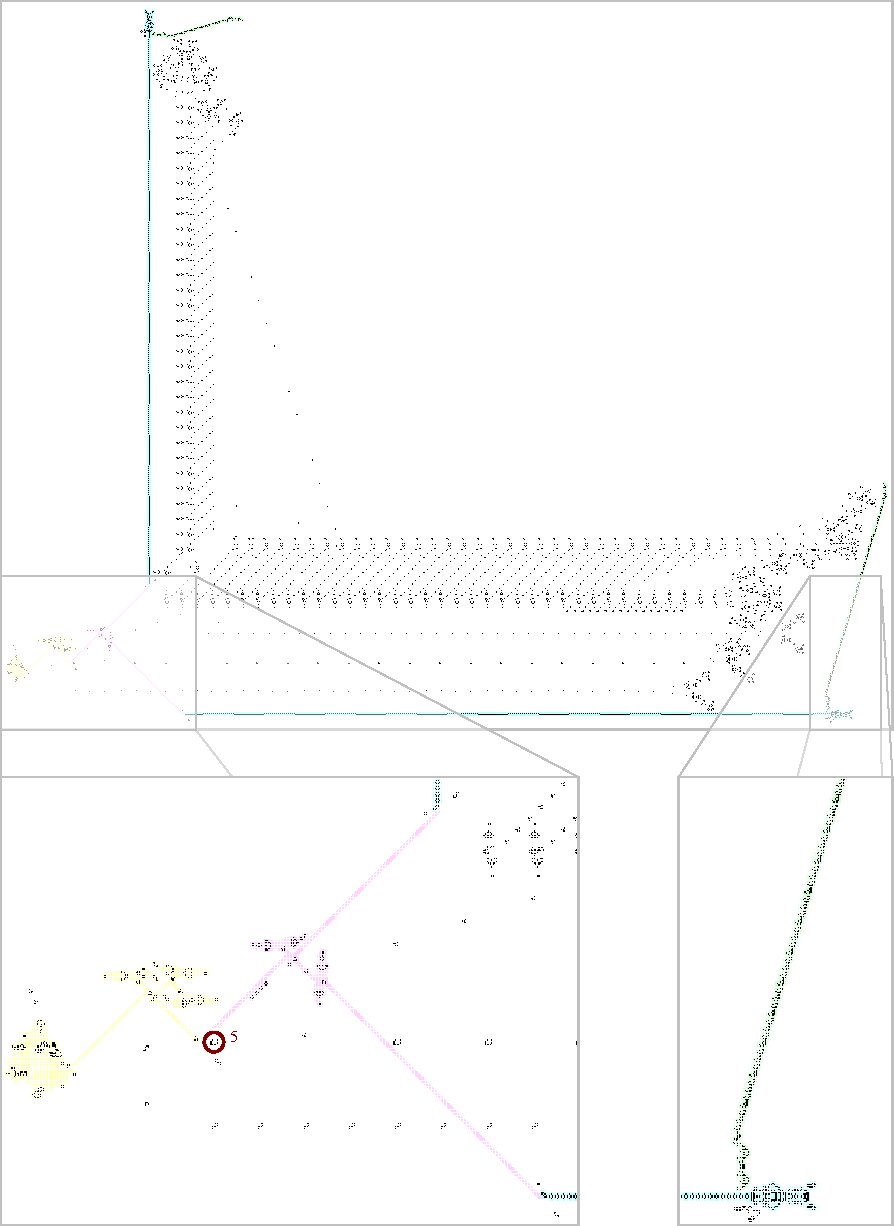
\includegraphics[width=0.925\textwidth]{glider_guns/fermat_prime.pdf}}
	\caption{A Fermat prime calculator that self-destructs and has bounded population if a sixth Fermat prime exists, but grows without bound otherwise. A caber tosser (highlighted in \bgbox{yellowback2}{yellow}) fires gliders at the lightweight spaceships that the primer creates corresponding to integers of the form $2^n+1$. If that LWSS is present (i.e., $2^n+1$ is prime) then the glider is reflected and destroys one of the four tubs to its northeast (they are destroyed by the known Fermat primes $5$, $17$, $257$, and $65{\thousep}537$). If another Fermat prime is found, the glider goes through a glider duplicator (highlighted in \bgbox{magentaback}{magenta}) and ignites two $4c/5$ beehive wicks that are laid by beehive puffers (highlighted in \bgbox{aquaback}{aqua}). Those wicks eventually cause two extensible $c/2$ spaceships (highlighted in \bgbox{greenpastel}{green}) to explode, blocking the primer.}\label{fig:fermat_primer}
\end{figure}

For spacing and timing reasons, this particular pattern starts with the Fermat prime $5$ (not $3$), and gliders corresponding to the Fermat primes $5$, $17$, $257$, and $65{\thousep}537$ each destroy a single tub near the southwest corner of the pattern. If a sixth Fermat prime is ever found, the resulting glider is fed into a glider duplicator that ignites both fuses and leads to the primer's self-destruction. However, such self-destruction will not happen until at least generation
\[
	120 \times 2^{2^{33}} \approx 1.16 \times 10^{2{\thousep}585{\thousep}827{\thousep}975},
\]
so evolving this pattern via computer software is not actually an effective method of checking whether or not a sixth Fermat prime exists.

While it is not possible to run this pattern long enough to see it self-destruct, we can force its self-destruction by manually erasing one or more of the glider-absorbing tubs at its southwest corner. If we erase all $4$ of those tubs, the glider corresponding to the Fermat prime $5$ almost immediately triggers the primer's self-destruction, whereas deleting a smaller number of tubs delays its self-destruction somewhat. If we remove just $1$ tub, the self-destruct fuse is ignited after roughly $8$~million generations (by the glider corresponding to the Fermat prime $65{\thousep}537$) and the primer finally stabilizes after roughly $21$~million generations.


%%%%%%%%%%%%%%%%%%%%%%%%%%%%%%%%
\section{Notes and Historical Remarks}\label{sec:glider_guns_history}
%%%%%%%%%%%%%%%%%%%%%%%%%%%%%%%%

Many of the ideas discussed early in this chapter were investigated right from the early days of Life. For example, many of the glider deletion tricks of Section~\ref{sec:glider_deletion} were already known in the early 1970s and were used to create the same period~$60$ gun that we constructed in Figure~\ref{fig:p60_gun}---see Figure~\ref{fig:lifeline_v11}. Indeed, the idea of encoding information in gliders and then using collisions between gliders to encode logical operations was already well-established at that time, and many useful interactions of this type were simply found by hand.

Other than guns resulting from these simple glider logic tricks though, not many new guns were found after the p$30$ Gosper glider gun and the p$46$ twin bees gun in the years following 1971. Bill Gosper made a p$1100$ gun sometime around 1984, Dean Hickerson constructed a p$94$ gun in 1990, Bill Gosper made a p$144$ gun in 1994 (see Exercise~\ref{exer:p144_gun_from_achim}), and David Buckingham had constructed guns of period~$44$ and $136+8n$ ($n \geq 1$), mostly based on his early work with Herschel tracks, by the early 1990s. However, progress in this area was relatively stagnant until he revealed Herschel track technology in full in 1996, and most of the earlier guns were so large and unwieldy that they were made almost instantly obsolete at that time.

% Really should be 2 paragraphs later. Just here for spacing reasons.
\begin{figure}[!htb]
	\centering
	\begin{minipage}[b]{0.46\textwidth}
		\centering
		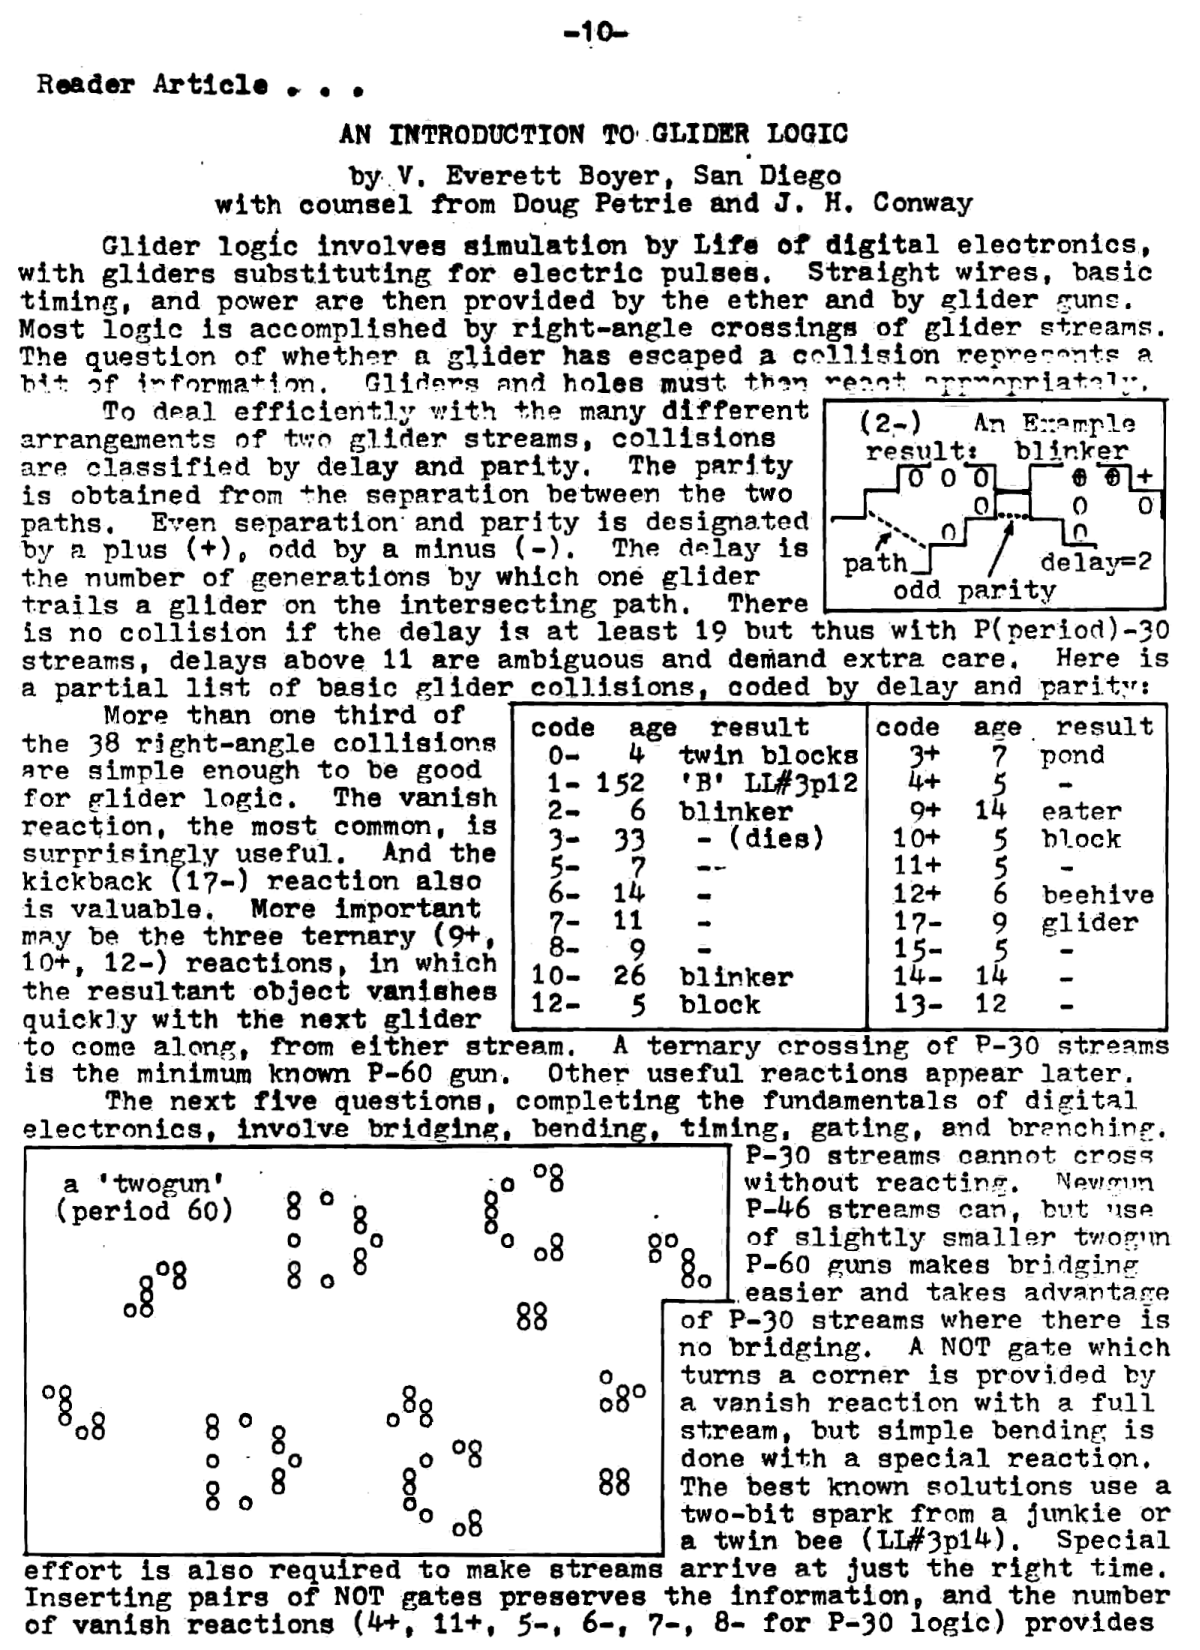
\includegraphics[width=0.8\textwidth]{glider_guns/lifeline_vol11.png}
		\caption{A page from the September 1973 issue (Volume 11) of \emph{Lifeline} that discussed glider logic and how it can be used to make a p$60$ glider gun (shown at the bottom left).}\label{fig:lifeline_v11}
	\end{minipage}\hfill
	\begin{minipage}[b]{0.5\textwidth}
		\centering
		\patternimglink{0.081}{p16_gun}
		\caption{A tightly packed p$16$ glider gun that uses a p$48$ gun (highlighted in \bgbox{magentaback}{magenta}) and two p$48$ glider insertions (highlighted in \bgbox{aquaback}{aqua} and \bgbox{greenpastel}{green}).}\label{fig:p16_gun}
	\end{minipage}
\end{figure}

After Herschel tracks hit the mainstream, which allowed for the systematic creation of glider guns of arbitrary large periods, a collaborative effort among many Life enthusiasts between then and 2003 (initiated by Dietrich Leithner and Peter Rott, and mainly led by Jason Summers and Karel Suhajda) produced explicit glider guns of all periods from $14$ to $1{\thousep}000$. The guns in this collection have since been shrunk down considerably via newer technology like Snarks and syringes, and at least a few of them are typically updated whenever a new sparky oscillator is discovered (as long as that oscillator can be used as a filter or reflector, anyway).\footnote{This collection of small glider guns is now being maintained by Adam P. Goucher as part of the Catagolue project. Up-to-date links to the smallest known guns of each period can be found at \httpsurl{catagolue.hatsya.com/census/b3s23/synthesis-costs/gun}.}

As a result of these repeated optimizations, most of the guns in this collection are now very cleverly and tightly packed---much moreso than the p$14$ gun that we constructed in Figure~\ref{fig:p14_gun}. Indeed, that gun had lots of empty whitespace that could be reduced by customizing the four glider insertion mechanisms that it uses, rather than using the exact same track for all four of them. For example, a particularly compact p$16$ gun is displayed in Figure~\ref{fig:p16_gun}.\footnote{However, this is not quite the smallest known p$16$ gun---see Exercise~\ref{exer:robs_p16_smaller_p16_gun}.} This gun uses a small p$24$ glider gun (one that is slightly smaller and newer than the one we saw in Figure~\ref{fig:p24_glider_gun}), which is then filtered to p$48$ by Rich's p$16$, and then sped up to p$16$ via two copies of the glider insertion reaction from Figure~\ref{fig:lwss_squish_pip}.

% Really should be 1 paragraph later. Just here for spacing reasons.
\begin{figure}[!htb]
	\centering
	\patternimglink{0.1425}{quadratic_filter}
	\caption{A \textbf{quadratic filter}, which reduces the growth rate of a gun quadratically. It works by using a pair of gliders (highlighted in \bgbox{aquaback}{aqua}) to pull a block from an ever-receding trail (highlighted in \bgbox{greenpastel}{green}), similar to the loaf-pulling reaction used in the recursive filter of Figure~\ref{fig:recursive_filter}. The rest of the device (highlighted in \bgbox{magentaback}{magenta}) extends the back end of the block trail. Here, the filter is attached to a p$90$ glider gun (highlighted in \bgbox{yellowback2}{yellow}), resulting in a sqrtgun.\index{sqrtgun} Constructed by Gabriel Nivasch in June 2006.}\label{fig:quadratic_filter}
\end{figure}

Patterns that decrease the asymptotic growth rate of a gun were known prior to the recursive filter of Figure~\ref{fig:recursive_filter}, but their effects were less pronounced. The first such pattern was a \textbf{quadratic filter},\index{quadratic filter} which is displayed in Figure~\ref{fig:quadratic_filter}. This pattern produces its $n$-th output glider after receiving its $n(n+1)/2$-th input glider,\footnote{This device relies on p$90$ circuitry, so the input gliders have to be aligned to that period.} and thus decreases the growth rate of glider guns quadratically. In particular, appending this pattern to a gun whose population in generation~$t$ is $\Theta(f(t))$ results in a gun with whose population is $\Theta(\sqrt{f(t)})$. For example, if we append $n$ of these quadratic filters in series after a gun whose population grows linearly (i.e., a ``standard'' glider gun), we get a gun whose population is $\Theta(t^{1/2^n})$.

The quadratic filter works by performing a block-pulling reaction whenever an input glider is received. Once a certain threshold is passed, the block is deleted, an output glider is released, and a farther-away block is created. If we rearrange the circuitry so that the location of the new block is pushed away \emph{every} time an input glider is received, rather than only when an output glider is produced, the filtering becomes even more pronounced. In fact, we get an \textbf{exponential filter}---a\index{exponential filter} pattern that can be attached to the output of a glider gun so as to decrease its growth rate exponentially.

% Really should be 1 paragraph later. Just here for spacing reasons.
\begin{figure}[!htb]
	\centering
	\patternimglink{0.136}{exponential_filter}
	\caption{An \textbf{exponential filter}, which reduces the growth rate of a gun exponentially, attached to a caber tosser (highlighted in \bgbox{yellowback2}{yellow}) so that its population in generation~$t$ is $\Theta\big(\log(\log(t))\big)$. It works via most of the same mechanisms as the quadratic filter of Figure~\ref{fig:quadratic_filter}, and was also constructed by Gabriel Nivasch in June 2006.}\label{fig:exponential_filter}
\end{figure}

The particular exponential filter that is displayed in Figure~\ref{fig:exponential_filter} produces its $n$-th output glider after receiving $5 \times 2^n - 4$ input gliders, so appending it to a gun whose growth rate is $\Theta(f(t))$ results in a gun with the slower growth rate $\Theta(\log(f(t)))$. For example, feeding the output of a caber tosser into this exponential filter, as in Figure~\ref{fig:exponential_filter}, results in a gun whose population in generation~$t$ is $\Theta\big(\log(\log(t))\big)$.

We could also apply several of these filters in sequence, producing guns with population
\[
	\Theta\big(\log(\log(\cdots (\log(t))))\big),
\]
where the logarithms are nested as many times as we like. However, even just a single usage of the recursive filter as in Figure~\ref{fig:recursive_filter_caber} results in a slower gun.


% EXERCISE: Make pattern with growth rate O(t^3/2) or O(t log^*t) (both easy, just attach guns we made here to a G-to-rake conduit). Earlier exercise: make G-to-rake conduit
% New p57: https://www.conwaylife.com/forums/viewtopic.php?f=2&t=3552&start=225#p128256
% Smallest p20 https://www.conwaylife.com/forums/viewtopic.php?p=85709#p85709

%%%%%%%%%%%%%%%%%%%%%%%%%%%%%%%%%
\section*{Exercises \hfill \normalfont\textsf{\small solutions to starred exercises on \hyperlink{solutions_glider_guns}{page \pageref{solutions_glider_guns}}}}
\label{sec:guns_exercises}
\addcontentsline{toc}{section}{Exercises}
\vspace*{-0.4cm}\hrulefill\vspace*{-0.3cm}\footnotesize\begin{multicols}{2}\vspace*{-0.4cm}\raggedcolumns\interlinepenalty=10000
	\setlength{\parskip}{0pt}\ifdefined\FORPRINTING\colorlet{ocre}{black}\else%
\fi
	%%%%%%%%%%%%%%%%%%%%%%%%%%%%%%%%%
	
	\begin{problemstar}\label{exer:p28_double} \probdiff{1}
		The glider collision in Figure~\ref{fig:glider_delete} can only be used to double the period of glider streams of period~$29$ or higher. Use the collision in Table~\ref{tab:2_glider_synth} that produces an eater~1 to double the period of a period~28 glider stream.
	\end{problemstar}

	
	\mfilbreak
	
	
	\begin{problem}\label{exer:gun_double_again} \probdiff{1}
		We used the reaction in Figure~\ref{fig:glider_delete} to turn two Gosper glider guns into a period~$60$ gun. Use that reaction multiple times to turn four Gosper glider guns into a period~$120$ gun.
	\end{problem}

	
	\mfilbreak
	
	
	\begin{problemstar}\label{exer:p322_gun} \probdiff{2}
		Use the reaction from Figure~\ref{fig:glider_delete6} to create a period~$322$ glider gun.
	\end{problemstar}
	
	
	\mfilbreak
	
	
	\begin{problem}\label{exer:duplicate_doubled_stream}
		The stream inverter-and-duplicator from Figure~\ref{fig:stream_inverter} is quite useful in situations where we want to duplicate a glider stream that took a lot of effort to create.\smallskip
		
		\begin{enumerate}[label=\bf\color{ocre}(\alph*)]
			\item \probdiff{1} Use three (not four!) Gosper glider guns and a single extra block to create a gun that fires two p$60$ streams of gliders.
			
			\item \probdiff{2} Use four (not six!) Gosper glider guns and two extra blocks to create a gun that fires three p$60$ streams of gliders.
		\end{enumerate}
	\end{problem}
	
	
	\mfilbreak
	
	
	\begin{problemstar}\label{exer:p80_gun_rich_p16} \probdiff{2}
		Use Rich's p16 (and potentially other sparkers as well) as a filter to turn the true-period~$20$ glider gun into a true-period~$80$ glider gun.
		
		\noindent [Hint: If you're lucky, you can get a single copy of Rich's p16 to delete \emph{two} consecutive gliders.]
	\end{problemstar}
	
	
	\mfilbreak
	
	
	\begin{problemstar}\label{exer:p4_glider_filter} \probdiff{2}
		We saw in Figure~\ref{fig:lwss_filter_tnosed_p4} that a filter can be used to double the period of any stream of lightweight spaceships with period $4n+2$ ($n \geq 3$). Explain why there cannot exist a filter capable of doubling the period of every stream of \emph{gliders} with period $4n+2$ ($n \geq 3$).
	\end{problemstar}


	\mfilbreak
	
	
	\begin{problem}\label{exer:p6_lwss_filter} \probdiff{2}
		Find an oscillator that can be used to double the period of any LWSS stream with period $6n+3$ ($n \geq 2$).
	\end{problem}
%	SOLUTION: p6 pipsquirter
%	x = 75, y = 20, rule = B3/S23
%	15bo2bo5b2o19bo2bo5b2o$b4o5b2o7bo3b4o4b4o5b2o7bo3b4o4b4o$o3bo3b2ob2o2b
%	o3bo3b2ob2o2bo3bo3b2ob2o2bo3bo3b2ob2o2bo3bo$4bo3b4o4b4o5b2o7bo3b4o4b4o
%	5b2o7bo$o2bo5b2o19bo2bo5b2o19bo2bo2$65bo$65bo2$63bo3bo$61b3obob3o$60bo
%	3b2o4bo$60bob2o2b2obobo$61bo2b2o2b2obo$62b2o2b2obobob2o$64bo2bobobob2o
%	$64b4ob2o$68bo$66bobo$66b2o!


	\mfilbreak
	
	
	\begin{problem}\label{exer:lwss_to_hwss_upgrade} \probdiff{2}
		We saw some ways of converting an LWSS into an MWSS and then an HWSS in Figure~\ref{fig:xwss_upgrade}. However, simpler conversions are possible with more loosely packed streams.\smallskip
		
		\begin{enumerate}[label=\bf\color{ocre}(\alph*)]
			\item Find a way of colliding a single glider with the back end of a lightweight spaceship so as to convert it into a heavyweight spaceship.
			
			\item What periods of HWSS streams can be made via this reaction?
		\end{enumerate}
	\end{problem}


	\mfilbreak
	
	
	\begin{problem}\label{exer:pseudo_xwss_gun_p18} \probdiff{4}
		Recall the reactions from Figures~\ref{fig:lwss_insertion_p18} and~\ref{fig:xwss_upgrade} that can be used to create p18 xWSS streams.\smallskip
		
		\begin{enumerate}[label=\bf\color{ocre}(\alph*)]
			\item Use (potentially multiple copies of) the LWSS insertion reaction to create a p18 LWSS gun.
			
			\item Use the LWSS-to-MWSS reaction to turn your LWSS gun from part~(a) into a p18 MWSS gun.
			
			\item Use the MWSS-to-HWSS reaction to turn your MWSS gun from part~(b) into a p18 HWSS gun (which is the smallest period possible for such a gun!).
		\end{enumerate}
	\end{problem}
	
	
	\mfilbreak
	
	
	% SOLUTION: http://conwaylife.com/forums/viewtopic.php?f=2&t=1651&start=50#p18616
	% Smallest currently known, mention in solution
	\begin{problem}\label{exer:smaller_G_to_LWSS} \probdiff{4}
		The conduit from Figure~\ref{fig:H_plus_G_to_WSS} can be used to create smaller stable glider-to-LWSS and glider-to-MWSS converters than we have seen so far.\smallskip
		
		\begin{enumerate}[label=\bf\color{ocre}(\alph*)]
			\item Use that conduit to build a smaller stable glider-to-LWSS converter than the one that we constructed in Figure~\ref{fig:glider_to_lwss_both}(b).
			
			[Hint: Be careful---do not use periodic reflectors like we did in Figure~\ref{fig:H_plus_G_to_WSS}, and make sure that the glider collides with the \emph{same} Herschel, rather than the \emph{next} one like in that figure.]
			
			\item Use that conduit to build a stable glider-to-MWSS converter.
		\end{enumerate}
	\end{problem}
	
	
	\mfilbreak
	
	
	\begin{problem}\label{exer:p28_adjust_29} \probdiff{3}
		Adjust the reflectors in the gun from Figure~\ref{fig:p14_pieces_p84} to create a gun that emits $2$ out of $3$ gliders in a p$29$ (instead of p$28$) stream.
	\end{problem}
	
	
	\mfilbreak
	
	
	\begin{problem}\label{exer:p156_adjust_lwss} \probdiff{2}
		Adjust the reflectors reaction from Figure~\ref{fig:p14_pieces_lwss} to make it work with Herschel streams of period~$180$ (instead of~$156$).
	\end{problem}
	
	
	\mfilbreak
	
	
	\begin{problem}\label{exer:jasons_p36_caterer} \probdiff{2}
		Show how to stabilize Jason's p$36$ (see Figure~\ref{fig:jasons_p36}) with caterers instead of jams.
	\end{problem}
	% SOLUTION:
	%x = 39, y = 22, rule = B3/S23
	%26bo$25bobo2$2o23bo$bo23b2o$bobo18b5o$2b2o18b2ob2o$14b2o9bo$13b2o$14b
	%2o$15bo$23bo$23b2o$24b2o$13bo9b2o$12b2ob2o18b2o$12b5o18bobo$12b2o23bo$
	%13bo23b2o2$11bobo$12bo!
	
	
	\mfilbreak
	
	
	\begin{problemstar}\label{exer:p21_glider_gun}
		A common method of creating a true-period glider gun is to replace a stabilizing component of a hassler, whose purpose it to absorb some debris, with another one that converts that debris into a glider. Consider the following period~$21$ B-heptomino hassler:\footnote{Found by David Raucci in August 2021. The period~$21$ gun that results from this exercise was found by Tanner Jacobi later on the same day.}
		\begin{center}
			\patternimglink{0.1}{exer_p21_oscillator}
		\end{center}
		
		\begin{enumerate}[label=\bf\color{ocre}(\alph*)]
			\item \probdiff{1} If one of its boats is removed, what common object forms at the edge of the oscillator, causing it to self-destruct?
			
			\item \probdiff{3} Show how the following period~$7$ oscillator can be used to convert the object from part~(a) into a glider, thus creating a true-period~$21$ glider gun:
			\begin{center}
				\patternimglink{0.1}{exer_p7_oscillator}
			\end{center}
			
			\item \probdiff{2} Create a true-period $42$ glider gun.
		\end{enumerate}
	\end{problemstar}


	\mfilbreak
	
	
	\begin{problem}\label{exer:p56_gun_smaller} \probdiff{2}
		Construct a true-period 56 gun that is smaller than the one from Figure~\ref{fig:p56_gun}.
		
		\noindent [Hint: Just add a filter to some other gun.]
	\end{problem}
	% SOLUTION: Filter the p28 gun with a blocker.
	
	
	\mfilbreak
	
	
	\begin{problem}\label{exer:smaller_p14_gun} \probdiff{4}
		By using (multiple copies of) the p28 glider gun from Figure~\ref{fig:p28_glider_gun}, construct a period~14 glider gun that is smaller than the one that we built in Figure~\ref{fig:p14_gun}.
	\end{problem}
	% SOLUTION: Posts right after https://www.conwaylife.com/forums/viewtopic.php?t=&p=115869#p115869
	
	
	\mfilbreak
	
	
	\begin{problem}\label{exer:p54_fold_corners} \probdiff{3}
		The p$56$ glider gun displayed in Figure~\ref{fig:p56_gun} uses three reflectors at its top and at its bottom, instead of just one, to make it bounding box slightly smaller. You can similarly ``fold in'' the top and bottom corners of some other guns to make their bounding boxes smaller.
		
		\begin{enumerate}[label=\bf\color{ocre}(\alph*)]
			\item Modify the p$54$ glider gun from Figure~\ref{fig:p54_gun} so that its bounding box has at least $300$ fewer cells in it.
			
			\item Modify the p$55$ glider gun from Figure~\ref{fig:p55_gun} so that its bounding box has at least $700$ fewer cells in it.
		\end{enumerate}
	\end{problem}


	\vspace*{1cm}
	\mfilbreak
	
	
	\begin{problem}\label{exer:p51_49_guns} \probdiff{3}
		The following reaction converts $2$ input gliders into $3$ output gliders:\footnote{This base reaction was found by ``hotcrystal0'' and ``wwei'' in November 2021, and the resulting p51 and p49 guns were first constructed shortly thereafter by Luka Okanishi and Tanner Jacobi, respectively.}
		
		\begin{center}
			\patternimglink{0.1}{exer_p51_reaction}
		\end{center}
		
		\begin{enumerate}[label=\bf\color{ocre}(\alph*)]
			\item Use (potentially multiple copies of) this reaction to create a true-period $51$ gun.
			
			\item Replace the p$3$ sparkers with the following p$7$ sparker, and then create a true-period $49$ gun:
			
			\begin{center}
				\patternimglink{0.1}{exer_p7_dot_spark}
			\end{center}
		\end{enumerate}
	\end{problem}


	\mfilbreak
	
	
	\begin{problem}\label{exer:H_G_reacs_58_61} \probdiff{1}
		Determine the repeat times of the four conduits from Figure~\ref{fig:H_G_reacs_58_61}.
	\end{problem}
	
	
	\mfilbreak
	
	
	\begin{problemstar}\label{exer:p50_glider_stabilize} \probdiff{3}
		Another method of stabilizing one side of the pi-heptomino reaction used in the true-period~$44$ and~$50$ glider guns is displayed below.
		\begin{center}
			\patternimglink{0.1}{exer_p50_glider_stabilize}
		\end{center}
		\noindent Use this reaction to create a true-period~$50$ glider gun that is different than the one from Figure~\ref{fig:p50_true_gun}. In particular, use two mirror-image copies of the glider-extracting conduit and then feed one of those gliders back into the reaction via...\smallskip
		
		\begin{enumerate}[label=\bf\color{ocre}(\alph*)]
			\item two Snarks.
			
			\item two bumpers (what is the only known bumper period that works with period~$50$ mechanisms?).
		\end{enumerate}
	\end{problemstar}


	\mfilbreak
	
	
	\begin{problem}\label{exer:fx77_extract_other_osc} \probdiff{2}
		Show how to extract a glider from an Fx77 conduit like we did in Figure~\ref{fig:fx77_extract} via the following oscillators:\smallskip
		
		\begin{enumerate}[label=\bf\color{ocre}(\alph*)]
			\item a unix (p$6$),
			
			\item a pentadecathlon (p$15$), and
			
			\item Beluchenko's p$7$ (Figure~\ref{fig:sparky_p7}).
		\end{enumerate}
	\end{problem}
	% SOLUTION: https://conwaylife.com/wiki/Fx77
	
	
	\mfilbreak
	
	
	\begin{problem}\label{exer:p61_gun_reflection_no_60} \probdiff{2}
		Explain why the method of separating the two close glider streams in the p$61$ gun from Figure~\ref{fig:p61_gun} (by reflecting one of the gliders off of the corner of an L112 conduit) does not work at p$58$, p$59$, or p$60$, despite L112 having a repeat time of~$58$ generations.
	\end{problem}
	% SOLUTION: eater 2 only fast enough at p61 and higher. Can replace with another eater (to get lower repeat time, like eater 5 variant), but then interferes with passing gliders
	
	
	\mfilbreak
	
	
	\begin{problem}\label{exer:2_lane_slide_gun} \probdiff{3}
		Use the reaction from Figure~\ref{fig:synchronized_block_reflector_4} to create a slide gun that fires gliders separated by $2$ lanes (instead of $4$ lanes, like the slide gun from Figure~\ref{fig:slide_gun}).
	\end{problem}
	
	
	\mfilbreak
	
	
	\begin{problem}\label{exer:slide_gun_honey_farm}\index{honey!farm} \probdiff{3}
		Slide guns can be made to work by pushing any stable object, not just a block. Use the following reactions\footnote{Both found by Jason Summers in 1999. The reaction in part~(a) was used in the quadratic and exponential filters of Figures~\ref{fig:quadratic_filter} and~\ref{fig:exponential_filter}.} to create slide guns:\\[0.05cm]
		
		\begin{enumerate}[label=\bf\color{ocre}(\alph*)]
			\item \raisebox{-\height+\ht\strutbox}{\patternlink{exercise_honey_farm_pusher}{\vcenteredhbox{\patternimg{0.1}{exercise_honey_farm_pusher_0}} \vcenteredhbox{\genarrow{51}} \vcenteredhbox{\patternimg{0.1}{exercise_honey_farm_pusher_1}}}}\\[0.1cm]
			
			\item \raisebox{-\height+\ht\strutbox}{\patternlink{exercise_beehive_pusher}{\vcenteredhbox{\patternimg{0.1}{exercise_beehive_pusher_0}} \vcenteredhbox{\genarrow{33}} \vcenteredhbox{\patternimg{0.1}{exercise_beehive_pusher_1}}}}\\[0.1cm]
		\end{enumerate}
	\end{problem}
	% SOLUTION FOR (a) is contained in here:
	%x = 263, y = 178, rule = B3/S23
	%186bo2b2o$186bo2bo$186bo11$168b2o$169b2o$168bo3$163b2o$164b2o22bo$163b
	%o25bo$187b3o$177b3o$179bo$178bo12$145b2o$146b2o$145bo3$140b2o$141b2o$
	%140bo2$154b3o$156bo$155bo$211bo$212bo$210b3o9$122b2o$123b2o$122bo2$
	%188b2o$117b2o69bo$118b2o$117bo2$131b3o$133bo6b2o$132bo7bo$77b2o$77bo4$
	%244bo$29b2o211b2o$29bo41bo5bo165b2o$70b3o3b3o109bo7bo$69b2o2bobo2b2o
	%107b4o3b4o$69bo3bobo3bo107bo3bobo3bo$69bob2o3b2obo19b2o41b2ob2o41bo2bo
	%bo2bo$69b2o7b2o20b2o40b2ob2o41b3o3b3o$99bo42b2ob2o$140bob2ob2obo$140b
	%3o3b3o$22b3o3b3o63b2o45bo5bo$22bo2bobo2bo64b2o$22bo7bo63bo$195b2o9bo2b
	%2o$108b3o62bo21bo10bo2bo$110bo58b2o2bo32bo$109bo58bo5bo$167b2o2bobo$
	%168b2o3bo$169b3o2$77b2o90b3o$77bo59b3o3b3o22b2o3bo$58b2o3bo73bo2bobo2b
	%o15b2o4b2o2bobo$58b3obob2o71bo7bo5bo9bo6bo5bo$58b3o4bo86b2o15b2o2bo$
	%61bo3bo85b2o20bo14b2o$27bobo32b3o3bo120b2o$28b2o38b2o6b2o110bo$28bo33b
	%3o3b2o7b2o127b2o$61bo3bo10bo130b2o$43b2o13b3o4bo117b2o21bo$43bo14b3obo
	%b2o118b2o$58b2o3bo7b2o110bo$72b2o$71bo125b3o$199bo$18b2obo3bob2o56b3o
	%47b2o17b2o42bo$19b3o3b3o11bo47bo48bo17bo$20bo5bo13b2o44bo46b3o19b3o$
	%39b2o92bo23bo5$17b2o17b2o$18bo17bo$15b3o19b3o134bo$15bo23bo135b2o$23b
	%3o3b3o108b2obo3bob2o23b2o37bo$22bo2bo3bo2bo108b3o3b3o62b2o$22b2obo3bob
	%2o56bo52bo5bo63bobo$88b2o$88bobo102b2o$160b2o29b2ob2o14b2o$161b2o28bo
	%2bo15bo$48b2o110bo30bo2bo$49b2o141b2o$48bo$148b2o15b2o25b2o$62b3o83bo
	%16bo25bo2bo$64bo16b4o78bobo17b2o6bo2bo15b2o2b2o$63bo17bo2b2o6b2o69b2o
	%18bo7b2ob2o14bo4bo7b2obo$82bo2b2o5bo100b2o20bobo4bob2ob2o$82bo2bo73b2o
	%55b2o4bo3b2o$83b2o74bo64bo$170b2o51b2o$30b2o15b2o34b2o84bo2b2o11b2o20b
	%2o$30bo16bo34bo2bo32b2o9b4o35b6o11bo23bo$38b2o5bobo17b2o15bo2b2o31bo
	%10b2obo37b4o20b2o10b2o2bo35b3o$38bo6b2o18bo15bo2b2o46bo20b2o39bo12bo2b
	%o33bo4bo11b2o$81b4o45b2o20bo2bo52bobo18bo14bo5bo10bo$151b2o2bo52b2o18b
	%2o6bo12bo$130b2o20bo2bo14b4o53b3obo3b2o10b2o$54b3o55bo19bo20bo14b6o34b
	%2o16b2o7bobo$15b2o36bo4bo8b2o42b2o16b2obo36bo2b2o34bobo16b2o18b2o$14bo
	%2bo34bo5bo8bo35b2o6bobo15b4o20bo16b2o35bo2bo17bo20bo$13b2o2bo35bo50bo
	%47bo2bo50b2o2bo33bo5bo$14bo2bo14b2o20b2o48bobo44b2o2bo53bo18bo15bo4bo$
	%15bo9b2o4bo2b2o69b2o45bo2bo51b2o18b2o17b3o$26b2o2b6o18b2o97b2o8b2o61b
	%2o$15bo9bo6b4o17bo109bobo61b3obo$14bo2bo34bo5bo106bo50b2o10b2o$2o11b2o
	%2bo35bo4bo41b2o63b2o48bobo11bo$o13bo2bo36b3o26b2o15bobo112bo$15b2o15b
	%4o47bo18bo36b3o8b2o62b2o$30b6o64b3o20b2o16bo8bo$31bo2b2o78bo7b2o17bo$
	%32b2o11b2o66b2o9bo15bo$45bobo64b2o$47bo52b3o10b2o25bo$47b2o53bo38bo$
	%100bobo38bo$100b2o37b3o$113b2o$112b2o$113b2o$105b2o7bo$104bobo$104bo$
	%103b2o!
	% SOLUTION FOR (b) -- should probably be rebuilt using an MWSS-creating mechanism we have actually seen before:
	%x = 124, y = 91, rule = B3/S23
	%101b2o14b2o$101b2o14b2o5$100b3o$100b3o$99bo3bo2$98b2o3b2o12b3o$116bo3b
	%o$115bo5bo$115bo5bo$118bo$98b3o15bo3bo$40b2o60b2o13b3o$39bobo60b2o14bo
	%$29b2o7b3o12bo49b2o$29b2o6b3o8b2o3b4o44bobo$38b3o8b2o3b4o5b2o36b2o16b
	%3o$39bobo2b2obob2o3bo2bo5b2o54b3o$40b2o2b2obobo4b4o60bo3bo$23bo22b2obo
	%3b4o39b2o3b2o9bobo$21bobo29bo42b2o3b2o9b2o3b2o3b2o$12bo7bobo11b2o77bo$
	%11b2o6bo2bo11b2o62b3o$10b2o4b2o2bobo16bo58b3o$2o7b3o4b2o3bobo13b2o60bo
	%$2o8b2o4b2o5bo14b2o$11b2o73bo$12bo73bo$24bo60bobo$25bo60bo9b2o$23b3o
	%60bo10bo21b2o$30bobo53bo7b3o22b2o$29b3o54bo7bo$27b5o53bobo$27bobo56bo
	%10bobo$29bo56bo10b2o$29b2o67bo$110bo$108bo3bo3b2o$25bo11bo29bo29bo15bo
	%bo2bo$24bobo8bo3bo25bo3bo25bo3bo8bo4bo2b2o$23bo3bo12bo29bo29bo8b5o$23b
	%o3bo7bo4bo24bo4bo24bo4bo$23bo3bo8b5o25b5o13b2o10b5o$23bo3bo57b2o$23bo
	%3bo56bo$23bo3bo8b2o$24bobo40bo$25bo9bo12bo16b3o$36bo8b4o15bo$32b2o10b
	%4o9b2o5b2o19bo$32bobo9bo2bo9b2o24b3o$33b3o8b4o5bo28bo$34b3o8b4o4bo28b
	%2o$33b3o12bo$25b2o5bobo44bo$24bobo5b2o45bo$24bo55bo$23b2o44b2o$70b2o$
	%60b5o4bo7b2o3b2o$59bob3obo11bo5bo$60bo3bo$61b3o10b2o2bo3bo$62bo10b2o4b
	%3o$63b2o10bo$63bobo$63bobo$64bo3$61b2obob2o10bo$61bo5bo8b2ob2o$62bo3bo
	%$63b3o9bo5bo2$75b2obob2o6$64b2o$64b2o2$77b2o$77b2o!
	
	
	\mfilbreak
	
	
	\begin{problem}\label{exer:simkin_glider_gun_smaller_slide} \probdiff{3}
		Use the small p$120$ glider gun from Exercise~\ref{exer:simkin_glider_gun} to rebuild the slide gun from Figure~\ref{fig:slide_gun} within an $85 \times 70$ bounding box.
	\end{problem}
	% SOLUTION
	%x = 64, y = 80, rule = B3/S23
	%52bo$50b3o$8b2o39bo$8b2o39b2o3$11b2o$11b2o31b3o$46bo6b2o5b2o$8b2o35bo
	%7b2o5b2o$8b2o$2o33bo20b2o$bo32bobobo17b2o$bobo32bo2bo$2b2o$35bo$35bo$
	%35b2o$9bo2bo22bo3bo$7b4o18b2o4bob2o$13bo15b2o4b3o$7b2o2b2o2$11b2o$12b
	%2o$8bo2b2o$19b2o$19b2o10bo$29bobo$16b2o12b2o$16b2o7bo$25b3o$28bo12b2o$
	%19b2o6b2o13bo$19b2o21bobo7bo$43b2o5bobo$33bobo12b2o$34b2o12b2o12b2o$
	%34bo13b2o12b2o$50bobo$30bo21bo$29b3o9bo$28b5o8b2o$27b2o3b2o6bobo3$31bo
	%$19b2o10bo$19b2o$27b2o$28bo$16b2o7b3o$16b2o7bo2$19b2o$19b2o3$59b2o$59b
	%2o2$20bo$17b5o$16bo2$17bo3bo$18b3o$2b2o$bobo$bo$2o$8b2o$8b2o2$11b2o$
	%11b2o3$8b2o$8b2o!
	
	
	\mfilbreak
	
	
	\begin{problem}\label{exer:edge_shoot_30n}
		The device below\footnote{Found by Arie Paap and Tanner Jacobi in late 2018 in a period~$30n$ ($n \geq 2$) form, and adjusted to the period~$5n$ form shown here in late 2019.} can be attached to the output of any gun with period~$5n$ ($n \geq 8$) to create an edge-shooting gun of the same period:
		\begin{center}
			\patternimglink{0.12}{exercise_edge_shoot_30n}
		\end{center}
		
		\begin{enumerate}[label=\bf\color{ocre}(\alph*)]
			\item \probdiff{3} Use this reaction to create an edge-shooting p$240$ gun.
			
			\item \probdiff{4} Use $10$ copies of the gun from part~(a) (and perhaps the p$120$ glider gun from Exercise~\ref{exer:simkin_glider_gun}) to rebuild the slide gun from Figure~\ref{fig:double_slide_gun} in a much smaller way. In particular, this edge shooter lets you avoid using the glider insertion mechanism from Figure~\ref{fig:lwss_reflect_glider}.
		\end{enumerate}
	\end{problem}
	
	
	\mfilbreak
	
	
	\begin{problem}\label{exer:slide_gun_hd} \probdiff{4}
		Create a slide gun that fires gliders separated by just $1$ lane.
		
		\noindent [Hint: This is tricky! The reactions like Figure~\ref{fig:synchronized_block_reflector_4} that move a block $1$~cell diagonally result in slide guns with a separation of $2$~lanes.]
	\end{problem}
	% Solution: need 2 separate firing reactions. Fire, then move by (0,1), then fire, then move by (1,0), repeat
	
	
	\mfilbreak
	
	
	\begin{problem}\label{exer:slide_gun_no_slide} \probdiff{2}
		Create a ``slide'' gun that fires $7$~gliders at a block so as to create a perpendicular glider without moving the block at all. That is, create a slide gun that doesn't slide.
	\end{problem}
	% SOLUTION: just remove 3 gliders from {fig:double_slide_gun}
	
	
	\mfilbreak
	
	
	\begin{problem}\label{exer:triple_slide_gun} \probdiff{4}
		Create a slide gun that fires $3$~gliders on each of its output lanes (instead of $2$, like in Figure~\ref{fig:double_slide_gun}).
		
		\noindent [Hint: Using an edge-shooting gun like the one from Exercise~\ref{exer:edge_shoot_30n} will help keep the size of your slide gun down.]
	\end{problem}


	\mfilbreak
	
	
	\begin{problem}\label{exer:four_lane_gun_smaller} \probdiff{3}
		Decrease the bounding box of the four-lane gun from Figure~\ref{fig:armless_4_lane_gun} so that it no larger than $275 \times 275$, by using Snarks to wrap the glider loops around like we did in Figures~\ref{fig:armless_monochrome_cordership_gun} and~\ref{fig:armless_cordership_gun}.
	\end{problem}
	% SOLUTION: https://conwaylife.com/forums/viewtopic.php?p=85842#p85842
	
	
	\mfilbreak
	
	
	\begin{problem}\label{exer:armless_basics}
		Armless glider production is a useful and highly adjustable mechanism, but some adjustments have consequences that may not be intuitively obvious.\smallskip
		
		\begin{enumerate}[label=\bf\color{ocre}(\alph*)]
			\item \probdiff{2} What behavior appears if you try to produce perpendicular output gliders via two loop guns whose periods differ by a multiple of 8?
			% SOLUTION: the output glider lane(s) drift in one direction or the other, eventually reaching and probably destroying one of the loop guns.
			
			\item \probdiff{4} Make a design for a ``drifting'' armless gun that would allow loop guns of different periods, but avoid the problem that was alluded to in part~(a).
			% SOLUTION: One option would be to adjust the loop guns' periods to particular multiples of 8, so that there's some number P = N*{gun1 period} = (N+1)*{gun2 period}. Then add an additional period-P gun that suppresses one signal from gun #2, producing a period-P ``scanning'' or ``strobing'' effect.
		\end{enumerate}
	\end{problem}
	
	
	\mfilbreak
	
	
	\begin{problem}\label{exer:armless_tee}
		In Section~\ref{sec:armless}, we only constructed armless guns that fire slow salvos. However, we can also construct ones that fire synchronized salvos.\smallskip
		
		\begin{enumerate}[label=\bf\color{ocre}(\alph*)]
			\item \probdiff{4} Use (several copies of) the p387 loop gun displayed below on the left, along with the H-to-2G conduit that we used in our tee-based armless guns, to create a $4$-consecutive-lane armless gun that fires the tight arrangement of gliders displayed below on the right.\\[-0.6cm]
			
			\begin{center}
				\begin{minipage}[t]{.575\linewidth}\vspace{0pt}
					\centering \patternimglink{0.1}{exercise_herschel_tee_387_loop}
				\end{minipage} \hfill %
				\begin{minipage}[t]{.38\linewidth}\vspace{0pt}
					\centering \patternimglink{0.14}{exercise_herschel_tee_4_gliders}
				\end{minipage}
			\end{center}
		
			\item \probdiff{2} Adjust your gun from part~(a) so that it fires that configuration of gliders with period 129.
			
			\noindent [Hint: $129 \times 3 = 387$.]
			
			\item \probdiff{3} Adjust your gun from part~(a) so that it fires that configuration of gliders with period 87 (which is minimal).
			
			\noindent [Hint: $387+6 \times 8 = 435 = 87\times5$, so first adjust each loop to be 6fd bigger.]
		\end{enumerate}
	\end{problem}
	% SOLUTIONS: patterns are posted at  https://conwaylife.com/forums/viewtopic.php?p=86064#p86064


	\mfilbreak


	\begin{problem}\label{exer:armless_tee_decrease_repeat_time}
		In this exercise, we explore some methods that can be used to decrease the repeat time of an armless gun.\smallskip
		
		\begin{enumerate}[label=\bf\color{ocre}(\alph*)]
			\item \probdiff{3} The tee-based armless Cordership gun of Figure~\ref{fig:armless_monochrome_cordership_gun} has already been adjusted to close to its recipe's minimum repeat time of $2{\thousep}061$ generations. Explain how additional loop guns could be added to allow a repeat time of less than $2{\thousep}000$ generations.
			% SOLUTION: Add more loop guns: Wherever a 74-tick limitation appears, move one of the gliders involved to a separate pair of loop guns.
			
			\item \probdiff{5} How could the repeat time of this gun be reduced \emph{without} increasing the number of loop guns?
			% SOLUTION: There are some long stretches of same-color gliders in both salvos making up the Cordership glider-pair recipe. For the glider pairs that build blocks, there are alternate recipes (e.g., the mirror image of the current recipe) that can switch one or both gliders to a different color.
			%Might not need a figure for this, but here's some RLE just in case. The left-side glider is a different color in these two recipes:
			% x = 34, y = 9, rule = LifeHistory
			% 4.2D23.2D$3.B2DB22.2DB$2.5B22.2B2C$.4B.3B18.4BCBC$3CB2.4B16.4B.CB$2BC
			% 4.4B14.2C3B$.C6.2B2C12.CBCB$9.BCBC12.BC$10.CB!
			% ... and if you take the mirror image of the right-side recipe, both gliders change colors.
		\end{enumerate}
	\end{problem}
	
	
	\mfilbreak
	
	
	\begin{problem}\label{exer:slow_glider_pairs_cordership_armless}
		In a tee-based armless gun that implements 2-directional slow synthesis, the gliders in the loop guns are synchronized in groups of four. Adjustments to the four gliders in a group can make a collision happen in a different place, or at a different time.\smallskip
		
		\begin{enumerate}[label=\bf\color{ocre}(\alph*)]
			\item \probdiff{2} Find a case where a glider follows another one by just 74 generations in the tee-based armless Cordership gun of Figure~\ref{fig:armless_monochrome_cordership_gun}. Then find the other three gliders that are synchronized with that glider, and delay all four gliders by one generation. What happens?
			% SOLUTION: Most likely the recipe will still work, but one part of it will be constructed one tick more slowly than before. Occasionally, if the changed position causes a conflict with other gliders, the recipe will fail.
			
			\item \probdiff{2} Return the four gliders to their original positions, and instead of delaying them all, advance them all by one generation. What happens?
			% SOLUTION: The other three gliders in the group will generally have much plenty of space in front of them, but the first glider's 74-tick spacing is a limiting factor that prevents that particular collision from occurring any sooner in the construction recipe. Attempting to advance the 74-tick following glider will cause a failure in the syringe conduit, the next time that glider attempts to pass through.
			
			\item \probdiff{3} Find the four gliders that collaborate to produce the southernmost block in the Cordership seed. How would you move those gliders to build the block two cells directly south of its current position, or one cell directly southeast or southwest?
		\end{enumerate}
	\end{problem}


	\mfilbreak
	
	
	\begin{problem}\label{exer:multicolor_armless}\index{NW31}
		It is somewhat easier to change the period of a multicolor armless gun than the monochrome one, since they have fewer glider loops to adjust. The multicolor armless Cordership gun of Figure~\ref{fig:armless_cordership_gun} has period $5{\thousep}603$.\smallskip
		
		\begin{enumerate}[label=\bf\color{ocre}(\alph*)]
			\item \probdiff{3} A syringe followed by NW31 (i.e., the conduit of Figure~\ref{fig:H_to_2G}) makes a stable glider reflector. Add one of these reflectors to one of the loop guns from the multicolor armless Cordership gun. How does its period change?
			
			\noindent [Hint: Start by moving some Snarks a long distance away to make space.]
			% SOLUTION: adding a syringe+NW31 component similar to the ones in the Cordership guns, will add 3 ticks (mod 8) to the period.  That is, if the gun period is N before adding a syringe+NW31, then after the addition it will be possible to adjust the new period to N+3.
			
			\item \probdiff{3} Adjust that glider loop so that it has period $2^{13} = 8{\thousep}192$.
			
			[Hint: You cannot just adjust the trombone slides, since the mod-$8$ length of that loop is not right. Either add more syringe $+$ NW31s or add another reflector from Table~\ref{tab:conduit_phase_changers}.]
			% SOLUTION: a chain of seven syringe+NW31s will allow for a p2603+7*3+8N gun, which can be adjusted to period 8192.
			
			\item \probdiff{4} Make the same adjustments to the other three loop guns to produce a working period~$8{\thousep}192$ Cordership gun.
		\end{enumerate}
	\end{problem}
	
	
	\mfilbreak
	
	
	\begin{problem}\label{exer:caber_tosser_rewind} \probdiff{2}
		Explain why we cannot rewind the caber tosser from Figure~\ref{fig:caber_tosser_0} so that the triggering glider in aqua is traveling northwest before it is reflected by the caber tosser.
	\end{problem}
	
	
	\mfilbreak
	
	
	\begin{problem}\label{exer:caber_tosser_stationary} \probdiff{3}
		Construct a caber tosser that uses the same Cordership and glider bouncing off of it as in Figure~\ref{fig:caber_tosser_0}, but uses stationary circuitry (e.g., syringes and Herschel conduits) in place of the glider guns.
	\end{problem}
	
	
	\mfilbreak
	
	
	\begin{problem}\label{exer:caber_tosser_different_speeds} \probdiff{2}
		If a caber tosser makes use of a receding spaceship with speed $s_1$ (instead of a Cordership) and bouncing spaceship with speed $s_2$ (instead of a glider), what is the ratio of the gaps between the gliders that it emits? For example, in the caber tosser of Figure~\ref{fig:caber_tosser_0} we had $s_1 = c/12$, $s_2 = c/4$, and a ratio of $2$ (each glider took twice as long to be emitted as the previous one).
	\end{problem}
	% SOLUTION: $(s_2+s_1)/(s_2-s_1)$
	
	
	\mfilbreak
	
	
	\begin{problem}\label{exer:sqrtgun_standard} \probdiff{4}
		Rebuild the sqrtgun from Figure~\ref{fig:sqrtgun} without any Herschel tranceivers---use syringes (and other ``modern'' Herschel conduits) instead.
	\end{problem}
	
	
	\mfilbreak
	
	
	\begin{problem}\label{exer:construct_fermat_primer} \probdiff{2}
		Construct a gun that emits lightweight spaceships corresponding to Fermat primes (much like the primer itself emits lightweight spaceships corresponding to all primes), rather than a pattern that self-destructs if it finds a sixth Fermat prime like the one we made in Figure~\ref{fig:fermat_primer}.
	\end{problem}
	
	
	\mfilbreak
	
	
	\begin{problem}\label{exer:fermat_beehive_puffer} \probdiff{2}
		The beehive puffer that is used at the bottom-right and top-left of the Fermat prime calculator (see Figure~\ref{fig:fermat_primer}) is displayed below.
		
		\begin{center}
			\patternimglink{0.1}{fermat_beehive_puffer}
		\end{center}
		
		\noindent This puffer still works even if the cells highlighted in \bgbox{aquaback}{aqua} are deleted. What is their purpose in the Fermat prime calculator?
	\end{problem}


	\mfilbreak
	
	
	\begin{problem}\label{exer:mersenne_primer}\index{Mersenne prime} \probdiff{3}
		Modify the Fermat prime calculator of Figure~\ref{fig:fermat_primer} so that it computes \textbf{Mersenne primes}: primes of the form $2^n - 1$ for some integer $n$.
	\end{problem}
	% SOLUTION: Example solution given here: http://www.njohnston.ca/2009/08/generating-sequences-of-primes-in-conways-game-of-life/
	% http://www.conwaylife.com/patterns/mersenneprimecalculator.rle
	
	
	\mfilbreak
	
	
	\begin{problem}\label{exer:robs_p16_smaller_p16_gun}
		Recall the small p$16$ oscillator from Figure~\ref{fig:rob_p16} called Rob's p$16$.\smallskip
		
		\begin{enumerate}[label=\bf\color{ocre}(\alph*)]
			\item \probdiff{2} Show how Rob's p16 can be used to filter a p$24$ LWSS stream, creating a p$48$ stream.
			
			\item \probdiff{2} What LWSS stream periods can be filtered by Rob's p16? % $16n+8$ for any $n \geq 1$ (same as Rich's p16)
			
			\item \probdiff{4} Use the filtering reaction from part~(a) to reduce the bounding box of the p$16$ glider gun that we saw in Figure~\ref{fig:p16_gun} by at least $2$ rows or columns.
		\end{enumerate}
	\end{problem}
	% SOLUTION:
	%x = 156, y = 154, rule = B3/S23
	%5b2ob2o5bo3bo5b2ob2o63b2o$5b2obo5b2o3b2o5bob2o61b3obo19b2o4b2o3b2o4b2o
	%b2o$8bob2o11b2obo63bo4bo12b2o5bobo3b2o3b2o3bobob2o$8bo6b2ob2o6bo62bobo
	%bob2o10bo2bob2obo5bobobobo5bo$9b2o13b2o55b2o7bo2bo13bo2bobo2bo2bo11bo
	%2bo$3bobo6bo2b2ob2o2bo27b2o28bo2bo2b4o2b2ob2o3b2o2b2ob4o2bo2bo15bo$b3o
	%b3o5b3o3b3o27bob3o20b2o4b3o2b7obobo4b2o2bobo4b2o7bob2ob2obo7bobo$o7bo
	%5bo5bo8bo19bobo2bo19bo8b9o3bo10bob2o10bo2bobo2bo5b3ob3o$ob6o20bobo4bo
	%12b2o2b2obo20bo5bo10b2o3b4o3bob2ob3o7b3o3b3o4bo7bo$7bo20bobo2b3o15bob
	%2o2bo4b2o11b4o3b2o14bo2bo2bo5bo2bo19b6obo$bo2bo22b2obobo10b2o3b2obo7bo
	%bo2bo9bo4bo24b5obo2bo20bo4b2o$2bobo2b2o10bobo4bo3bobob2o7b2o4bobo10b3o
	%9b5obo30bob2o18b2o3bo$3bo3b3o10bo4b3ob2o4bo13bobobo6b2o10b2o2bobobo8b
	%4o5bo5b2o3bobo4bo4bo10bobo2bobo$7b3o4bo10b3o4b3o8b4o3bo3b6o2bo8bo2b2ob
	%o2b2o6b2o2bo3b2ob2o3bo4bob3o7bo13bo2bo$7b3o3b2o10b3o4bob2o2b2o3bo2bo
	%14b2o8b2obo2b2o3bo4b2o2bo4b2ob2o5b2ob2o6bo9b2o2bo3bo$7b3o3bo11b3o2bobo
	%bo4bo25b2o7bo2bobob2o5bo2bo3bo2bo7bo2bo3bo3bo9b2o2bo3bo$7b2o5bo5bo5bo
	%2bob2obob3o25bo2bo6b2obo4bo6b2o5b2o9bobobobo14bo6bo$7bo13b2o4b2o4bo19b
	%2o9bobobo7bobob2o24b2ob4o3bo3bo11bo2bo$5bobobo10b2o6bob2obob4o7bo6bobo
	%7b2obobo7bobobo8b2o5b2o10bo4b2o4bo14bo$4bobob2o18bo2bobobo2bo6b3o7bo9b
	%obob2o6bo2bo7bo2bo3bo2bo9bob2obo5b3o10bobobo$4bobo6b2ob2o11b2o3bo10bo
	%2bo4b3o4b2o2b2obo2bo7b2o7b2o2bo4b2ob2o6b2obo2bo18b2obobo$5b2o4b3obob3o
	%27b2o17bobobob2o14b2o2bo3b2ob2o10b2o11b5o6bobo$10bo4bo4bo5bo36b2obob3o
	%2bo15b4o5bo23b3obob3o4b2o$10bob2o2b2obobo5b2o18b2o15bo2bo3b2o8bo32bo6b
	%o4bo4bo$11bo2b2o3bobo4b2o17bo2bo4b3o8bob5o8b2o32bo6bob2obo2b2obo$12b2o
	%2b2obob2o22b3o7bo9bo4bo9b2o16bo2bo11b3o4bobo3b2o2bo$14bo4bobo2bo21bo6b
	%obo10b4o20b2o6b4o17b2obo2bo2b2o$14b4ob2o2b2o28b2o8bo4bo20bo2bo24bo2bob
	%o4bo$18bo13bo31bo5bo17b2obo8b2o15b2o2b2ob4o$7b2o7bobo14b2o27b3o4b2o4bo
	%12bo3bo7b2o6bo14bo$6bo3bo5b2o14b2o9bo2bo26b2o11b2ob4o14bo15bobo$6bobo
	%2bo31b4o7b6o14b2o9b2obo4b2obo10b3o14b2o$5b2obo3bo40bo6bo23bo3bob2obobo
	%bo$8bob2o7b2o24b2o4b3o6b3o6bo14bobobob2obo3bo$2o3b2obo9bo2bo16bo6b2o3b
	%o7b2o3bo6bo14bob2o4bob2o$2o4bobo10b3o4b2o11b2o10b6o3b2obo4b3o7b2o9b4ob
	%2o6bo$6bob2ob8o8bo10b2o19bob2o14b2o10bo3bo7bo$4o3bo3b6o2bo5bo27b7o19bo
	%10bob2o7b3o14b2ob2o4bo5bo4b2ob2o$o2bo8b4o2b2o3b4o25bobobo3b3o26bo2bo
	%25b2obo6bo3bo6bob2o$22bo4bo24bobo3b2o3bo8bobo15b2o29bo3b2ob2ob2ob2o3bo
	%$21bob2ob2o16bo6b2ob2obobob2o8bo49bobo3b2o3b2o3bobo4bo$6b2o6bo6bo2bo3b
	%2o15b2o11b2obo9bo12b2o10bo25b2o2bo7bo2b2o3bo2bo$5bo2bo5bo5b2obo2b2o2bo
	%13b2o13bobo9bo2bo8b2o10bo20bobo8bobobobo8bo2bo$2o3bo2b2o8bo4bobobob2o
	%26bobob2o8b3o11bo9b3o16b3ob3o6bobobobo8bo2bo$4bo2b2o9bob2o2bo2bo29b2o
	%19bo34bo7bo5bobobobo5b3obo3bo$4b4o10bo3bobob2o49bobo34bob6o20bob4o$20b
	%2obobo24bo27bo35b2o4bo17bo4bo4b2o$4b4o13bobobo25b2o30bo6bo25bo3b2o5bob
	%obobo5b3obob2obo$4bo2b2o12bo2bo10b2ob2o3b2ob2o2b2o26bo4b3o3b3o23bobo2b
	%obo3b3o3b2obo7bob2obob3o$2o3bo2b2o12b2o10bo5bobo5bo28b5o3bo2b2obobo22b
	%o2bo6b2o8bo5b2o4bo4bo$5bo2bo8bobo19b2ob2o33b2o2bo2bo3b5ob2o23bo3bo2b2o
	%bo14b4obo$6b2o10b2o17bo7bo32bob3o5b2ob2ob2o23bo3bo3bo16bo3bob3o$18bo
	%15bo2bob2ob2obo2bo28b3o9bobo27bo6bo5bo13bo2bo$35bo3bo3bo3bo38b2o2bo28b
	%o2bo4bo6bo11bo2bo$o2bo32b2ob2ob2ob2o73bo7bo3b3o11bo2bo$4o33bo2bobo2bo
	%39bo3bo2b2o24bobobo5bo18bo$10b8o5bobo12bobobobo39bo4bo2bo24bobob2o4b3o
	%$2o6b3ob4ob3o4b2o13bo3bo39bobobo5b3o21bobo6bobobo$2o5bo12bo3bo37bo19bo
	%bobo8bo22b2o4b3o3b3o6bo$7bob2o2b7o43b2o15bo4bo37bo3bobo3bo6bo4b2o5b2o$
	%8b2o52b2o16bo3bo38bob2o4b2obo3b3o4b2o5bo$11b5obo106bo2b3o4bo15bobo$8b
	%3o5bobo10bobo50b2o8b2ob2o15b2ob2o8b2o5bob2o14b2o$7bo3b2o3bobo11b2o46b
	%2o12b2obo17bob2o10bo2bo3bo2bo8b2o$8b2obobob2ob2o10bo46bobo15bo17bo13b
	%4ob2o2b2o4bo3bobo$9bo2bo58bo4b3o10b2o4b2o3b3o3b3o3b2o11b2o4bo8b2o5bo$
	%9bobo64b2o10bobo12bobo12b2o4bobo2bobo9b2o$8b2obobo57b3o3bobo10bob2o9bo
	%bo12b2o2b3o4b2o16bo$12b2o21bobo40bobo2b2o2b2obobobo3bo4bobo4bo12b2o22b
	%o$16b2o18b2o7b2o22b2o8bo2bobo5bo4bo2bo11bo5b7o29b2o$16bobo12b3o2bo6b2o
	%b2o26bo5b4o5b2ob4o19bo6bo4b2o7bo8bo3bo2bo$18bo14bo9b4o22b2o4b2o4b2o7b
	%2o2bo4bo9bo5bo2b2obo2b2o2bo5b2o7b3obob3o2bo$14b4ob2o2b2o7bo11b2o28b2o
	%14b2o2b2o4bo2bobo2bo5b2obob3o3bobo7b2o5bo3b2o4b3o$14bo2bo3bo2bo65b2o2b
	%obo3b3o3b3o5bo2bobob3obob2o13bob2o2b2obo$12b2o5bob2o10b3o15bo38b2obo
	%21bobo2bo3bo18bo2b2o2b2ob2o$11bo2b3o4bo11bo11bo3bo2bo16b3o21bo3bo17bob
	%obobobo20b2o2b2obobo$10bob2o4b2obo3b3o6bo10b4o4bo14bobobo20bo3bo17bobo
	%bob2o7bo15bo2bobobo$10bo3bobo3bo6bo20bo2b2o13b3o3b3o18bo21bobobo8b2o
	%16b4ob2o$5b2o4b3o3b3o6bo19bo12bo5bo4bo4bo6bo10bo2bo17bo4bo9b2o19bo$4bo
	%bo6bobobo28b3o10b2o4bob2o2bob2obo6b2o9bo19b2obo2b2o26bobo$4bobob2o4b3o
	%22b3o7bo8b2obo4bo2b4obobo5b2o8bobobo5bo7bo4bob2obo27b2o$5bobobo5bo18bo
	%4bo7bo9bo2b3o4b2o4b2ob2o13bobob2o4b3o7bo3bo2bobo$7bo7bo3b3o11bo2bo3bo
	%6bob2o5bobobo8bo2bobobo2bo6bo4bobo6bobobo4b3o4bo2bo4bo19b3o$6bo2bo4bo
	%6bo11bo2bo11bo6bobobo9b4ob2o2b2o7b2o3b2o4b3o3b3o10b2o3b2o19b4o$6bo6bo
	%5bo13bo2bo16b3o2bo14bo12b2o9bo3bobo3bo15b2o17bo4b2o$6bo3bo3bo16bo3bob
	%3o14bob2o13bobo23bob2o4b2obo33bobob2o$6bo3bo2b2obo14b4obo8b3o7b2o14b2o
	%25bo2b3o4bo7bo25bo7bo$3bo2bo6b2o8bo5b2o4bo4bo4bo6bo3bo42b2o5bob2o7bo
	%21b3ob4o2b2o$2bobo2bobo3b3o3b2obo7bob2obob3o6bo4bobo47bo2bo3bo2bo3b3o
	%20bo3bo4bobob2o$3bo3b2o5bobobobo5b3obob2obo15b2o48b4ob2o2b2o25b2obobob
	%2obo3b2o$b2o4bo17bo4bo4b2o18b2o37bo10bo21b2o8b2o3bob2obobob2o$bob6o20b
	%ob4o9bo10bobo37b2o6bobo14bobo3b2o9b2obobo4bo3bo$o7bo5bobobobo5b3obo3bo
	%9b2o4b2o5bo3b2ob2o15b2ob2o8b2o7b2o14bo8bo10b2o2b4ob3o$b3ob3o6bobobobo
	%8bo2bo10bobo4b2o5b2o2b2obo4b2o5b2o4bob2o27b2o4bo19bo7bo6b2o$3bobo8bobo
	%bobo8bo2bo31bo4b2o5b2o4bo15bo16bo3bo2bo19b2obobo6b2o$9b2o2bo7bo2b2o3bo
	%2bo31b2o2bo2bo3bo2bo2b2o16b2o8b2o3b2o3b3o19b2o4bo$8bobo3b2o3b2o3bobo4b
	%o37b2obobob2o20b2o13b3o17b2o8b4o5b4o$8bo3b2ob2ob2ob2o3bo11bo20bobo7b2o
	%bobob2o30b3o2b2o17b2o9b3o6bo2bo$5b2obo6bo3bo6bob2o8b2o17b3ob3o7bo3bo
	%32b2obobo14b2o4bo16bobo$5b2ob2o4bo5bo4b2ob2o7bobo16bo7bo20bo22b2ob2o
	%15bo22b2o$56b2ob4obo19bobo4bo20b3o15bo10b2o2bob2ob4o$57bo3bo6b2o7b2o5b
	%obo2b3o22bo14b4o7b3obo4b2o$57bobo2b2o4bob2o3b2obo4b2obobo17bo7bo13bo4b
	%o5b2o8b2o2b2o$4b2o2b2ob2o19bo25bobob2o4bo3bobo3bo4bo2bob4o15b2o11bobo
	%5b5obo5bob6ob2o2b2o$4bo2bobobo2bo17b2o25bob3o4b2o2bobo2b2o6b2obo2bo5bo
	%8b2o11bo6b2o6bo6b3o$5bobobobo4bo14bobo27b3o5b3o3b3o6bobob2o5b3o21bo5bo
	%2bobobob2o$2b3o4b5ob2o2bo41b3o6bo5bo8bo2bo2bo2bo7b2o6bo8bo2bo2b2obobob
	%o2bo5b3o$bo2bob2o4bo4b3o41b3o20bobobobobo2bo3b2ob2o7b2o6b3o6bo2bob2o4b
	%2ob6ob2o2b2o$bo2bobo3b2ob4o24b2o19b2o19bo2bobob6o2bo11b2o16b2obo3bo4bo
	%8b2o2b2o$2b3o2bo8bob2o6bo13bo3bo18bo19b2o4bo12b2o26bobob2o4b3obo4b2o$
	%5bobob4o2bo2bobo5b2o12bobo2bo15bobobo18bob2obob3o9bo26bobobo6b2o2bob2o
	%b4o$2b2obobo4bo3bo3bo4bobo11b2obo3bo13bobob2o4b3o11bo2bobobo2bo2b2o3bo
	%2bo20b2o3bo2bo6b2o8b2o$2bobo3b3o6b3o22bob2o7b2o5bobo6bobobo5bobo3b2o3b
	%o2bo3b5o3bo20b2o4b2o17bobo$10bob4obo16b2o3b2obo9bo2bo5b2o4b3o3b3o4b2o
	%9b2o12bo30b2o14bo2bo$4o7b6o17b2o4bobo10b3o10bo4bo4bo3bo37bo17bo10b2o3b
	%4o$o2bo8b4o4bo19bob2ob8o12bob2obo2b2obo42b2o4b3o9b9o3bo$20b2o4b2o6b4o
	%3bo3b6o2bo11bobob4o2bo42b2o5b2obo2b2ob3o2b7obobo4b2o$19bobo5bo6bo2bo8b
	%4o2b2o10b2ob2o4b2o10b2o10b2o10b2o16b2o2b2obo2bo2b4o2b2ob2o3b2o$10b2o
	%13bo30b2o4bo2bobobo2bo10b2ob2o7b2ob2o7b2ob2o10bo4b2o6b2o7bo2bo$2b3o5bo
	%bo10b4o28bo2bo3b2o2b2ob4o10b4o8b4o8b4o12b2o18bobobob2o$2bobo5bob2o8bo
	%4bo12b2o6bo6bobobo8bo15b2o10b2o10b2o12b2o20bo4bo$2bo2bo5b2o8bob5o11bo
	%2bo5bo5b2obobo8bobo74b3obo$4b2o5bo9bo6b2o4b2o3bo2b2o8bo3bobob2o7b2o4b
	%3o39b3o6bo20b2o$20b2obobobo2bo7bo2b2o9bob2o2bo2bo15bo21b2o26b2o$4b2o5b
	%o8bo2bobobob2o7b4o10bo4bobobob2o11bo21bobo15bobobo5b2o$2bo2bo5b2o8b2ob
	%o2bo26b2obo2b2o2bo33bo15b3obob3o$2bobo5bob2o6bo3bob2o10b4o13bo2bo3b2o
	%21b3o4b2o2b2ob4o10bo3bo5bo6bo$2b3o5bobo7b2obobo12bo2b2o12bob2ob2o23bo
	%6bo2bobo4bo10bob2o2b2obobo6b2o$10b2o9bobobo8b2o3bo2b2o12bo4bo7b3o14bo
	%7b2obo2bo2b2o9bo2b2o2b2obo5b2o$21bo2bo14bo2bo8bobo3b4o10bo23bobo3b2o2b
	%o9b2o2bo4b2o$22b2o16b2o10b2o5bo10bo24bob2obo2b2obo10bo2bobobo2bo6bo$o
	%2bo8b4o2b2o32bo8bo34bo4bo4bo10b4ob2o2b2o7b2o$4o3bo3b6o2bo40b2o29b3o3b
	%3obob3o4b2o9bo12b2o$6bob2ob8o15bo2bo44bo3b2o3bo7b5o6bobo6bobo$2o4bobo
	%10b3o12b4o6b3o16b3o12bo2bobobo2bo3bo14b2obobo6b2o17bo$2o3b2obo9bo2bo
	%21bo3bo9bobo5bo12b4obob2obo18bobobo27b2o$8bob2o7b2o13b2o6b2obobo10b2o
	%4bo18bo4b2o19bo28b2o$5b2obo3bo21b2o6bo4bo10bo10b2o7b2ob2ob4o3bo15bo2bo
	%$6bobo2bo28b2ob4ob3o17bo2bo5bo2bobobobobo21bo31bo$6bo3bo28b2obo4bo3bo
	%16bobobo4b2o2bo2bo3bo3bo13bo3bo32b2o$7b2o29bo3bob2obobobo4b2o9b2obobo
	%11b2o6bo2b3o3b3o2bo3bo31b2o$38bobobob2obo3bo4b2o2b2o5bo3bob2o6bo2bob3o
	%6bo2bobo2bo6bo2bo$38bo3bo4bob2o9bobo5b2obo2bo6b3o2bo4bo2bo3bobo3bo2bob
	%o2bobo31bo$39b3ob4ob2o11bo5bo2bobobob2o6bobob2o4b4o3b4o3b2o3bo33b2o$
	%42bo4bo19b2obobobo2bo3b3o2bobo6bo7bo5bo4b2o30b2o$42bobob2o10b2o8bo6b2o
	%4bo4bobo19b6obo$42bo3bo12bo8bob5o12bo20bo7bo33bo$43b3o10b3o7b2obo4bo
	%34b3ob3o35b2o$56bo9bo2bob3o22b3ob3o8bobo36b2o$68b2obo23b2obobob2o$90b
	%2o2bo9bo2b2o45bo$90bo4b2o5b2o4bo$87b2obo5bo5bo5bob2o42bo$87b2ob2o15b2o
	%b2o!
	
	
	\mfilbreak
	
	
	\begin{problem}\label{exer:fourth_root_gun} \probdiff{3}
		Construct a glider gun whose population in generation~$t$ is $\Theta(t^{1/4})$.
	\end{problem}
	% SOLUTION: Add a quad filter after itself, or a quad filter after sqrtgun (but need to filter sqrtgun so that only gliders aligned to p90 escape).
	
	
	\mfilbreak
	
	
	\begin{problem}\label{exer:sqrt_caber} \probdiff{3}
		Attach a quadratic filter to the output of a caber tosser. What is the growth rate of the population of the resulting gun?
	\end{problem}
	% SOLUTION: \Theta(\sqrt{\log(t)})
	
	
	\mfilbreak
	
	
	\begin{problem}\label{exer:exp_filter_sqrtgun} \probdiff{4}\index{universal regulator}
		Attach an exponential filter to the output of a sqrtgun. What is the growth rate of the population of the resulting gun? Is it the same as the growth rate of the gun constructed in Exercise~\ref{exer:sqrt_caber}?
		
		\noindent [Hint: Be careful---the exponential filter of Figure~\ref{fig:exponential_filter} is aligned to period~$90$ and thus cannot accept all input gliders from the sqrtgun of Figure~\ref{fig:sqrtgun}. Either use a universal regulator between these two mechanisms or use a different sqrtgun.]
	\end{problem}
	% SOLUTION: \Theta(\log(\sqrt{t})). NOT the same as in previous exercise.
	
	
	\mfilbreak
	
	
	\begin{problem}\label{exer:cubic_filter} \probdiff{5}
		Construct a \textbf{cubic filter}: a pattern that can be appended to a glider gun whose population in generation~$t$ is $\Theta(f(t))$ so as to get a gun whose population is $\Theta(\sqrt[3]{f(t)})$.
	\end{problem}
	
	
	\mfilbreak
	
	
	\begin{problem}\label{exer:sawtooth}\index{sawtooth} \probdiff{3}
		A pattern whose population grows without bound, but also falls below some fixed value infinitely often, is called a \textbf{sawtooth}.\footnote{This name comes from the shape of the graph of their population versus time, which goes up and down over and over, like a sawtooth wave.}\smallskip
		
		\begin{enumerate}[label=\bf\color{ocre}(\alph*)]
			\item How can you modify the quadratic filter from Figure~\ref{fig:quadratic_filter} to make a sawtooth?
			% SOLUTION: Just add an eater to its output. Becomes a parabolid sawtooth.
			
			\item Use the loaf-pulling tractor beam from the recursive filter in Figure~\ref{fig:recursive_filter} to create another sawtooth.
		\end{enumerate}
	\end{problem}
	
	
	%% EXERCISE END COMMANDS
\end{multicols}
\normalsize\vspace*{0.01cm}\ifdefined\FORPRINTING\colorlet{ocre}{rawocre}\else%
\fi
%% DONE EXERCISE END COMMANDS
